\documentclass[a4paper,13pt]{extreport}
\usepackage{graphicx}
%\usepackage{indentfirst}
%\usepackage{mathptmx}
\usepackage{amsmath,amsfonts,amssymb,fancyhdr}
\usepackage{amsthm,amsxtra,latexsym, amscd}
\usepackage[utf8]{vietnam}
%\usepackage[unicode,colorlinks=true]{hyperref} 
%\usepackage[utf8]{inputenc}
\usepackage[left=3.50cm, right=2.00cm, top=3.00cm, bottom=3.50cm]{geometry}
\usepackage{tocloft}
\usepackage{type1cm}
%\usepackage{vector}
\usepackage{color}
\usepackage[usenames,dvipsnames]{xcolor}
\usepackage{caption/subcaption}
\usepackage[section]{placeins}
%\usepackage{subfigure}
\usepackage{pbox}
%\usepackage[unicode,colorlinks=true]{hyperref}
\usepackage{framed}

\usepackage{stmaryrd}
\usepackage[version=0.96]{pgf}
\usepackage{tikz}
\usetikzlibrary{arrows,shapes,snakes,automata,backgrounds,petri,positioning, angles, calc}

\usepackage[hyphens]{url}
%\usepackage[hidelinks]{hyperref}
\usepackage[ unicode, plainpages = false, pdfpagelabels, 
			pdfpagelayout = OneColumn, % display single page, advancing flips the page - Sasa Tomic
			bookmarks,
			bookmarksopen = true,
			bookmarksnumbered = true,
			breaklinks = true,
			linktocpage,
			pagebackref,
			colorlinks = true,
			linkcolor = blue,
			urlcolor  = blue,
			citecolor = red,
			anchorcolor = green,
			hyperindex = true,
			hyperfigures
			]{hyperref} 


%\usepackage{algorithm2e}
\usepackage[chapter]{algorithm}
\usepackage{algpseudocode}
\usepackage{setspace}
\makeatletter
\newcommand{\newalgname}[1]{%
	\renewcommand{\ALG@name}{#1}%
}
\usepackage{longtable}
\usepackage[acronym]{glossaries}
\usepackage{multicol}
\setlength{\columnsep}{25pt}
\usepackage{nomencl}
\makenomenclature

\usepackage{pdfpages}

\usepackage{tabularx}
\captionsetup{compatibility=false}
\renewcommand\cftchappresnum{\chaptername\space}
\setlength{\cftchapnumwidth}{2.5cm}
\usepackage{titlesec}
\titleformat{\chapter}[display]
{\normalfont\large\bfseries\centering}{\chaptertitlename\ \thechapter}{20pt}{\huge}
\linespread{1.3}

%\baselineskip 19.5 pt
%add subsubsub
\titleformat{\paragraph}
{\normalfont\normalsize\bfseries}{\theparagraph}{1em}{}
\titlespacing*{\paragraph}
{0pt}{3.25ex plus 1ex minus .2ex}{1.5ex plus .2ex}

\setcounter{secnumdepth}{4}

\DeclareMathOperator*{\argmax}{arg\,max}

\begin{document}
	
	%
\includepdf[pages=1]{docs/BiaChinh}
	%
\includepdf{docs/BiaPhu}
	%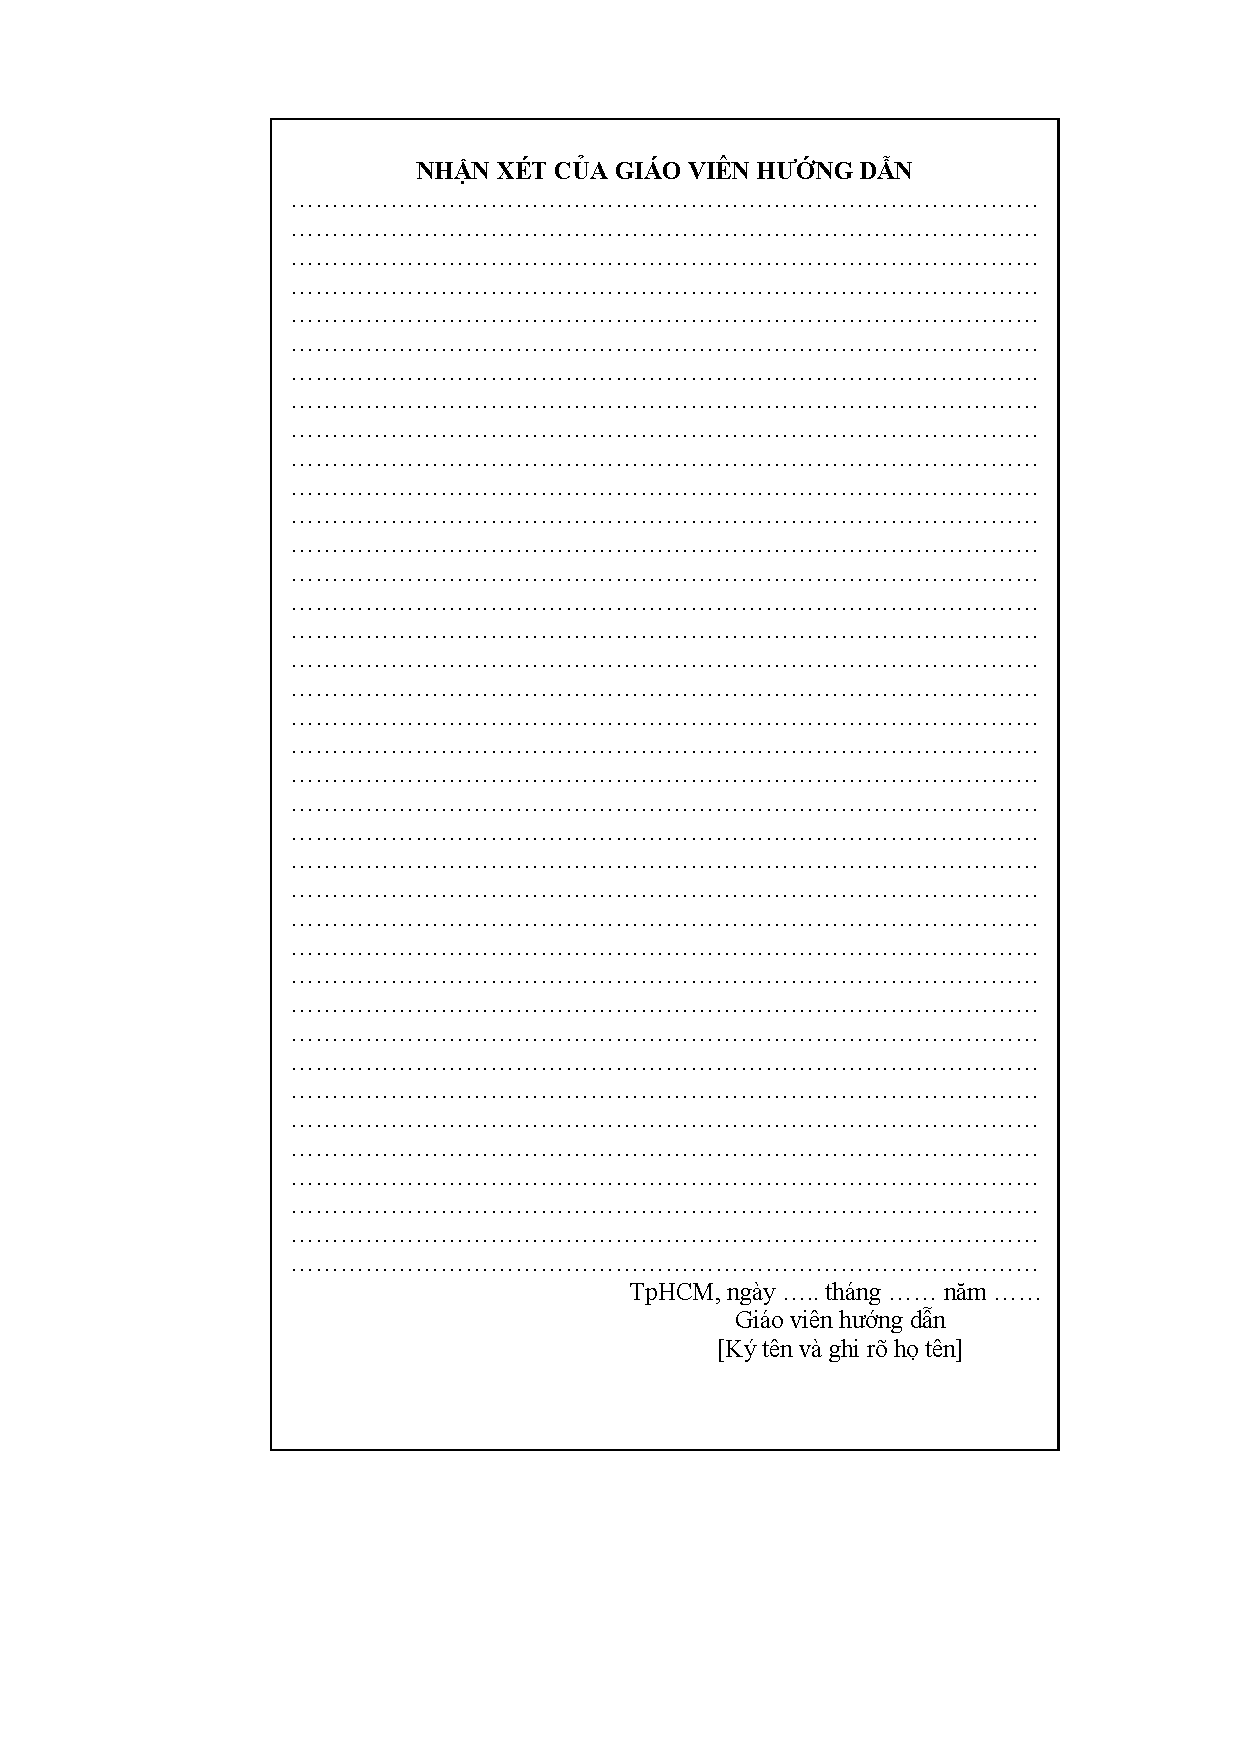
\includepdf[pages=1-2]{docs/NhanXet}
	
	\pagenumbering{roman}
	%\newpage
\chapter*{LỜI CẢM ƠN}
\addcontentsline{toc}{chapter}{LỜI CẢM ƠN}
%\hspace{0.3in}
Trước tiên, chúng em xin gửi lời tri ân sâu sắc đến Thầy Trần Trung Kiên. Thầy đã rất tận tâm, nhiệt tình hướng dẫn và chỉ bảo chúng em trong suốt quá trình thực hiện khóa luận. Không có sự quan tâm, chỉ dẫn chu đáo của Thầy chắc chắn chúng em không thể hoàn thành luận văn này.

Chúng em xin chân thành cảm ơn quý Thầy Cô khoa Công Nghệ Thông Tin - trường đại học Khoa Học Tự Nhiên, những người đã ân cần giảng dạy, xây dựng cho chúng em một nền tảng kiến thức vững chắc. 

Chúng con xin cảm ơn ba mẹ đã sinh thành, nuôi dưỡng, và dạy dỗ để chúng con có được thành quả như ngày hôm nay. Ba mẹ luôn là nguồn động viên, nguồn sức mạnh hết sức lớn lao mỗi khi chúng con gặp khó khăn trong cuộc sống.

\hfill TP. Hồ Chí Minh, 7/2016

\hfill \textit{Chiêm Duy Bảo - Vũ Đức Tài}

	
	%\newpage
	%\thispagestyle{empty}
	%\mbox{}
	
	%\newpage
	%\addcontentsline{toc}{chapter}{ĐỀ CƯƠNG CHI TIẾT}
	%\includepdf[pages=1-2,pagecommand=\thispagestyle{plain}]{docs/DeCuongChiTiet}
	
	%\include{Abstract/abstract}
	
	\newpage
	\renewcommand{\contentsname}{\centerline{MỤC LỤC}}
	\addcontentsline{toc}{chapter}{MỤC LỤC}
	\tableofcontents
	
	\newpage
	\renewcommand\listfigurename{\centerline{DANH MỤC HÌNH ẢNH}}
	\addcontentsline{toc}{chapter}{DANH MỤC HÌNH ẢNH}
	\listoffigures
	
	
	\newpage
	\renewcommand\listtablename{\centerline{DANH MỤC BẢNG}}
	\addcontentsline{toc}{chapter}{DANH MỤC BẢNG}
	\listoftables
	
	
	%\input{Abstract}
	\newpage
	\pagenumbering{arabic}
	
	\chapter{Giới thiệu}

\ifpdf
\graphicspath{{Chapter1/Chapter1Figs/PNG/}{Chapter1/Chapter1Figs/PDF/}{Chapter1/Chapter1Figs/}}
\else
\graphicspath{{Chapter1/Chapter1Figs/EPS/}{Chapter1/Chapter1Figs/}}
\fi

Những năm gần đây, \textbf{học tăng cường} (reinforcement learning) liên tục đạt được những thành tựu quan trọng trong lĩnh vực Trí tuệ nhân tạo. 
Những đóng góp nổi bật của học tăng cường bao gồm: tự động điều khiển robot di chuyển, điều khiển mô hình máy bay trực thăng, hệ thống chơi cờ vây ... 
Trong số các thành tựu này, hệ thống chơi cờ vây với khả năng chiến thắng những kỳ thủ hàng đầu thế giới là một cột mốc quan trọng của lĩnh vực Trí tuệ nhân tạo \footnote{\url{https://deepmind.com/alpha-go}}. 
Dù vậy, học tăng cường không phải là một phương pháp mới được phát triển gần đây.
Nền tảng lý thuyết của học tăng cường đã được xây dựng từ những năm 1980 \cite{sutton1998introduction}.

Được xây dựng nhằm mô phỏng quá trình học của con người, ý tưởng chính của học tăng cường là tìm cách lựa chọn hành động tối ưu để nhận được \textbf{nhiều nhất giá trị điểm thưởng} (reward). 
Giá trị điểm thưởng này có ý nghĩa tương tự cảm nhận của con người về môi trường. 
Khi một đứa trẻ bắt đầu ``học'' về thế giới xung quanh của mình, những cảm giác như đau đớn (ứng với điểm thưởng thấp) hay vui sướng (điểm thưởng cao) chính là mục tiêu cần tối ưu của việc học. 
Việc đứa trẻ thực hiện các hành động để tăng cảm giác vui sướng (và giảm đau đớn) cũng tương đồng với việc hệ thống học tăng cường tối đa hoá giá trị điểm thưởng.
Một điểm quan trọng của học tăng cường là các thuật toán được xây dựng với ít giả định nhất có thể về môi trường xung quanh.
Hệ thống sử dụng học tăng cường (agent) không cần biết cách thức hoạt động của môi trường để hoạt động. 
Ví dụ như để điều khiển robot tìm được đi trong mê cung, hệ thống không cần biết mê cung được xây dựng thế nào hay kích thước là bao nhiêu. 
Việc hạn chế tối đa những ràng buộc về dữ liệu đầu vào giúp cho thuật toán học tăng cường có thể áp dụng vào nhiều bài toán thực tế.

Học tăng cường được xem là một nhánh trong lĩnh vực máy học ngoài hai nhánh: \textit{học có giám sát} và \textit{học không có giám sát}. 
Trong bài toán học có giám sát, dữ liệu học thường được gán nhãn thủ công sẵn (hand-labeled); hệ thống cần tìm mối liên hệ giữa dữ liệu và nhãn tương ứng.
Mối liên hệ tìm được sẽ dùng để dự đoán nhãn của dữ liệu mới.
Các nhãn này có thể xem như là sự hướng dẫn trong quá trình học; tính đúng sai của việc học lúc này có thể được xác định dựa vào kết quả dự đoán của hệ thống và nhãn đúng của dữ liệu. 
Tiếp theo đối với những bài toán học không có giám sát, dữ liệu học thường không được gán nhãn nên công việc của việc học là phải tự tìm ra được cấu trúc ``ẩn'' bên dưới dữ liệu đó. 
Khác với hai loại bài toán vừa nêu, trong bài toán học tăng cường, hệ thống không nhận được nhãn thực sự (tức hành động tối ưu của tình huống hiện tại) mà chỉ nhận được điểm thưởng từ môi trường. 
Điểm thưởng lúc này chỉ thể hiện mức độ ``tốt/xấu'' của hành động vừa chọn chứ không nói lên hành động đó có phải là hành động tối ưu hay không. 
Điểm thưởng này thông thường rất \textbf{thưa}: ta có thể chỉ nhận được điểm thưởng có ý nghĩa (khác không) sau hàng trăm hành động. 
Ngoài ra, giá trị điểm thưởng thường không đơn định và rất \textbf{nhiễu}: cùng một hành động tại cùng một trạng thái, ta có thể nhận được điểm thưởng khác nhau vào hai thời điểm khác nhau. 
Hai vấn đề này (tính thưa và nhiễu của điểm thưởng) cũng chính là những khó khăn cơ bản của bài toán học tăng cường.

Game thường hay có điểm số mà người chơi cần phải tối ưu hoá. 
Đặc điểm này trùng với yêu cầu của bài toán học tăng cường, vì vậy game cũng chính là những ứng dụng tự nhiên nhất của phương pháp học tăng cường. 
Trong khoá luận này, chúng em áp dụng phương pháp học tăng cường nhằm xây dựng \textbf{hệ thống tự động chơi các game} trên hệ máy Atari. 
Dữ liệu đầu vào của hệ thống chỉ bao gồm các frame ảnh RGB cùng với điểm số. 
Từ hình ảnh thô này, hệ thống cần tìm cách chơi sao cho điểm số cuối màn chơi (episode) là lớn nhất có thể.
Lưu ý rằng điểm số này được game cung cấp cho hệ thống dưới dạng số thực (chứ không cần phải nhìn hình ảnh thô để ``đọc'' điểm số).
Điểm khó khăn của bài toán này là hệ thống hoàn toàn không biết quy luật của game trước khi bắt đầu quá trình học mà phải tự tìm hiểu quy luật và chiến thuật chơi tối ưu. 
Lý do khoá luận sử dụng game của máy Atari là vì các game này có quy luật chơi tương đối đơn giản nhưng lại rất đa dạng. 
Mỗi màn chơi thường có độ dài vừa phải (từ 2 - 15 phút) và số hành động có ý nghĩa không quá nhiều (18 hành động). 
Ngoài ra, các trò chơi này có thể được giả lập trên máy vi tính với tốc độ cao, giúp quá trình học được tăng tốc.

\begin{figure}
	\centering
	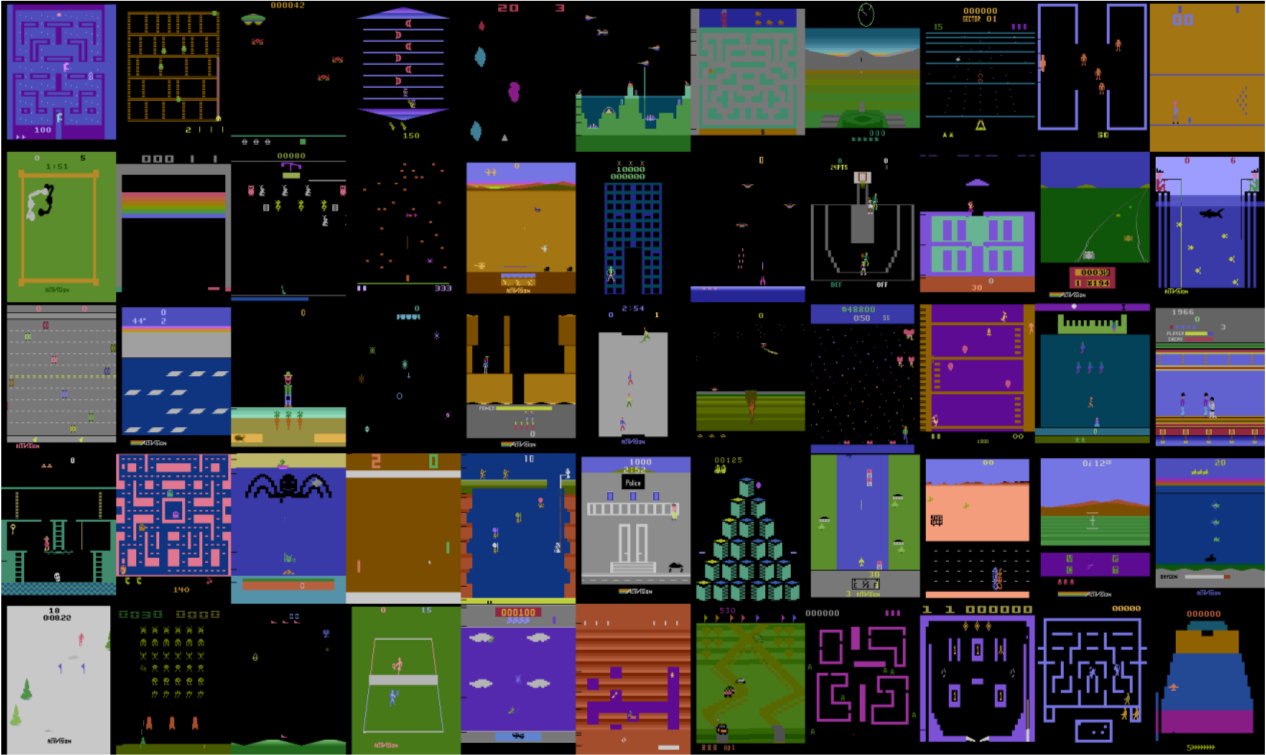
\includegraphics[width=\textwidth]{ale_55_games}
	\caption[Hình ảnh các game trên hệ máy Atari]{Hình ảnh các game trên hệ máy Atari.
	Hình được chỉnh sửa từ \cite{defazio2014comparison}}
	\label{Ale55Games}
\end{figure}

Một số khó khăn trước mắt có thể thấy ở bài toán tự động chơi game bao gồm:
\begin{itemize}
	\item \textbf{Hệ thống không biết luật chơi của game}. 
	Chính vì thế nó cũng không thể biết được hành động nào nên làm hoặc không nên làm ứng với từng tình huống cụ thể.
	\item \textbf{Dữ liệu đầu vào là hình ảnh thô} (ảnh RGB có kích thước $210\times160$). 
	Để học được một chiến thuật chơi đơn giản thì hệ thống cũng phải chơi ``thử và sai'' một số lượng lớn màn chơi (có thể lên đến 10000 frame). 
	Vì vậy, lượng dữ liệu đầu vào cần phải xử lý là rất lớn.
	\item \textbf{Các game rất khác nhau}.
	Khác biệt này là về cả hình ảnh lẫn nội dung của game.
	Để có thể học cách chơi của nhiều game khác nhau thì thuật toán học phải mang tính tổng quát cao, không sử dụng các tính chất riêng biệt của từng game.
	\item \textbf{Chiến thuật chơi game tốt thường phải tính toán dài hạn}.
	Chiến thuật chơi game tốt ở đây mang ý nghĩa đạt được ngang hoặc hơn điểm số mà con người đạt được.
	Những phương pháp tham lam, lựa chọn hành động để đạt điểm tối đa trong tương lai gần thường không đạt được nhiều điểm số.
\end{itemize}

%[TODO: Thêm hướng tiếp cận liên quan + các thực nghiệm + Reference]

%Nhiều phương pháp đã được đề xuất để giải quyết bài toán tự động chơi những game trên hệ máy Atari 2600. Hướng tiếp cận thông thường thường gồm hai giai đoạn [,]. Giai đoạn đầu rút trích đặc trưng từ những frame đầu vào. Trong giai đoạn này ngoài việc chọn ra những đặc trưng tốt cho việc học, nó cũng giúp giảm kích thước dữ liệu đầu vào cho mô hình học. Giai đoạn sau đó thực hiện xấp xỉ hàm 'đánh giá hành động' với đầu vào là những đặc trưng đã rút trích được trong giai đoạn đầu. Nhược điểm của hướng tiếp cận này là mô hình học phức tạp và khó khăn lựa trọn đặc trưng phù hợp cho nhiều game. 
Một trong những tiếp cận đầu tiên cho bài toán tự động chơi game là cuộc thi AAAI General Game Playing được đề xuất từ năm 2005 bởi đại học Stanford \cite{genesereth2005general}.
Trong cuộc thi này, các đội thi nhận được mô tả sơ bộ cho những game được sử dụng để thi.
Các mô hình chi tiết được thiết kế bên dưới các game này không được mô tả cho các đội chơi.
Dựa vào những thông tin nhận được, các đội chơi phải thiết kế một mô hình tổng quát để có thể chơi những game này; trong cuộc thi, họ sẽ chơi ngẫu nhiên một trong những game đã được mô tả \cite{genesereth2005general}.
Đội thắng cuộc trong cuộc thi này đã sử dụng mô hình ``Monte Carlo Tree Search'' (một mô hình phổ biến của học tăng cường) để tìm chiến lược chơi trong những game này.

Trong khoảng ba năm trở lại, tập những game trên hệ máy Atari 2600 trở nên phổ biến trong việc đánh giá khả năng của những phương pháp tiếp cận cho bài toán tự động chơi game.
Những game này bao gồm nhiều thể loại khác nhau như: đối kháng, chiến thuật...
Sự đa dạng trong cách chơi của những game Atari 2600 cùng giao diện lập trình đơn giản làm cho chúng gây được sự chú ý lớn trong cộng đồng Trí tuệ nhân tạo.
Nhiều phương pháp đã được đề xuất liên quan tới bài toán tự động chơi game trên hệ máy Atari 2600. 
Các công trình nghiên cứu như \cite{bellemare2013bayesian, icml2014c2_bellemare14, bellemare2012arcade} chia quá trình học ra thành hai bước.
Bước đầu tiên là hình ảnh game được rút trích đặc trưng bằng các phương pháp rút trích đặc trưng được thiết kế riêng biệt cho bài toán này.
Những phương pháp rút trích đặc trưng này do các nhà nghiên cứu bỏ sức tìm tòi những đặc điểm quan trọng trong bài toán tự động chơi game; các đặc điểm này sau đó sẽ giúp định hướng quá trình thiết kế phương pháp rút trích đặc trưng để lấy được những đặc trưng hữu ích.
Ví dụ như với đặc trưng ``BASS'' \cite{bellemare2012arcade}, đầu tiên hình ảnh game được thực hiện một phép loại bỏ nền (background subtraction).
Hình \ref{fig_bass_feature} mô tả kết quả của phép loại bỏ nền này.
\begin{figure}
	\centering
	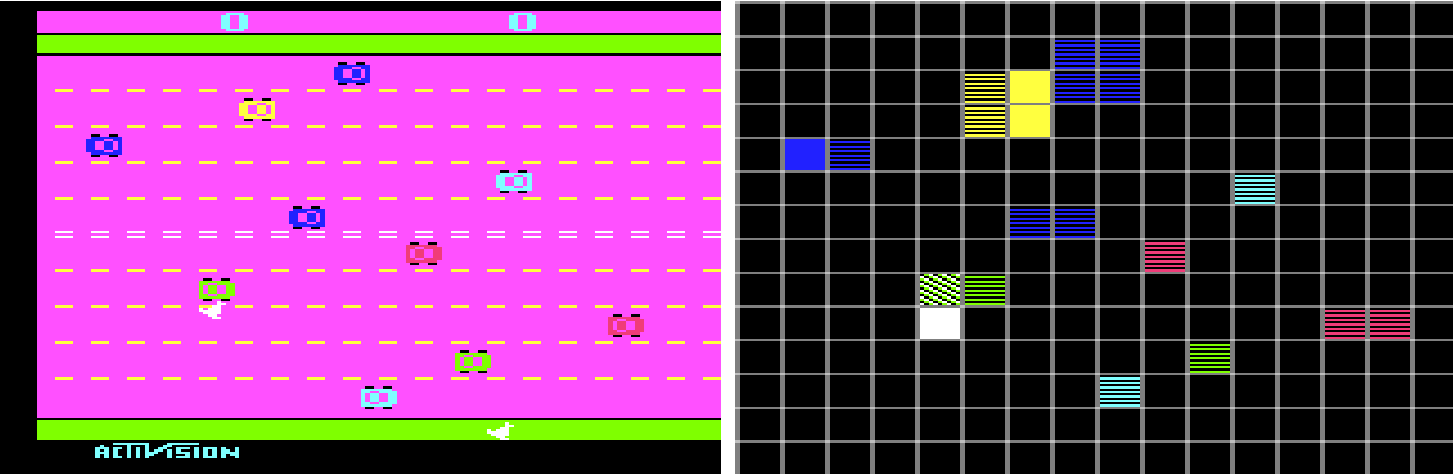
\includegraphics[width=\textwidth]{bass_feature}
	\caption[Phép loại bỏ nền của đặc trưng BASS]{Hình được chỉnh sửa từ \cite{bellemare2012arcade}.
	Hình bên trái là một hình ảnh game gốc trước khi thực hiện loại bỏ nền.
	Hình bên phải là hình ảnh sau khi thực hiện phép loại bỏ nền của đặc trưng ``BASS''.
	}
	\label{fig_bass_feature}
\end{figure}
Bước này giúp việc tìm ra các đối tượng trong hình dễ dàng hơn dựa vào nhận xét là các game Atari thường có hình nền là một màu duy nhất và các đối tượng thường có màu khác.
Tuy nhiên, đặc điểm này chỉ đúng cho các game trên hệ máy Atari nên đặc trưng ``BASS'' rất khó áp dụng cho các game khác.
Đây cũng là điểm yếu chính của các hướng tiếp cận trước đây: việc thiết kế đặc trưng bằng tay rất tốn công sức mà lại không mang tính tổng quát cao.
Bước thứ hai là các đặc trưng này được đưa vào một mô hình học như \textit{``Bayesian learning''} \cite{bellemare2013bayesian} hay \textit{hồi quy tuyến tính} \cite{bellemare2012arcade} để học chiến thuật chơi game.
Tuỳ vào độ phức tạp của đặc trưng đã được rút trích mà người ta chọn thuật toán học tương ứng.
Nếu như đặc trưng học được có kích thước quá lớn thì ta không thể áp dụng các thuật toán học phức tạp hơn được.
Tuy nhiên, thực tế cho thấy, hướng tiếp cận chia quá trình học thành hai bước như thế này tuy phức tạp nhưng lại không cho kết quả tốt \cite{mnih2013playing}.

Vào năm 2015, bài báo \textit{``Human-level control through deep reinforcement learning''} \cite{mnihdqn2015} được công bố trên tạp chí \textit{Nature}.
Bài báo này là của nhóm tác giả Volodymyr Mnih và các cộng sự thuộc nhóm nghiên cứu \textit{Google Deepmind}.
Bài báo này được coi là mở đầu cho những thành công liên tiếp rất lớn trong lĩnh vực Trí tuệ nhân tạo nói chung cũng như trong bài toán tự động chơi game nói riêng.
Sử dụng hướng tiếp cận \textbf{kết hợp học tăng cường với học sâu} (Deep learning), kết quả của bài toán tự động chơi game được cải tiến đáng kể so với những phương pháp cũ (có những game điểm số tăng hơn 20 lần \cite{mnihdqn2015}).
Thay vì chia mô hình học ra thành nhiều phần, hướng tiếp cận này xây dựng một mô hình ``end-to-end'': việc tìm chiến thuật chơi và cách rút trích đặc trưng được học cùng lúc với nhau.
Hướng tiếp cận này giúp đơn giản hoá các vấn đề gặp phải trong những hướng tiếp cận cũ và cải thiện kết quả bài toán.
Cụ thể hơn, nhờ việc áp dụng học sâu, các đặc trưng cần thiết đều được tự động học mà không cần con người tốn sức thiết kế bằng tay.
Ngoài ra, việc xây dựng một mô hình ``end-to-end'' giúp cho quá trình rút trích đặc trưng được gắn liền với việc xây dựng chiến thuật chơi; điều này giúp cho mô hình có khả năng học được những đặc trưng hữu ích cho chiến thuật chơi đó - điều mà các kỹ thuật cũ không thể thực hiện được vì các cách thiết kế đặc trưng đã được cố định trước.
Trong khoá luận này, chúng em thực hiện cài đặt lại mô hình được đề xuất bởi \cite{mnihdqn2015}.
Cùng với đó, chúng em cũng cài đặt thêm một mô hình cải tiến của \cite{mnihdqn2015} được đề xuất trong bài báo \cite{van2015deep}.
Mô hình cải tiến này giải quyết một vấn đề cụ thể của mô hình gốc và giúp cải thiện đáng kể kết quả của bài toán tự động chơi game.
Ngoài ra, về mặt cài đặt, chúng em thực hiện cài đặt tính toán song song trên GPU (Graphics Processing Unit) để tăng tốc huấn luyện.

\medskip
Phần còn lại của khoá luận được trình bày như sau:
\begin{itemize}
	\item Chương 2 trình bày kiến thức nền tảng về phương pháp học tăng cường.
	\item Chương 3 trình bày về hướng tiếp cận mà khoá luận tìm hiểu: \textbf{kết hợp học tăng cường với học sâu}.
	Đây là phần chính của khoá luận.
	\item Chương 4 trình bày kết quả thực nghiệm của hướng tiếp cận này cho bài toán tự động chơi game.
	\item Cuối cùng, kết luận và hướng phát triển được trình bày ở chương 5.
\end{itemize}
	\chapter{Kiến thức nền tảng}
\ifpdf
\graphicspath{{Chapter2/Chapter2Figs/PNG/}{Chapter2/Chapter2Figs/PDF/}{Chapter2/Chapter2Figs/}}
\else
\graphicspath{{Chapter2/Chapter2Figs/EPS/}{Chapter2/Chapter2Figs/}}
\fi
\begin{quote}
	\textit{Trong chương này sẽ trình bày những kiến thức nền tảng của học tăng cường. Trong phần đầu tiên chúng em sẽ trình bày định nghĩa của các thành phần cơ bản trong học tăng cường. Tiếp đó sẽ đề cập đến mô hình Markov Decision Processes được áp dụng trong việc đánh giá lý thuyết một số thành phần của bài toán học tăng cường. Cùng với đó sẽ trình bày qui trình tổng quát để đánh giá và cải thiện chính sách trong bài toán. Cuối cùng chúng em sẽ trình bày một số phương pháp phổ biến thường đượcAgent áp dụng để đánh giá cũng như cải thiện giúp hệ thông có cách giải tốt hơn cho bài toán trên.}
\end{quote}

\section{Các thành phần cơ bản của học tăng cường}
\subsection{Agent và môi trường}
Trong học tăng cường, đối tượng học và đưa ra quyết định được gọi chung là \textit{hệ thống}. Nó tương tác trực tiếp tới một đối tượng được gọi là \textit{môi trường}. Sự tương tác này được diễn ra liên tục. Agent lựa chọn hành động dựa trên những gì nó nhận được từ môi trường. Những thông tin này bao gồm:
\begin{itemize}
	\item \textbf{Trạng thái} (state): Những thông tin hữu ích mà hệ thống có thể cảm nhận được từ môi trường. Ví dụ trong đánh cờ, trạng thái có thể là vị trí những quân cờ đang có trên bàn cờ. Thường được ký hiệu là $s$.
	\item \textbf{Điểm thưởng} (reward): Giá trị mà môi trường trả ra tương ứng với trạng thái mà nó vừa đạt được hoặc hành động mà hệ thống vừa thực hiện. Thường được ký hiệu là $r$. Cũng với ví dụ đánh cờ, điểm thưởng mà hệ thống có thể nhận được từ môi trường trong ví dụ này là: +1 nếu hệ thống thắng, -1 nếu hệ thống thua, và trong quá trình đánh cờ điểm thưởng có thể là 0 cho mỗi trạng thái bàn cờ.
\end{itemize}
Từ trạng thái và điểm thưởng nhận được, hệ thống dựa vào đó để ra quyết định chọn hành động phù hợp sao cho cố gắng đạt được nhiều điểm thưởng nhất.

Agent và môi trường tương tác theo một chuỗi tuần tự các time-steps, $t = 0,1,2,...$. Tại mỗi time step $t$, agent nhận những mô tả trạng thái của môi trường, $\mathit{S_t} \in \mathcal{S}$, với $\mathcal{S}$ là tập các trạng thái có thể có. Dựa vào những mô tả trạng thái nhận được, agent chọn một hành động, $\mathit{A_t} \in \mathcal(\mathit{S_t})$, trong đó $\mathcal(\mathit{S_t})$ là tập các hành động có thể thực hiện tại trạng thái $\mathit{S_t}$. Tại time step sau đó, agent nhận được giá trị điểm thưởng, $\mathit{R_{t+1}} \in \mathbb{R}$, cùng với trạng thái tiếp theo $\mathit{S_{t+1}}$ Quá trình tương tác giữa agent và môi trường được mô tả trong hình \ref{AgentEnvironment}

\begin{figure}
	\centering
	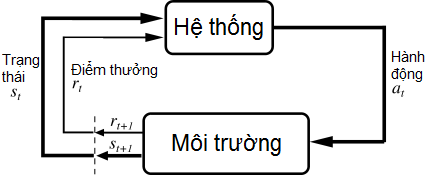
\includegraphics[width=\textwidth]{AgentEnvironment}
	\caption{Quá trình tương tác giữa hệ thông và môi trường}
	\label{AgentEnvironment}
\end{figure}

Các thành phần của agent gồm có:
\begin{itemize}
	\item \textbf{Chính sách}. Chính sách, $\pi$, xác định khả năng chọn một hành động khi hệ thống nhận được một trạng thái $s$. Chính xác tại time step $t$ được xác định $\pi_t(a \mid s) = \mathbb{P}[\mathit{A_t} = a \mid \mathit{S_t} = s]$. Để đạt được mục tiêu được nhiều điểm thưởng nhất, hệ thống cần có một chính sách chọn lựa hành động phù hợp mỗi khi gặp một trạng thái. Những phương pháp học tăng cường thường tập trung thay đổi các chính sách của hệ thống sao cho đạt được kết quả tốt trong thực nghiệm.
	\item \textbf{Hàm giá trị}. Hầu hết các thuật toán học tăng cường đầu tập trung đánh giá những hàm giá trị, các hàm này đánh giá một trạng thái hoặc hành động là tốt như thế nào cho agent thông qua việc ước lượng điểm thưởng mà hệ thống có thể nhận được ở tương lai. Thông thường, giá trị của một trạng thái $s$, dưới một chính sách $\pi$  được ký hiệu $v_{\pi}(s)$ là lượng điểm thưởng kỳ vọng nhận được bắt đầu từ trạng thái $s$ về sau.
	\item \textbf{Mô hình}. Trong một số bài toán học tăng cường, hệ thống có thể xây dựng mô hình cho riêng mình để mô phỏng lại môi trường. Qua đó cho phép hệ thống có thể suy luận hoặc dự đoán những thông tin mà nó có thể nhận được từ môi trường trong tương lai.
\end{itemize}	

\subsection{Returns}
Return $\mathit{G_t}$ xác định lượng điểm thưởng mà agent nhận được kể từ thời điểm time step $t$ đến tương lai. Return thường được xác định bằng nhiều hàm khác nhau, trong đó hàm đơn giản nhất xác định return bằng tổng các điểm thưởng có thể nhận được. Nó có dạng như sau:
\begin{equation}
\mathit{G_t} = \mathit{R_{t+1}} + \mathit{R_{t+2}} + ... + \mathit{R_{T}}
\end{equation}	
ở đây $T$ là time step cuối cùng.

Mặt khác, return cũng có thể được xác định bằng tổng điểm thưởng đã bị discount qua từng time step. Nó được định nghĩa như sau:
\begin{equation}
\mathit{G_t} = \mathit{R_{t+1}} + \gamma\mathit{R_{t+2}} + \gamma^{2}\mathit{R_{t+3}}... + \gamma^{T-1}\mathit{R_{T}} = \sum_{k=0}^{\infty}\gamma^{k}\mathit{R_{t+k+1}}
\end{equation}
Trong đó $\gamma$ là một hệ số với giá trị $0\leqslant \gamma \leqslant 1$. $\gamma$ cũng được gọi là tỉ lệ discount. Tỉ lệ này xác định độ tin tưởng của agent vào giá trị điểm thưởng ở tương lai. Khi $\gamma \to 1$, agent có su hướng quan tâm đến giá trị điểm thưởng tương lai càng nhiều. Đặc biệt với $\gamma = 0$, khi đó agent chỉ quan tâm giá trị điểm thưởng ở hiện tại mà bỏ qua những giá trị điểm thưởng ở tương lai.	

\section{Mô hình Markov Decision Processes}
%	\begin{itemize}
%			\item Các thành phần MDP
%			\item Ví dụ cho mô hình MDP
%			\item Phương trình Bellman
%			\item Qui trình đánh giá chính sách: Kỹ thuật qui hoạch động
%			\item Qui trình cải thiện chính động: Kỹ thuật qui hoạch động
%	\end{itemize}
\subsection{Định nghĩa mô hình Markov Decision Processes}
Mô hình Markov Decision Processes (MDP) được sử dụng để mô hình hóa bài toán học tăng cường một cách có hình thức. Cụ thể, MDP là một bộ bao gồm 5 thành phần $<\mathcal{S, A, P, R, \gamma}>$ trong đó:
\begin{itemize}
	\item $\mathcal{S}$: tập trạng thái hữu hạn có thể có của môi trường.
	\item $\mathcal{A}$: tập những hành động hữu hạn mà hệ thống có thể thực hiện để tương tác với môi trường.
	\item $\gamma$: Hệ số có giá trị thỏa $0\leqslant \gamma \leqslant 1$ thể hiện mức độ tin tưởng về giá trị điểm thưởng nhận được ở tương lai.
	\item $\mathcal{P}$: ma trận xác suất chuyển trạng thái. Trong đó $\mathcal{P}_{ss'}^{a}$ là xác suất chuyển đến trạng thái $s'$ khi hệ thống đang ở trạng thái $s$ và thực hiện hành động $a$.
	\begin{equation}
	\mathcal{P}_{ss'}^{a} = \mathbb{P}[\mathit{S_{t+1}} = s' \mid \mathit{S_{t}} = s, \mathit{A_{t}} = a]
	\end{equation}
	\item $\mathcal{R}$: ma trận điểm thưởng theo từng bộ (trạng thái, hành động). $\mathcal{R}_{s}^a$ là kỳ vọng giá trị điểm thưởng nhận được khi hệ thống thực hiện hành động $a$ ở trạng thái $s$.
	\begin{equation}
	\mathcal{R}_{s}^a = \mathbb{E}[\mathit{R_{t}} \mid \mathit{S_{t}} = s, \mathit{A_{t}} = a]
	\end{equation}				
\end{itemize}

\textbf{Ví dụ: Mô hình MDP trong robot thu gom} Công việc của robot này là thu lượm những lon soda đã được uống hết trong văn phòng. Nó có những cảm biến để xác định những lon soda này, bánh xe và cánh tay để di chuyển và gắp nhặt những lon này bỏ vào thùng. Robot hoạt động bằng pin sạc. Hệ thống điều khiển của robot có chức năng tiếp nhận những thông tin từ cảm biến từ đó điểu khiển bánh xe và cánh tay. Trong ví dụ, chúng em chỉ xét dựa trên mức độ pin hiện tại robot nên quyết định tìm kiếm những lon soda như thế nào? Robot có thể có ba quyết định (1) thực hiện tìm kiếm một lon soda, (2) đứng yên và đợi người khác mang lon soda đến cho nó, (3) quay trở lại nơi sạc pin. Trạng thái của môi trường được xác định là trạng thái của pin hiện tại của robot. Cách tốt nhất để tìm kiếm những lon soda là robot thực hiện hành động tìm kiếm, nhưng việc này sẽ làm giảm dung lượng của pin. Ngược lại nếu robot đứng yên và đợi thì dung lượng pin của nó không giảm. Mỗi khi dung lượng pin của robot ở mức thấp nó sẽ quay lại chỗ sạc pin. Trường hợp xấu nhất có thể xảy ra là robot không đủ dung lượng pin để quay lại nơi sạc khi đó nó sẽ đứng yên và đợi ai đó mang nó đến chỗ sạc. Do đó robot cần có một chiến lược phù hợp để đạt được hiệu năng cao nhất có thể.
Hệ thống đưa ra những quyết định của nó dựa trên mức năng lượng pin. Mức năng lượng này có thể được xác định hai mức \textit{cao} và \textit{thấp}. Khi đó tập trạng thái mà hệ thống có thể nhận được $\mathcal{S} = \left \{\text{cao}, \text{thấp} \right \}$. Những hành động của hệ thống trong ví dụ này được xét đơn giản gồm ba hành động \textit{đợi}, \textit{tìm kiếm}, và \textit{sạc pin}. Khi dung lượng pin ở trạng thái cao, hệ thống chỉ thực hiện hai hành động: tìm kiếm và đợi. Ngược lại khi ở trạng thái thấp, hệ thống có thể thực hiện ba hành động: tìm kiếm, đợi, và sạc pin.
$$\mathcal{A}(\text{cao}) =  \left \{\text{tìm kiếm}, \text{đợi} \right \}$$
$$\mathcal{A}(\text{thấp}) =  \left \{\text{tìm kiếm}, \text{đợi}, \text{sạc pin} \right \}$$

Khi mức năng lượng pin ở mức cao, việc robot thực hiện tìm kiếm sẽ có xác suất $\alpha$ năng lượng pin vẫn ở mức cao, và $1 - \alpha$ năng lượng của pi sẽ chuyển về mức thấp. Mặt khác, khi mức năng lượng ở mức thấp, nếu robot thực hiện tìm kiếm sẽ có xác suất $\beta$ năng lượng pin ở mức thấp và $1 - \beta$ chuyển đến mức cao, trường hợp này xảy ra khi dung lượng pin cạn kiệt và cần ai đó mang nó đến chỗ sạc cho đến khi đạt mức năng lượng cao. Ngoài ra, mỗi lần robot thu gom được một lon soda nó sẽ nhận được $+1$ điểm thưởng và sẽ bị $-3$ điểm thưởng mỗi khi nó phải cần ai đó mang đến chỗ sạc. $r_{\text{đợi}}$, $r_{\text{tìm kiếm}}$ là số lượng lon soda kỳ vọng mà robot có thể thu gom được trong khi đợi và tìm kiếm. Hình \ref{graphRobot} minh họa cho mô hình MDP trong robot thu gom.

%% Hình vẽ
\begin{figure}
	\centering
	\begin{tikzpicture}[node distance=6.5cm,>=stealth',bend angle=45 ,auto]
	
	\tikzstyle{state}=[circle,thick,draw=blue!75,fill=blue!20,minimum size = 15mm]
	\tikzstyle{action}=[circle,draw=black!75,
	fill=black!75,minimum size=2mm]
	
	\tikzstyle{every label}=[red]
	
	\begin{scope}
	% First net
	\node [state] (high)                           {Cao};	
	\node [state] (low) [right of=high]              {Thấp};
	
	\node [action] (w1) [above = 1.5cm of high, label=left:Đợi] {}
	edge      					(high)
	edge [post,bend right] node[left]{$1, r_{\text{đợi}}$}      (high);
	
	\node [action] (s1) [below = 1.5cm of high, label=right:Tìm kiếm] {}
	edge        				(high)
	edge [post,bend left] node[left]{$\alpha, r_{\text{tìm kiếm}}$}       (high)
	edge [post,bend right] node[below=0.2]{$1 - \alpha, r_{\text{tìm kiếm}}$}       (low);
	
	\node [action] (s2) [above = 1.5cm of low, label=left:Tìm kiếm] {}
	edge        				(low)
	edge [post,bend left] node[right]{$\beta, r_{\text{tìm kiếm}}$}       (low)
	edge [post,bend right] node[above=0.2]{$1 - \beta, -3$}       (high);
	
	\node [action] (w2) [below = 1.5cm of low, label=right:Đợi] {}
	edge        				(low)
	edge [post,bend right] node[right]{$1, r_{\text{đợi}}$}       (low);
	
	\node [action] (re) [left = 1.5cm of low, , label=above:Sạc pin] {}
	edge						(low)
	edge [post] node[above]{$1, 0$} (high);
	\end{scope}		
	\end{tikzpicture}
	\caption[Đồ thị minh họa chuyển trạng thái cho robot thu gom]{Đồ thị minh họa chuyển trạng thái cho robot thu gom. Trong đồ thị có hai loại node: node trạng thái và node hành động. Node trạng thái minh họa những trạng thái có thể có mà hệ thống có thể nhận được, nó được ký hiệu một vòng tròn lớn với tên của trạng thái bên trong. Node hành động tường ứng với cặp (trạng thái, hành động). Việc thực hiện hành động $a$ tại trạng thái $s$ tương ứng trên đồ thị là một cạnh bắt đầu từ node trạng $s$ tới node hành động $a$. Khi đó môi trường sẽ trả ra trạng thái tiếp theo $s'$ ứng với đích của mũi tên đi từ node hành động $a$. Xác suất chuyển tới trạng thái $s'$ khi thực hiện hành động $a$ ở trạng thái $s$ $p(s' \mid s,a)$, và giá trị điểm thưởng kỳ vọng nhận được trong trường hợp này $r(s,a,s')$ tương ứng với ký hiệu trên mũi tên. Ví dụ: khi mức năng lượng pin đăng ở trạng thái \textit{thấp}, hệ thống quyết định thực hiện hành động \textit{sạc pin} khi đó trạng thái tiếp theo mà hệ thống nhận được sẽ là mức năng lượng pin ở trạng thái \textit{cao} và xác suất chuyển tới trạng thái \textit{cao} $p(\text{cao} \mid \text{thấp}, \text{sạc pin})$ là 1 và giá trị kỳ vọng điểm thưởng tương ứng $r(\text{thấp}, \text{sạc pin}, \text{cao})$ là 0.}
	\label{graphRobot}
\end{figure}

%% ----------------------------------------------------

\subsection{Chính sách và hàm giá trị} \label{sec:policy_value}
Một chính sách $\pi$ xác định xác suất mà hệ thông thực hiện hành động $a$ khi nó trong trạng thái $s$ được ký hiệu $\pi(a \mid s)$. Có thể nói chính sách như "bộ não" của hệ thống, nó quyết định cách thức mà hệ thống hành động trong những trạng thái cụ thể do đó một chính sách tốt cũng làm cho khả năng hệ thống ra quyết định trở nên tốt hơn.

Hàm giá trị cho biết những trạng thái hoặc những cặp hành động và trạng thái tốt như thế nào cho hệ thông khi nó trong những trạng thái hoặc thực hiện những cặp hành động và trạng thái đó. Khái niệm tốt ở đây nghĩa là giá trị điểm thưởng kỳ vọng mà hệ thông có thể nhận được ở tương lai. Hầu hết các thuật toán trong học tăng cường đều tập trung vào việc đánh giá những hàm giá trị qua đó cải thiện chính sách trở nên tốt hơn. Điểm thưởng mà hệ thống có thể nhận được trong tương lai phụ thuộc vào những hành động mà nó thực hiện. Do đó hàm giá trị chịu ảnh hưởng rất nhiều vào chính sách. Giá trị của trạng thái $s$ dưới một chính sách $\pi$, ký hiệu $v_{\pi}(s)$, là giá trị kỳ vọng của return mà hệ thống nhận được bắt đầu từ trạng thái $s$ theo chính sách $\pi$ sau đó. Với mô hình MDP, $v_{\pi}(s)$ được định nghĩa như sau:
\begin{equation}
v_{\pi}(s) = \mathbb{E}_{\pi}\left [\mathit{G}_t \mid \mathit{S}_{t} = s\right ] = \mathbb{E}_{\pi}\left [\sum_{k = 0}^{\infty}\gamma^{k}\mathit{R}_{t+k+1} \middle|\ \mathit{S}_t= s\right ]
\end{equation}
$v_{\pi}$ được gọi là hàm giá trị trạng thái dưới chính sách $\pi$.

Tương tự, chúng ta định nghĩa giá trị của việc thực hiện hành động $a$ trong trạng thái $s$ dưới chính sách $\pi$, được ký hiệu $q_{\pi}(s,a)$, là giá trị kỳ vọng của return mà hệ thống nhận được bắt đầu từ việc thực hiện hành động $a$ trong trạng thái $s$ theo chính sách $\pi$
\begin{equation}
\label{action_value}
q_{\pi}(s,a) = \mathbb{E}_{\pi}\left [\mathit{G}_t \mid \mathit{S}_{t} = s, \mathit{A}_{t} = a  \right ] = \mathbb{E}_{\pi}\left [\sum_{k = 0}^{\infty}\gamma^{k}\mathit{R}_{t+k+1} \middle|\ \mathit{S}_t= s, \mathit{A}_{t} = a \right ]
\end{equation}
$q_{\pi}$ được gọi là hàm giá trị hành động dưới chính sách $\pi$.

Hình \ref{fig:relationship_value_functions} minh họa quan hệ giữa hàm giá trị trạng thái và hàm giá trị hành động, khi có được hàm giá trị này ta có thể có được hàm giá trị còn lại. Phương trình \ref{eq:relation_value_action} xác hàm giá trị của một trạng thái bằng giá trị kỳ vọng giá trị của các hành động thực hiện tại trạng thái đó. Hình \ref{fig:relationship_value_functions}a minh họa quan hệ giữa giá trị của một trạng thái $s$ và giá trị của các hành động thực hiện tại trạng thái đó. Hình \ref{fig:relationship_value_functions}b cho thấy từ việc thực hiện hành động $a$ tại trạng thái $s$, môi trường có thể trả ra nhiều trạng thái tiếp theo $s'$ khác nhau. Do đó giá trị của hành động $a$ ở trạng thái $s$ có thể được xác định bằng tổng giá trị kỳ vọng điểm thưởng nhận được và giá trị kỳ vọng của các trạng thái tiếp theo đó đã được nhân với hệ số $\gamma$. Cách xác định này được biểu diễn trong phương trình \ref{eq:relation_action_value}.
\begin{align}
v_{\pi} = {} & \sum_{a \in \mathcal{A}(s)}^{}\pi(a \mid s)q_{\pi}(s,a) \label{eq:relation_value_action}\\
q_{\pi}(s,a) = {} & \mathcal{R}_{s}^{a} + \gamma \sum_{s' \in \mathcal{S}}^{}\mathcal{P}_{ss'}^{a}v_{\pi}(s') \label{eq:relation_action_value}
\end{align}
%----------------------------------------	
\begin{figure}
	\centering
	\begin{tikzpicture}[node distance=4.5cm,>=stealth',bend angle=45,auto]
	
	\tikzstyle{state}=[circle,thick,draw=blue!75,fill=white!20,minimum size = 5mm, inner sep=0pt]
	\tikzstyle{action}=[circle,draw=black!75,
	fill=black!75,minimum size=2mm]
	
	\tikzstyle{every label}=[red]
	
	\begin{scope}
	% First net
	\node [state, label={[name=label node]right:$s \mapsto v_{\pi}(s)$}] (s1)      {};
	
	\node (label) [left = 2cm of s1] {(a)};
	
	\node [action, label={[name=label node]right:$a \mapsto q_{\pi}(s,a)$}] (a1) [below right = 2 cm and 1 cm of s1]    {}
	edge node[right]{$r$} (s1);	
	
	\node [action] (a2) [below left  = 2 cm and 1 cm of s1]    {}
	edge (s1);
	
	\end{scope}		
	
	\begin{scope}[xshift=8cm]
	% Second net		
	\node [action, label={[name=label node]right:$s,a \mapsto q_{\pi}(s,a)$}] (a4)      {};		
	\node (label) [left = 2cm of a4] {(b)};		
	\node [state] (s8) [below right = 2 cm and 1 cm of a4, label=right:$s' \mapsto v_{\pi}(s')$]    {}
	edge node[right]{$r$} (a4);		
	\node [state] (s9) [below left  = 2 cm and 1 cm of a4]    {}
	edge (a4);		
	\end{scope}		
	\end{tikzpicture}		
	\caption[Đồ thị minh họa quan hệ giữa những hàm giá trị]{Đồ thị minh họa quan hệ giữa hàm giá trị trạng thái và hàm giá trị hành động}
	\label{fig:relationship_value_functions}
\end{figure}

%----------------------------------------
\begin{figure}
	\centering
	\begin{tikzpicture}[node distance=4.5cm,>=stealth',bend angle=45,auto]
	
	\tikzstyle{state}=[circle,thick,draw=blue!75,fill=white!20,minimum size = 5mm, inner sep=0pt]
	\tikzstyle{action}=[circle,draw=black!75,
	fill=black!75,minimum size=2mm]
	
	\tikzstyle{every label}=[red]
	
	\begin{scope}
	% First net
	\label{fig_bellman_value}
	\node [state, label=above:$s$] (s1)                           {};
	
	\node (label) [left = 2cm of s1] {(a)};
	
	\node [action] (a1) [below = 2cm of s1]              {}
	edge (s1);
	
	\node [action] (a2) [left = 2cm of a1]              {}
	edge (s1);
	
	\node [action] (a3) [right = 2cm of a1, label=right:$a$]              {}
	edge (s1);
	
	\node [state] (s2) [below left = 2cm and 0.3cm of a1] {}
	edge (a1);
	
	\node [state] (s3) [below right = 2cm and 0.3cm of a1] {}
	edge (a1);
	
	\node [state] (s4) [below left = 2cm and 0.3cm of a2] {}
	edge (a2);
	
	\node [state] (s5) [below right = 2cm and 0.3cm of a2] {}
	edge (a2);
	
	\node [state] (s6) [below left = 2cm and 0.3cm of a3] {}
	edge (a3);
	
	\node [state] (s7) [below right = 2cm and 0.3cm of a3, label=right:$s'$] {}
	edge node[right]{$r$} (a3);	
	\end{scope}
	
	\begin{scope}[xshift=8cm]
	% Second net
	\label{fig_bellman_action}
	\node [action, label={[name=label node]above:$s,a$}] (a4)      {};
	
	\node (label) [left = 2cm of a4] {(b)};
	
	\node [state] (s8) [below right = 2 cm and 1 cm of a4, label=right:$s'$]    {}
	edge node[right]{$r$} (a4);	
	
	\node [state] (s9) [below left  = 2 cm and 1 cm of a4]    {}
	edge (a4);
	
	\node [action] (a5) [below left  = 2 cm and 0.3 cm of s8]    {}
	edge (s8);
	
	\node [action] (a6) [below right  = 2 cm and 0.3 cm of s8, label=right:$a'$]    {}
	edge (s8);
	
	\node [action] (a7) [below left  = 2 cm and 0.3 cm of s9]    {}
	edge (s9);
	
	\node [action] (a8) [below right  = 2 cm and 0.3 cm of s9]    {}
	edge (s9);	
	
	\end{scope}
	
	\end{tikzpicture}
	\caption[Đồ thị minh họa cho hàm giá trị]{Đồ thị minh họa cho (a) $v_{\pi}$ và (b) $q_{\pi}$}
	\label{backup_diagram}
\end{figure}

Hàm giá trị có một tính chất cơ bản thường được áp dụng trong học tăng cường đó là mối quan hệ đệ quy. Cho bất kỳ chính sách $\pi$ với bất kỳ trạng thái $s$, hàm giá trị cho một trạng thái được xác định:	
\begin{align}
\label{bell_state}
%\begin{aligned}
v_{\pi}(s) = {}& \mathbb{E}_{\pi}\left [\mathit{G}_t \mid \mathit{S}_{t} = s\right ] \nonumber \\
= {}& \mathbb{E}_{\pi}\left [ \mathit{R}_{t+1} + \gamma \mathit{R}_{t+2} + \gamma^{2} \mathit{R}_{t+3} + ... \mid \mathit{S}_t = s  \right ] \nonumber \\
= {}& \mathbb{E}_{\pi}\left [ \mathit{R}_{t+1} + \gamma( {R}_{t+2} + \gamma \mathit{R}_{t+3} + ...) \mid \mathit{S}_t = s  \right ] \nonumber \\
= {}& \mathbb{E}_{\pi}\left [ \mathit{R}_{t+1} + \gamma\mathit{G}_{t + 1} \mid \mathit{S}_t = s  \right ] \nonumber \\
= {}& \mathbb{E}_{\pi}\left [ \mathit{R}_{t+1} + \gamma v(\mathit{S}_{t+1}) \mid \mathit{S}_t = s  \right ]
%\end{aligned}
\end{align}	
Phương trình \ref{bell_state} được gọi là phương trình Bellman cho $v_{\pi}$. Từ phương trình này ta thấy được mối liên quan giữa giá trị của một trạng $s$ bất kỳ và giá trị của những trạng thái tiếp theo đạt được từ trạng thái đó. Ý tưởng nhìn trước một bước, hay nói cách khác đánh giá trạng thái hiện tại bằng cách nhìn trước tất cả những trạng tái tiếp theo có thể đạt được từ trạng thái đó, được minh họa trong hình \ref{backup_diagram}a. Từ một trạng thái, môi trường có thể trả ra nhiều điểm thưởng $r$ và trạng thái tiếp theo $s'$ khác nhau. Phương trình \ref{bell_state} sẽ trung bình tất cả các trường hợp có thể đó lại theo xác suất mà chúng xuất hiện. Phương trình này cũng cho thấy giá trị của một trạng thái phải bằng tổng giá trị kỳ vọng của những trạng thái tiếp sau đó và giá trị kỳ vọng điểm thưởng nhận được.

\begin{equation}
\label{bell_action}
q_{\pi}(s,a) = \mathbb{E}_{\pi} \left[\mathit{R}_{t+1} + \gamma q_{\pi}(\mathit{S}_{t+1}, \mathit{A}_{t+1}) \mid \mathit{S}_t = s, \mathit{A}_t = a \right]
\end{equation}

Phân tích phương trình \ref{action_value} tương tự như đã làm đối với hàm giá trị hành động, ta có được phương trình \ref{bell_action}. Hình \ref{backup_diagram}b minh họa ý tưởng nhìn trước một đước để đánh giá giá trị của một hành động ở trạng thái hiện tại. Từ một hành động $a$ ở trạng thái $s$, môi trường có thể trả ra nhiều điểm thưởng $r$ và trạng thái $s'$ khác nhau. Trong mỗi trạng thái $s'$ lại có nhiều hành động $a'$ khác nhau có thể thực hiện.	Phương trình \ref{bell_action} sẽ trung bình tất cả các trường hợp có thể đó lại theo xác suất mà chúng được thực hiện. Hay nói cách khác, phương trình \ref{bell_action} cho thấy giá trị của một hành động $a$ tại trạng thái $s$, $q_{\pi}(a,s)$ cũng được xác định tổng bằng giá trị kỳ vọng điểm thưởng hệ thống nhận được nhận được ngay sau khi thực hiện thực hiện hành động đó và giá trị kỳ vọng của các hành động trong những trạng thái kế tiếp.

\subsection{Hàm giá trị tối ưu}
Để giải quyết những vấn đề trong học tăng cường, chúng ta cần tìm một chính sách sao cho hệ thống có thể đạt được nhiều điểm thưởng nhất có thể. Một chính sách $\pi$ được xác định là tốt hơn hoặc bằng chính sách $\pi'$ khi giá trị kỳ vọng của return theo chính sách $\pi$ lớn hơn hoặc bằng giá trị đó theo chính sách $\pi'$. Hay có thể định nghĩa theo cách khác:
\begin{equation}
\pi \geq \pi' \Longleftrightarrow v_{\pi}(s) \geq v_{\pi'}(s), \forall s \in \mathcal{S}
\end{equation}

Luôn có ít nhất một chính sách tốt hơn hoặc bằng tất cả các chính sách còn lại \cite{sutton1998introduction}. Chúng được gọi chung là \textit{chính sách tối ưu} và được ký hiệu $\pi_{*}$. Những chính sách tối ưu đều cùng có chung một hàm giá trị trạng thái và hàm giá trị hành động. Hai loại hàm giá trị này có thể được gọi chung là \textit{hàm giá trị tối ưu}. Chúng ta cũng có thể gọi tách biệt \textit{hàm giá trị trạng thái tối ưu} đối với hàm giá trị trạng thái và \textit{hàm giá trị hành động tối ưu} đối với hàm giá trị hành động. Phương trình \ref{eq:optimal_state} và \ref{eq:optimal_action} định nghĩa hình thức cho hai loại hàm này
\begin{align}
v_{*}(s) = {} & \max_{\pi}v_{\pi}(s), \forall s \in \mathcal{S} \label{eq:optimal_state} \\
q_{*}(s,a) = {} & \max_{\pi}q_{\pi}(s,a), \forall s \in \mathcal{S} \text{ và } \forall a \in \mathcal{A}(s) \label{eq:optimal_action}
\end{align}
Từ hai phương trình \ref{eq:optimal_state} và \ref{eq:optimal_action} thấy rằng để xác định hàm giá trị tối ưu của mỗi trạng thái $s$ hoặc cặp trạng thái và hành động ($s,a$), ta cần thử đánh giá giá trị của chúng theo tất cả các chính sách có thể có và chọn giá trị cao nhất là giá trị tối ưu cho trạng thái $s$ hoặc cặp trạng thái và hành động ($s,a$).

Hình \ref{fig:relationship_optimal_functions} minh họa quan hệ giữa giá trị trạng thái tối ưu và hàm giá trị hành động tối ưu, khi có được hàm này ta dễ dàng có được hàm còn lại. Trong hình \ref{fig:relationship_optimal_functions}a, ta có thể xác định giá trị tối ưu cho trạng thái $s$ dựa trên hàm giá trị hành động tối ưu của các hành động có thể thực hiện tại trạng thái đó. Phương trình \ref{eq:optimal_state_action} xác định giá trị tối ưu cho trạng thái $s$ bằng cách chọn giá trị hành động tối ưu lớn nhất trong các hành động có thể thực hiện ở trọng thái đó. Tương tự trong hình \ref{fig:relationship_optimal_functions}b, ta có thể xác định giá trị tối ưu cho hành động $a$ ở trạng thái $s$, dựa trên hàm giá trị trạng thái tối ưu của các trạng thái kế tiếp đạt được từ hành động đó. Phương trình \ref{eq:optimal_action_state} xác định giá trị tối ưu của hành động $a$ tại trạng thái $s$ bằng tổng giá trị kỳ vọng điểm thưởng nhận được từ môi trường và giá trị tối ưu kỳ vọng của những trạng thái kế tiếp đã nhân với hệ số $\gamma$.

\begin{figure}
	\centering
	\begin{tikzpicture}[node distance=4.5cm,>=stealth',bend angle=45,auto]
	
	\tikzstyle{state}=[circle,thick,draw=blue!75,fill=white!20,minimum size = 5mm, inner sep=0pt]
	\tikzstyle{action}=[circle,draw=black!75,
	fill=black!75,minimum size=2mm]
	
	\tikzstyle{every label}=[red]
	
	\begin{scope}
	% First net
	\node [state, label={[name=label node]right:$s \mapsto v_{*}(s)$}] (s1)      {};
	
	\node (label) [left = 2cm of s1] {(a)};
	
	\node [action, label={[name=label node]right:$a \mapsto q_{*}(s,a)$}] (a1) [below right = 2 cm and 1 cm of s1]    {}
	edge node[right]{$r$} (s1);	
	
	\node [action] (a2) [below left  = 2 cm and 1 cm of s1]    {}
	edge (s1)
	pic[draw=black, -, angle eccentricity=1.2, angle radius=1cm]
	{angle=a2--s1--a1};
	
	\end{scope}		
	
	\begin{scope}[xshift=8cm]
	% Second net		
	\node [action, label={[name=label node]right:$s,a \mapsto q_{*}(s,a)$}] (a4)      {};		
	\node (label) [left = 2cm of a4] {(b)};		
	\node [state] (s8) [below right = 2 cm and 1 cm of a4, label=right:$s' \mapsto v_{*}(s')$]    {}
	edge node[right]{$r$} (a4);		
	\node [state] (s9) [below left  = 2 cm and 1 cm of a4]    {}
	edge (a4);		
	\end{scope}		
	\end{tikzpicture}		
	\caption[Đồ thị minh họa quan hệ giữa những hàm giá trị tối ưu]{Đồ thị minh họa quan hệ giữa hàm giá trị trạng thái tối ưu và hàm giá trị hành động tối ưu}
	\label{fig:relationship_optimal_functions}
\end{figure}	
\begin{align}
%		q_{*}(s,a) = \mathbb{E} \left[ \mathit{R}_{t+1} + \gamma v_{*}(\mathit{S}_{t+1}) \mid \mathit{S}_{t} = s, \mathit{A}_{t} = a \right]
v_{*}(s) = {} & \max_{a \in \mathcal{A}(s)} q_{*}(s,a) \label{eq:optimal_state_action}\\
q_{*}(s,a) = {} & \mathit{R}_{s}^{a} + \gamma \sum_{s' \in \mathcal{S}}^{} \mathcal{P}_{ss'}^{a} v_{*}(s') \label{eq:optimal_action_state} \\
v_{*}(s) = {} & \max_{a \in \mathcal{A}(s)} \mathit{R}_{s}^{a} + \gamma \sum_{s' \in \mathcal{S}}^{} \mathcal{P}_{ss'}^{a} v_{*}(s') \label{eq:bellman_optimal_state}\\
q_{*}(s,a) = {} & \mathit{R}_{s}^{a} + \gamma \sum_{s' \in \mathcal{S}}^{} \mathcal{P}_{ss'}^{a} \max_{a' \in \mathcal{A}(s')} q_{*}(s',a') \label{eq:bellman_optimal_action}		
\end{align}

\begin{figure}
	\centering
	\begin{tikzpicture}[node distance=4.5cm,>=stealth',bend angle=45,auto]
	
	\tikzstyle{state}=[circle,thick,draw=blue!75,fill=white!20,minimum size = 5mm, inner sep=0pt]
	\tikzstyle{action}=[circle,draw=black!75,
	fill=black!75,minimum size=2mm]
	
	\tikzstyle{every label}=[red]
	
	\begin{scope}
	
	\node [state, label={[name=label node]right:$s \mapsto v_{*}(s)$}] (s1)      {};
	
	\node (label) [left = 2cm of s1] {(a)};
	
	\node [action] (a1) [below right = 2 cm and 1 cm of s1, label=right:$a$]    {}
	edge(s1);
	
	\node [action] (a2) [below left  = 2 cm and 1 cm of s1]    {}
	edge (s1)
	pic[draw=black, -, angle eccentricity=1.2, angle radius=1cm]
	{angle=a2--s1--a1};
	
	\node [state] (s2) [below left  = 2 cm and 0.3 cm of a1]    {}
	edge (a1);
	
	\node [state, label={[name=label node]right:$s' \mapsto v_{*}(s')$}] (s3) [below right  = 2 cm and 0.3 cm of a1]    {}
	edge node[right]{$r$}	 (a1);
	
	\node [state] (s4) [below left  = 2 cm and 0.3 cm of a2]    {}
	edge (a2);
	
	\node [state] (s5) [below right  = 2 cm and 0.3 cm of a2]    {}
	edge (a2);	
	\end{scope}
	
	\begin{scope}[xshift=8cm]
	
	\node [action, label={[name=label node]right:$(s,a) \mapsto q_{*}(s,a)$}] (a3)      {};
	
	\node (label) [left = 2cm of a3] {(b)};
	
	\node [state] (s6) [below right = 2 cm and 1 cm of a3, label=right:$s'$]    {}
	edge node[right]{$r$} (a3);	
	
	\node [state] (s7) [below left  = 2 cm and 1 cm of a3]    {}
	edge (a3);
	
	\node [action] (a4) [below left  = 2 cm and 0.3 cm of s6]    {}
	edge (s6);
	
	\node [action, label={[name=label node]right:$a' \mapsto q_{*}(s',a')$}] (a5) [below right  = 2 cm and 0.3 cm of s6]    {}
	edge (s6)
	pic[draw=black, -, angle eccentricity=1.2, angle radius=1cm]
	{angle=a4--s6--a5};
	
	\node [action] (a6) [below left  = 2 cm and 0.3 cm of s7]    {}
	edge (s7);
	
	\node [action] (a7) [below right  = 2 cm and 0.3 cm of s7]    {}
	edge (s7)
	pic[draw=black, -, angle eccentricity=1.2, angle radius=1cm]
	{angle=a6--s7--a7};
	
	\end{scope}		
	\end{tikzpicture}
	\caption[Đồ thị minh họa phương trình Bellman trong hàm giá trị tối ưu]{Đồ thị minh họa phương trình Bellman trong (a) $v_{*}$} và (b) $q_{*}$
	\label{fig:bellman_optimal_function}
\end{figure}

Phương trình \ref{eq:bellman_optimal_state} và \ref{eq:bellman_optimal_action} dễ dàng có được bằng cách thay thế hai phương trình \ref{eq:optimal_state_action} và \ref{eq:optimal_action_state} qua lại lẫn nhau. Từ hai phương trình này, ta thấy được dạng phương trình Bellman trong hàm giá trị trạng thái tối ưu và hàm giá trị hành động tối ưu. Hình \ref{fig:bellman_optimal_function} minh họa ý tưởng nhìn trước một bước của phương trình Bellman trong hàm giá trị tối ưu. Trong đó hình \ref{fig:bellman_optimal_function}a minh họa cách thức xác định giá trị tối ưu cho một trạng thái ứng với phương trình \ref{eq:bellman_optimal_state}. Hình \ref{fig:bellman_optimal_function}b minh họa cách thức xác định giá trị tối ưu của một hành động ở một trạng thái ứng với phương trình \ref{eq:bellman_optimal_action}.

\section{Quy trình lặp chính sách}

%	\begin{itemize}
%		\item Dẫn nhập: Trên thực tế ta không có thông tin về môi trường
%		\item Qui trình đánh giá chính sách
%			\begin{itemize}
%				\item[+] Dựa trên hàm giá trị trạng thái: Monte-Carlo, TD(0), n-step TD, TD($\lambda$)
%				\item[+] Dựa trên hàm giá trị hành động: Monte-Carlo, Sarsa(0), n-step Sarsa, Sarsa($\lambda$)
%			\end{itemize}
%		\item Qui trình cải thiện chính sách: Phương pháp greedy
%	\end{itemize}

%	Chúng ta vừa định nghĩa hàm giá trị và chính sách tối ưu. Một hệ thống khi có được chính sách tối ưu thì làm việc rất tốt. Nhưng trong thực thế điều này hiếm khi xảy ra, thông thường để có được hàm giá trị hoặc chính sách tối ưu yêu cầu chi phí tính toán là rất lớn. Thậm chí, dù ta biết được mô hình hoàn toàn của môi trường, chúng ta vẫn không thể đạt được chính sách tối ưu bằng cách giải phương trình Bellman của hàm giá trị tối ưu. Do đó ta chỉ có thể xấp xỉ chính sách hoặc hàm giá trí tối ưu bằng những phương pháp xấp xỉ với các mức độ khác nhau. Ví dụ cụ thể cho vấn đề này đó là cờ vây, mặc dù số trạng thái và hành động có thể đều có thể tính toán được, nhưng chi phí tính toán để tìm một chính sách đánh cờ tối ưu là rất lớn. Do đó người chơi chỉ có thể dựa trên kinh nghiệm có để đi nước cờ tốt nhất cho mình.	Một vấn đề khác mà chúng ta phải đối mặt đó là khả năng lưu trữ có hạn. Thông thường để lưu tất cả các trạng thái hoặc các cặp trạng thái và hành động trong các bài toán học tăng cường  yêu cầu bộ nhớ rất lớn. Mặt khác, trong thực tế, chúng ta thường không biết đầy đủ về môi trường như những trạng thái có thể có, điểm thưởng của một trạng thái bất kỳ, và ma trận chuyển trạng thái. Do đó, ta cần những phương pháp có thể học từ những
Trong các bài toán học tăng cường, mục tiêu chính của ta là tìm được chính sách tối ưu $\pi_{*}$ nhằm giúp cho hệ thông giải quyết bài toán tốt nhất có thể. Do đó ta cần có quy trình để thay đổi chính sách hiện tại trở nên tối ưu. Quy trình này được gọi là \textit{quy trình lặp chính sách}. Hình \ref{fig:policy_iteration} minh họa quy trình chung của lặp chính sách. Trong quy trình này được chia thành hai giai đoạn:
\begin{itemize}
	\item \textbf{Đánh giá chính sách}: Việc đánh giá một chính sách $\pi$ được thực hiện bằng cách xác định hàm giá trị trạng thái của dưới chính sách đó.
	\item \textbf{Cải thiện chính sách}: Sau khi có được hàm giá trị của một chính sách $\pi$, chính sách cải thiện mới $\pi'$ được tạo ra bằng cách thực hiện tham lam trên hàm giá trị của chính sách $\pi$, tức là chỉ chọn thực hiện hành động có giá trị cao nhất dựa trên hàm giá trị trạng thái; việc này có thể thực hiện được do mối quan hệ giữa hai loại hàm. 
\end{itemize}
\begin{figure}
	\centering
	\begin{tikzpicture}[node distance=5.5cm,>=stealth',bend angle=45,auto]
	
	\tikzstyle{state}=[circle,thick,draw=blue!75,fill=blue!20,minimum size = 15mm]
	\tikzstyle{action}=[circle,draw=black!75,
	fill=black!75,minimum size=2mm]
	
	\tikzstyle{every label}=[red]
	
	\begin{scope}
	% First net
	\node (policy)                           {\large $\pi$};	
	
	\node (value) [right of=policy]              {\large $\mathcal{V}$}
	edge [post,bend left] node[below]{Cải thiện} node[above=0.1cm]{$\pi \to \text{greedy}(V)$}       (policy)
	edge [pre,bend right] node[above]{Đánh giá}  node[below=0.1cm]{$V \to V^{\pi}$}     (policy);	
	
	\end{scope}			
	\end{tikzpicture}
	\caption[Quy trình lặp chính sách]{Quy trình chung trong lặp chính sách}
	\label{fig:policy_iteration}
\end{figure}
Một chính sách $\pi_{1}$ được cải thiện từ chính sách $\pi_{0}$ dựa trên hàm giá trị trạng thái $v_{\pi_{0}}$. Khi có được chính sách $\pi_{1}$ ta có thể tính được hàm giá trị $v_{\pi_{1}}$ qua đó tiếp tục cải thiện để có được chính sách $\pi_{2}$. Quá trình này diễn ra cho đến khi đạt được chính sách tối ưu.
$$\pi_{0} \xrightarrow{\text{Đánh giá}} v_{\pi_{0}} \xrightarrow{\text{Cải thiện}} \pi_{1} \xrightarrow{\text{Đánh giá}} v_{\pi_{1}} \xrightarrow{\text{Cải thiện}} \pi_{2} \cdots \xrightarrow{\text{Cải thiện}} \pi_{*} \xrightarrow{\text{Đánh giá}} v_{\pi_{*}}$$

\subsection{Phương pháp đánh giá chính sách}
Trong phần này, chúng em sẽ trình bày một số phương pháp được áp dụng để đánh giá chính sách.
\subsubsection{Phương pháp quy hoạch động (Dynamic Programming)}
Quy hoạch động thường được dùng để giải quyết các bài toán tối ưu mà dữ liệu có tính thứ tự, ví dụ như dữ liệu chuỗi hay dữ liệu thời gian. Một bài toán tối ưu có thể được giải quyết bằng quy hoạch động cần có hai đặc điểm:
\begin{itemize}
	\item Quy tặc tối ưu (Principle of Optimality): các bài toán có thể phân rã thành các bài toán con, và kết quả của bài toán con này đóng góp vào lời giải của bài toán gốc.
	\item Các bài toán con chồng lấn lên nhau và lặp lại nhiều lần: nhằm tận dụng lại kết quả của những bài toán con đã tính toán trước đó.
\end{itemize}

Trong nhiều bài toán học tăng cường, kỹ thuật quy hoạch động được dùng để tìm chính sách tối ưu hoặc tối ưu hàm giá trị. Để có thể áp dụng kỹ thuật quy hoạch động, những bài toán này cũng cần phải thỏa yêu cầu là hệ thống có kiến thức đầy đủ về môi trường hay cách khác môi trường có mô hình MDP.
Quy hoạch động xác định hàm giá trị của một chính sách bằng cách cập nhật hàm giá trị được khởi tạo bất kỳ ban đầu qua nhiều vòng lặp, dựa vào phương trình Bellman. Ý tưởng của cách xác định này như sau: Ban đầu khởi tạo hàm giá trị $v_0$ bất kỳ cho tất cả các trạng thái, trừ trạng thái kết thúc được luôn có giá trị là 0. Tiến hành cập nhật hàm giá trị mới $v_1$ cho chính sách dựa trên hàm giá trị $v_0$ theo phương trình \ref{eq:DP_Value_Update}. Tương tự cập nhật hàm giá trị mới $v_2$ dựa trên $v_1$. Quá trình lặp cho đến khi độ khác biệt giữa hàm giá trị sau và giá trị trước đó nhỏ hơn một lượng cho trước. Quy trình cập nhật được minh họa trong hình \ref{fig:Update_Value_DP}, trong đó giá trị mới $v_{k+1}$ của trạng thái $s$ được xác định dựa trên giá trị kỳ vọng điểm thưởng nhận được theo chính sách $\pi$, và giá trị hiện tại $v_{k}$ của các trạng thái $s'$ kế tiếp trạng thái $s'$. Tổng thể của việc đánh giá chính sách bằng quy hoạch động được trình bày ở thuật toán \ref{alg_DP}
\begin{equation}
v_{k+1}(s) \leftarrow \sum_{a \in \mathcal{A}}^{}\pi(a \mid s)(\mathcal{R}_{s}^{a} + \gamma \sum_{s' \in \mathcal{S}}^{}\mathcal{P}_{ss'}^{a}v_{k}(s'))
\label{eq:DP_Value_Update}
\end{equation}		
\begin{figure}
	\centering
	\begin{tikzpicture}[node distance=4.5cm,>=stealth',bend angle=45,auto]
	
	\tikzstyle{state}=[circle,thick,draw=blue!75,fill=white!20,minimum size = 5mm, inner sep=0pt]
	\tikzstyle{action}=[circle,draw=black!75,
	fill=black!75,minimum size=2mm]
	
	\tikzstyle{every label}=[red]
	
	\begin{scope}
	
	\node [state, label={[name=label node]right:$s \mapsto v_{k+1}(s)$}] (s1)      {};
	
	\node [action] (a1) [below right = 2 cm and 2 cm of s1, label=right:$a$]    {}
	edge(s1);
	
	\node [action] (a2) [below left  = 2 cm and 2 cm of s1]    {}
	edge (s1);
	
	\node [state] (s2) [below left  = 2 cm and 1 cm of a1]    {}
	edge (a1);
	
	\node [state, label={[name=label node]right:$s' \mapsto v_{k}(s')$}] (s3) [below right  = 2 cm and 1 cm of a1]    {}
	edge node[right]{$r$}	 (a1);
	
	\node [state] (s4) [below left  = 2 cm and 1 cm of a2]    {}
	edge (a2);
	
	\node [state] (s5) [below right  = 2 cm and 1 cm of a2]    {}
	edge (a2);	
	\end{scope}
	
	\end{tikzpicture}
	\caption[Cập nhật hàm giá trị bằng quy hoạch động]{Đồ thị minh họa cập nhật hàm giá trị bằng quy hoạch động}
	\label{fig:Update_Value_DP}
\end{figure}

\begin{algorithm}
	\newalgname{Thuật toán}
	\caption{Xác định hàm giá trị bằng quy hoạch động}
	\label{alg_DP}
	\begin{algorithmic}[1]
		\renewcommand{\algorithmicrequire}{\textbf{Đầu vào:}}
		\renewcommand{\algorithmicensure}{\textbf{Đầu ra:}}
		\algnewcommand\algorithmicoperation{\textbf{Thao tác:}}
		\algnewcommand\Operation{\item[\algorithmicoperation]}
		
		\Require Chính sách $\pi$ cần đánh giá
		\Ensure Hàm giá trị $V$ xấp xỉ hàm giá trị $v_{\pi}$ của chính sách $\pi$
		
		\Operation
		\State Khởi tạo ngẫu nhiên $V(s)$ cho tất cả trạng thái $s$ không phải trạng thái kết thúc. Nếu $s$ là trạng thái kết thúc, $V(s) = 0$
		\Repeat
		\State $\Delta \leftarrow 0$ \%\% Tính độ khác biệt giữa hàm giá trị cũ và giá trị mới. Độ lớn của $\Delta$ được xác định là độ khác biệt lớn nhất giữa giá trị cũ và giá trị mới của một trạng thái trong tất cả các trạng thái.
		\For{$s \in \mathcal{S}$} \%\% Với mỗi trạng thái
		\State $v \leftarrow  V(s)$ \%\% Lưu giá trị hiện tại của trạng thái $s$
		\State $V(s) \leftarrow \sum_{a \in \mathcal{A}}^{}\pi(a \mid s)(\mathcal{R}_{s}^{a} + \gamma \sum_{s' \in \mathcal{S}}^{}\mathcal{P}_{ss'}^{a}V(s'))$ \%\% Tính giá trị mới cho trạng thái $s$ dựa trên giá trị hiện tại của các trạng thái $s'$ kế tiếp của trạng thái $s$, và giá trị kỳ vọng của các hành động tại trạng thái đó theo chính sách $\pi$.
		\State $\Delta \leftarrow \max(\Delta, \left |v - V(s) \right |)$ \%\% Cập nhật giá trị mới cho $\Delta$
		\EndFor
		\Until $\Delta < \theta$ (Một lượng đủ nhỏ) 
	\end{algorithmic}
\end{algorithm}

[TODO] Ví dụ minh họa TD

Mặc dù đã quy hoạch động đã được chứng minh là xấp xỉ tốt hay thậm chí là tìm được hàm giá trị trạng thái của chính sách $\pi$ \cite{gordon1995stable}, nhưng trong các bài toán học thực tế của học tăng cường đặc biệt là những bài toán lớn thì quy hoạch động trở nên không khả thi do chi phí tính toán cao, trong trường hơp xấu nhất chi phí tính toán thuộc $O(k^{n})$ với $k$ là số hành động và $n$ là số trạng thái. Ngoài ra, trong nhiều bài toán thực tế thông thường chúng ta không có kiến thức đầy đủ về môi trường như ma trận chuyển trạng thái $\mathcal{P}$, ma trận điểm thưởng $\mathcal{R}$, tập các trạng thái $\mathcal{A}$. Do đó hệ thống phải có khả năng học từ những thông tin mà nó tiếp nhận được qua việc tương tác với môi trường. Các thông tin này thường ở dạng chuỗi (trạng thái, hành động, điểm thưởng)
$\mathit{S}_1, \mathit{A}_1, \mathit{R}_2, \mathit{S}_2, \mathit{A}_2, \mathit{R}_3, \dots, \mathit{S}_T$. Với những đặc điểm đó, quy hoạch động không thể áp dụng để đánh giá chính sách trong các bài toán này.

\subsubsection{Phương pháp Monte Carlo (MC)}
Tương tự với quy hoạch động, Monte Carlo (MC) xác định hàm giá trị của một chính sách bằng cách cập nhật hàm giá trị khởi tạo qua nhiều vòng lặp. Điểm biệt khác với quy hoạch động của phương pháp MC là nó có thể áp dụng để đánh giá chính sách khi hệ thông không có kiến thức đầy đủ về môi trường. MC dựa trên những thông tin mà hệ thông có được qua việc tương tác với môi trường để xấp xỉ hàm giá trị. Thông thường những thông tin này được chia thành các \textit{episode}. Mỗi episode là một chuỗi bắt đầu từ một trạng thái bất kỳ cho đến khi đạt được một trong những trạng thái kết thúc. Khi đó MC chỉ thực hiện cập nhật hàm giá trị khi kết thúc một episode.

Ý tưởng của MC là xác định giá trị của một trạng thái $s$ qua các mẫu thực nghiệm. Phương pháp MC xác định giá trị của trạng thái $s$ bằng cách trung bình những return mà hệ thông nhận được sau khi quan sát được trạng thái $s$. Khi quan sát càng nhiều mẫu thực nghiệm có trạng thái $s$ xuất hiện, giá trị trung bình sẽ càng xấp xỉ tốt giá trị thực của trạng thái này theo chính sách $\pi$.

Một mẫu thực nghiệm là những thông tin có được trong quá trình hệ thống tương tác với môi trường bằng chính sách $\pi$. Giá trị của trạng thái $s$, $v(s)$ được tính dựa trên những mẫu thực nghiệm có trạng thái $s$ xuất hiện. Một trạng thái $s$ có thể xuất hiện nhiều lần trong một mẫu thực nghiệm. Lần xuất hiện đầu tiên của trạng thái $s$ trong một mẫu thực nghiệm được gọi là first-visit trạng thái đó. Phương pháp first-visit MC xác định giá trị trạng thái $s$ $v_{\pi}(s)$ bằng trung bình tất cả return mà hệ thống nhận sau lần first-visit của trạng thái $s$ trong các mẫu thực nghiệm. Tổng thể của việc đánh giá chính sách bằng first-visit MC được trình bày ở thuật toán \ref{alg_MC}. Hình \ref{fig:first_visit_MC} minh họa cách thức cập nhật hàm giá trị trên một episode.
\begin{algorithm}
	\newalgname{Thuật toán}
	\caption{Xác định hàm giá trị trạng thái bằng phương pháp first-visit MC}
	\label{alg_MC}
	\begin{algorithmic}[1]
		\renewcommand{\algorithmicrequire}{\textbf{Đầu vào:}}
		\renewcommand{\algorithmicensure}{\textbf{Đầu ra:}}
		\algnewcommand\algorithmicoperation{\textbf{Thao tác:}}
		\algnewcommand\Operation{\item[\algorithmicoperation]}
		
		\Require Chính sách $\pi$ cần đánh giá
		\Ensure Hàm giá trị $V$ xấp xỉ hàm giá trị $v_{\pi}$ của chính sách $\pi$
		
		\Operation
		\State Khởi tạo ngẫu nhiên $V(s)$ cho tất cả trạng thái $s$ không phải trạng thái kết thúc. Nếu $s$ là trạng thái kết thúc, $V(s) = 0$
		\State Khởi tạo danh sách rỗng \textbf{Returns($s$)} cho tất cả trạng thái $s \in \mathcal{S}$ \%\% Danh sách Returns($s$) chứa tất cả các return mà hệ thống nhận được sau lần first-visit của trạng thái $s$ trong các episode.
		\Repeat
		\State Tạo một episode $E$ bằng chính sách $\pi$
		\For{mỗi trạng thái $s$ xuất hiện lần đầu trong $E$}
		\State $G \leftarrow$ return nhận được sau lần xuất hiện đầu tiên của $s$
		\State Thêm $G$ vào danh sách Returns(s)
		\State $V(s) \leftarrow$ average(Returns(s))
		\EndFor
		\Until Thỏa điều kiện dừng
	\end{algorithmic}
\end{algorithm}
\begin{figure}
	\centering
	\begin{tikzpicture}[node distance=4.5cm,>=stealth',bend angle=45,auto]
	
	\tikzstyle{state}=[circle,thick,draw=blue!75,fill=white!20,minimum size = 10mm, inner sep=0pt]
	\tikzstyle{action}=[circle,draw=black!75,
	fill=black!75,minimum size=2mm]
	\tikzstyle{terminal}=[square,draw=black!60,
	fill=black!75,minimum size=10mm]
	
	
	\tikzstyle{every label}=[red]
	
	\begin{scope}
	% First net
	\node [state, label={[name=label node]below:$\mathit{S}_0$}] (s1)                           {};
	
	\node [action] (a1) [right = 0.7cm of s1]{}
	edge (s1);
	
	\node[state, fill=green, label={[name=label node]below:$\mathit{S}_1$}] (s2)  [right = 0.7cm of a1]{}
	edge node[above]{$r_1$} (a1);
	
	\node [action] (a2) [right = 0.7cm of s2]{}
	edge (s2);
	
	\node[state, fill=red, label={[name=label node]below:$\mathit{S}_2$}] (s3)  [right = 0.7cm of a2]{}
	edge node[above]{$r_2$} (a2);
	
	\node [action] (a3) [right = 0.7cm of s3]{}
	edge (s3);
	
	\node (etc) [right = 0.7cm of a3] {\large $\dots$};
	
	\node [state, fill=green, label={[name=label node]below:$\mathit{S}_{T-1}$}] (s4) [right = 0.7cm of etc]{};
	
	\node [action] (a4) [right = 0.7cm of s4]{}
	edge (s4);
	
	\node [state, fill = gray, label={[name=label node]below:Trạng thái kết thúc}] (t) [right = 0.7cm of a4]{}
	edge node[above]{$r_{T}$} (a4)
	edge [post,bend right] (s3)
	edge [post,bend right] (s2)
	edge [post,bend right] node[above]{Cập nhật giá trị} (s1);
	
	\end{scope}	
	\end{tikzpicture}
	\caption[Cập nhật hàm giá trị bằng phương pháp Monte Carlo]{Đồ thị minh họa cập nhật hàm giá trị trên một episode bằng phương pháp first-visit MC. Hình tròn lớn được ký cho trạng thái xuất hiện. Hình tròn nhỏ được ký cho hành động thực hiện. Màu xác khác nhau giữa các hình tròn biểu thị cho sự khác nhau giữa các trạng thái. Phương pháp first-visit MC chỉ cập nhật giá trị cho các trạng thái khi kết thúc một episode, và mỗi trạng thái chỉ được cập nhật một lần mặc dù trạng thái đó có thể xuất hiện nhiều lần trong một episode}
	\label{fig:first_visit_MC}
\end{figure}

Trong nhiều trường hợp, hệ thống không có được mô hình của môi trường, việc sử dụng hàm giá trị hành động trở nên khả thi hơn hàm giá trị trạng thái. Với việc có được mô hình của môi trường, hàm giá trị trạng thái là đủ để cải thiện một chính xách trở nên tốt hơn; nó đơn giản là nhìn trước trạng thái tiếp theo và chọn bất kỳ hành động nào dẫn đến trạng thái đó mà đạt được nhiều điểm thưởng nhất. Ngược lại, nếu không có được mô hình của môi trường, hàm giá trị trạng thái là không đủ do hệ thống không thể xác định được trạng thái tiếp theo là trạng thái gì. Vì vậy, nó cần đánh giá giá trị của mỗi hành động trong mỗi trạng thái để xác định hành động nào nên thực hiện ở mỗi trạng thái qua đó cải thiện chính sách đang thực hiện.
Việc xác định hàm giá trị hành đọng $q_{\pi}$ được thực hiện tương tự như đã làm với hàm giá trị trạng thái $v_{\pi}$. Để xác định giá trị của hành động $a$ tại trạng thái $s$, nó thực hiện tính trung bình các return mà hệ thộng nhận được dựa vào các mẫu thực nghiệm có sự xuất hiện của cặp trạng thái hành động $(s,a)$. Lẫn xuất hiện đầu tiên của cặp trạng thái và hành động $(s,a)$ trong một mẫu thực nghiệm được gọi là first-visit của cặp trạng thái và hành động đó. Phương pháp first-visit MC xác định giá trị của hành động $a$ ở trạng thái $s$, $q_{\pi}(s,a)$ bằng trung bình tất cả các return nhận được sau lần first-visit của cặp $(s,a)$ trong các mẫu thực nghiệm. Thuật toán \ref{alg_MC_action} trình bày cách thức xác định hàm giá trị hành động bằng first-visit MC.
\begin{algorithm}
	\newalgname{Thuật toán}
	\caption{Xác định hàm giá trị hành động bằng phương pháp first-visit MC}
	\label{alg_MC_action}
	\begin{algorithmic}[1]
		\renewcommand{\algorithmicrequire}{\textbf{Đầu vào:}}
		\renewcommand{\algorithmicensure}{\textbf{Đầu ra:}}
		\algnewcommand\algorithmicoperation{\textbf{Thao tác:}}
		\algnewcommand\Operation{\item[\algorithmicoperation]}
		
		\Require Chính sách $\pi$ cần đánh giá
		\Ensure Hàm giá trị $V$ xấp xỉ hàm giá trị $v_{\pi}$ của chính sách $\pi$
		
		\Operation
		\State Khởi tạo ngẫu nhiên $Q(s,a)$ cho tất cả các cặp trạng thái, hành động $s,a$.
		\State Khởi tạo danh sách rỗng \textbf{Returns($s,a$)} cho tất cả các cặp trạng thái, hành động ($s,a$). \%\% Danh sách Returns($s,a$) chứa tất cả các return mà hệ thống nhận được sau lần first-visit của cặp trạng thái, hành động ($s,a$) trong các episode.
		\Repeat
		\State Tạo một episode $E$ bằng chính sách $\pi$
		\For{mỗi cặp trạng thái, hành động $(s,a)$ xuất hiện lần đầu trong $E$}
		\State $G \leftarrow$ return nhận được sau lần xuất hiện đầu tiên của cặp trạng thái, hành động $(s,a)$
		\State Thêm $G$ vào danh sách Returns($s,a$)
		\State $Q(s,a) \leftarrow$ average(Returns($s$))
		\EndFor
		\Until Thỏa điều kiện dừng
	\end{algorithmic}
\end{algorithm}

\subsubsection{Phương pháp Temporal Difference (TD)}
Phương pháp Temporal Difference (TD) kết hợp ý tưởng giữa Monte Carlo và quy hoạch động. Giống như Monte Carlo, phương pháp TD có thể học trực tiếp từ các mẫu thực nghiệm có được qua việc tương tác của hệ thống với môi trường mà không cần có mô hình của môi trường. Mặt khác tương tự với quy hoạch động, phương pháp TD thựa hiện cập nhật giá trị dựa trên những phần đã được xác định trước đó mà không phải đợi đến khi kết thúc một episode như MC.

Giả sử ta có các trung bình $\mu_{1}$, $\mu_{2}$, ... của chuỗi $x_1, x_2, ...$ có thể được tính như sau:
\begin{align}
\mu_{k} = {}& \frac{1}{k}\sum_{j=1}^{k}x_{j} \notag \\
= {}& \frac{1}{k} \left(x_k + \sum_{j = 1}^{k - 1}x_j\right) \notag \\
= {}& \frac{1}{k}(x_k + \left(k - 1\right)\mu_{k-1}) \notag \\
= {}& \mu_{k - 1} + \frac{1}{k}(x_k - \mu_{k-1}) \label{eq:mean}
\end{align}
Phương pháp Monte Carlo phải đợi cho đến khi tính được return sau lần xuất hiện của một trạng thái để thực hiện cập nhật giá trị cho trạng thái đó, và giá trị của một trạng thái được cập nhật qua nhiều vòng lặp. Dựa vào phương trình \ref{eq:mean} giá trị của mỗi trạng thái có thể được cập nhật như sau:
\begin{align}
N(\mathit{S}_{t}) & \leftarrow N(\mathit{S}_{t}) + 1 \\
V(\mathit{S}_t) & \leftarrow V(\mathit{S}_t) + \frac{1}{N(\mathit{S}_{t})}(\mathit{G_t} - V(\mathit{S}_t)) \label{eq:update_value_MC}
\end{align}
Khi đó $\mathit{G}_t$ được gọi là mục tiêu cập nhật cho $V(S_t)$. Mặt khác, khi môi trường không ổn định việc cập nhật giá trị trạng thái theo \ref{eq:update_value_MC}  thường được cố định bằng hệ số $\alpha$:
\begin{equation}
V(\mathit{S}_t) \leftarrow V(\mathit{S}_t) + \alpha(\mathit{G_t} - V(\mathit{S}_t))
\end{equation}
Khác với phương pháp MC, phương pháp TD chỉ cần đợi tới bước tiếp theo ngay sau đó $t+1$ để hình thành một cái đích cho việc cập nhật qua việc quan sát điểm thưởng $R_{t+1}$ và giá trị của trạng thái tiếp theo $V(\mathit{S}_{t+1})$. Phương pháp TD đơn giản nhất được gọi là TD(0). Cách thức cập nhật giá trị của một trạng thái trong phương pháp này như sau:
\begin{equation}
V(\mathit{S}_t) \leftarrow 	V(\mathit{S}_t) + \alpha[\mathit{R}_{t+1} + \gamma V(\mathit{S}_{t+1}) - V(\mathit{S}_t)]
\label{eq:update_value_TD}
\end{equation}
Trong \ref{eq:update_value_TD} ta thấy mục tiêu cập nhật cho $V(\mathit{S}_t)$ trong TD(0) là $\mathit{R}_{t+1} + \gamma V(\mathit{S}_{t+1})$. Vì phương pháp TD thực hiện cập nhật giá trị của một trạng thái dựa một phần vào các giá trị của những trạng thái tiếp theo nên phương pháp này là một phương pháp "bootstapping", tương tự với quy hoạch động. Như đã định nghĩa trong \ref{sec:policy_value}, giá trị của trạng thái $s$ dưới chính sách $\pi$ được xác định:
\begin{align}
v_{\pi}(s) = {} & \mathbb{E}_{\pi}\left [\mathit{G}_t \mid \mathit{S}_{t} = s\right ] \label{eq:value_base_return} \\
={} & \mathbb{E}_{\pi}\left [\sum_{k = 0}^{\infty}\gamma^{k}\mathit{R}_{t+k+1} \middle|\ \mathit{S}_t= s\right ] \notag \\
= {} & \mathbb{E}_{\pi}\left [\mathit{R}_{t+1} + \gamma \sum_{k = 0}^{\infty}\gamma^{k}\mathit{R}_{t+k+2} \middle|\ \mathit{S}_t= s\right ] \notag \\
= {} & \mathbb{E}_{\pi} \left[\mathit{R}_{t+1} + \gamma v_{\pi}(\mathit{S}_{t+1}) \mid \mathit{S}_t = s\right] \label{eq:value_base_bootstrap}
\end{align}
Qua đó, ta thấy rằng phương pháp MC sử dụng ước lượng của \ref{eq:value_base_return} là mục tiêu cập nhật; trong khi đó phương pháp quy hoạch động sử dụng ước lượng của \ref{eq:value_base_bootstrap}. Mục tiêu cập nhật của MC là một ước lượng vì không biết giá trị kỳ vọng trong \ref{eq:value_base_return} do đó một mẫu return được sử dụng để thay thế cho giá trị kỳ vọng thực sự của nó. Mục tiêu cập nhật của quy hoạch động cũng là một ước lượng không phải vì giá trị kỳ vọng, do trong quy hoạch động chúng ta giả định hệ thống có mô hình của môi trường, nhưng là vì $v_{\pi}(\mathit{S}_{t+1})$ là không biết do hiện tại nó đang được đánh giá; do đó $V(\mathit{S}_{t+1})$ được sử dụng để thay thế. Mục tiêu cập nhất trong TD là một ước lượng do cả hai nguyên nhân trên nên TD ước lượng giá trị kỳ vọng trong \ref{eq:value_base_return} qua mẫu và sử dụng ước lượng của hàm giá trị hiện tại $V$ để thay thế cho hàm giá trị đúng $v_{\pi}$. Vì vậy, phương pháp TD được cho là phương pháp kết hợp cách lấy mẫu của MC và bootstrapping của quy hoạch động. Từng bước thực hiện cập nhật hàm giá trị bằng phương pháp TD(0) được trình bày trong thuật toán thuật toán \ref{alg_TD_Zero}.
\begin{algorithm}
	\newalgname{Thuật toán}
	\caption{Xác định hàm giá trị trạng thái bằng TD(0)}
	\label{alg_TD_Zero}
	\begin{algorithmic}[1]
		\renewcommand{\algorithmicrequire}{\textbf{Đầu vào:}}
		\renewcommand{\algorithmicensure}{\textbf{Đầu ra:}}
		\algnewcommand\algorithmicoperation{\textbf{Thao tác:}}
		\algnewcommand\Operation{\item[\algorithmicoperation]}
		
		\Require Chính sách $\pi$ cần đánh giá
		\Ensure Hàm giá trị $V$ xấp xỉ hàm giá trị $v_{\pi}$ của chính sách $\pi$
		
		\Operation
		\Repeat
		\State Tạo một mẫu thực nghiệm $E$ bằng chính sách $\pi$
		\State Khởi tạo trạng thái $s$
		\For{mỗi bước trong $E$}
		\State $A \leftarrow$ hành động được chọn theo chính $\pi$ tại $s$
		\State Thực hiện hành động $A$; quan sát điểm thưởng $r$ nhận được, và trạng thái tiếp theo $s'$
		\State $V(s) \leftarrow V(s) + \alpha \left[r + \gamma V(s') - V(s)\right]$ \%\% Thực hiện cập nhật giá trị cho trạng thái $s$
		\State $s \leftarrow s'$
		\EndFor
		\Until thỏa điều kiện dừng
	\end{algorithmic}
\end{algorithm}

Với bất kỳ chính sách $\pi$ cố định. Việc xác định hàm giá trị bằng phương pháp TD đã được chứng minh hội tu về hàm giá trị $v_{\pi}$ theo luật số lớn. Trong thực nghiệm, phương pháp TD thường hội tụ về hàm giá trị $v_{\pi}$ nhanh hơn phương pháp MC.

Phương pháp TD(0) xem giá trị của các trạng thái kế tiếp từ một trạng thái $s$ là giá trị đại diện cho điểm thưởng mà trạng thái $s$ có thể nhận được ở tương lai; và dựa vào giá trị đại diện này và điểm thưởng nhận được ngay trạng thái $s$ để xác định giá trị của trạng thái đó. Tổng quát cho phương pháp TD là n-step TD. Để đánh xác định giá trị của một trạng thái $s$, phương pháp n-step TD xem giá trị của trạng thái thứ $n$ sau đó là giá trị đại diện cho điểm thưởng mà hệ thống có thể nhận được từ bước thứ $n$ trở về sau; và xác định giá trị của trạng thái $s$ dựa trên giá trị đại diện này cùng với điểm thưởng đã nhận được ở $n$ bước sáu đó. Hình \ref{fig:n_TD} minh họa xác định hàm giá trị trạng thái bằng phương pháp $n$-step TD. Phương pháp này thực hiện cập nhật cho một trạng thái ở bước thứ $n$ sau khi trạng thái $s$ xuất hiện trong mẫu thực nghiệm. 
\begin{figure}
	\centering
	\begin{tikzpicture}[>=stealth,bend angle=45,auto]
	
	\tikzstyle{state}=[circle,thick,draw=blue!75,fill=white!20,minimum size = 5mm, inner sep=0pt]
	\tikzstyle{action}=[circle,draw=black!75,
	fill=black!75,minimum size=2mm]
	
	\tikzstyle{every label}=[red]
	
	\begin{scope}
	% First net
	\node (label1) [align=left]  {TD($1$-step)};
	
	\node [state, label=left:$V(\mathit{S}_t)$] (s1) [below = 0.3cm of label1] {};
	
	\node [action] (a1) [below = 0.5cm of s1] {}
	edge  (s1);
	
	\node [state, label={[name=label node]below:$V(\mathit{S}_{t+1})$}] (s2) [below = 0.5 of a1] {}
	edge node[left]{$\mathit{R}_{t+1}$} (a1);
	
	%--------------------------------
	\node (label2) [right = 1cm of label1] {2-step};
	
	\node [state] (s3) [below = 0.3cm of label2] {};
	
	\node [action] (a2) [below = 0.5cm of s3] {}
	edge (s3);
	
	\node [state] (s4) [below = 0.5 of a2] {}
	edge node[left]{$\mathit{R}_{t+1}$} (a2);
	
	\node [action] (a3) [below = 0.5cm of s4] {}
	edge (s4);
	
	\node [state] (s5) [below = 0.5 of a3, label=below:$V(\mathit{S}_{t+2})$] {}
	edge node[left]{$\mathit{R}_{t+2}$} (a3);
	
	%--------------------------------
	\node (label3) [right = 1cm of label2] {3-step};
	
	\node [state] (s6) [below = 0.3cm of label3] {};
	
	\node [action] (a4) [below = 0.5cm of s6] {}
	edge (s6);
	
	\node [state] (s7) [below = 0.5 of a4] {}
	edge  node[left]{$\mathit{R}_{t+1}$} (a4);
	
	\node [action] (a5) [below = 0.5cm of s7] {}
	edge (s7);
	
	\node [state] (s8) [below = 0.5 of a5] {}
	edge node[left]{$\mathit{R}_{t+2}$} (a5);
	
	\node [action] (a6) [below = 0.5cm of s8] {}
	edge (s8);
	
	\node [state, label=below:$V(\mathit{S}_{t+3})$] (s9) [below = 0.5 of a6] {}
	edge node[left]{$\mathit{R}_{t+3}$} (a6);
	
	%--------------------------------
	\node (labeln) [right = 2cm of label3] {$n$-step};
	
	\node [state] (s10) [below = 0.3cm of labeln] {};
	
	\node [action] (a7) [below = 0.5cm of s10] {}
	edge (s10);
	
	\node [state] (s11) [below = 0.5 of a7] {}
	edge node[left]{$\mathit{R}_{t+1}$} (a7);
	
	\node (dot2) [left = 1 of s11] {\Huge \dots};
	
	\node [action] (a8) [below = 0.5cm of s11] {}
	edge (s11);
	
	\node [state] (s12) [below = 0.5 of a8] {}
	edge node[left]{$\mathit{R}_{t+2}$} (a8);	
	
	\node [action] (a9) [below = 0.5cm of s12] {}
	edge (s12);
	
	\node (dot1) [below = 0.5 of a9] {\huge \vdots};
	
	\node [action] (a10) [below = 0.5cm of dot1] {};
	
	\node [state, label=below:$V(\mathit{S}_{t+n})$] (s12) [below = 0.5 of a10] {}
	edge node[left]{$\mathit{R}_{t+n}$} (a10);
	
	%--------------------------------
	\node (labelMC) [right = 2cm of labeln] {Monte Carlo};
	
	\node [state] (s13) [below = 0.3cm of labelMC] {};
	
	\node [action] (a11) [below = 0.5cm of s13] {}
	edge (s13);
	
	\node [state] (s14) [below = 0.5 of a11] {}
	edge node[left]{$\mathit{R}_{t+1}$} (a11);
	
	\node (dot3) [left = 1 of s14] {\Huge \dots};
	
	\node [action] (a12) [below = 0.5cm of s14] {}
	edge (s14);
	
	\node [state] (s15) [below = 0.5 of a12] {}
	edge node[left]{$\mathit{R}_{t+2}$} (a12);
	
	
	\node [action] (a13) [below = 0.5cm of s15] {}
	edge (s15);
	
	\node [state] (s16) [below = 0.5 of a13] {}
	edge node[left]{$\mathit{R}_{t+3}$} (a13);
	
	\node [action] (a14) [below = 0.5cm of s16] {}
	edge (s16);
	
	\node [state] (s17) [below = 0.5 of a14] {}
	edge node[left]{$\mathit{R}_{t+4}$} (a14);
	
	\node [action] (a15) [below = 0.5cm of s17] {}
	edge (s17);
	
	\node [state] (s18) [below = 0.5 of a15] {}
	edge node[left]{$\mathit{R}_{t+5}$} (a15);
	
	\node [action] (a16) [below = 0.5cm of s18] {}
	edge (s18);
	
	\node (dot4) [below = 0.5cm of a16] {\huge \vdots};
	
	\node [action] (a17) [below = 0.5 of dot4] {};
	
	\node [state, fill = gray, label={[name=label node]below:Trạng thái kết thúc}] (s19) [below = 0.5 of a17] {}
	edge node[left]{$\mathit{R}_{T}$} (a17);
	
	\end{scope}	
	\end{tikzpicture}
	\caption[Minh họa phương pháp $n$-step TD]{Đồ thị bên trái ngoài cùng minh họa xác định hàm giá trị bằng phương pháp TD(0), trong khi đó đồ thị bên phải ngoài cùng minh họa cho phương pháp Monte Carlo. Các đồ thị ở giữa minh họa phương pháp $n$-step TD ứng với từng giá trị của $n$}
	\label{fig:n_TD}
\end{figure}

Xét một chuỗi trạng thái, điểm thưởng $\mathit{S}_{t}, \mathit{R}_{t+1}, \mathit{S}_{t+1}, \mathit{R}_{t+2}, \dots, \mathit{S}_{T}$. Như chúng ta đã biết, Monte Carlo thực hiện cập nhật ước lượng giá trị của trạng thái $s$ chỉ khi tính được return của trạng thái đó:
\begin{equation*}
	G_{t} = \mathit{R}_{t+1} + \gamma \mathit{R}_{t+2} + \gamma^{2} \mathit{R}_{t+3} + \dots + \gamma^{T-t-1}\mathit{R}_T
\end{equation*}
trong đó T là thời điểm cuối cùng trong một mẫu thực nghiệm. Ngược với MC, TD(0) thực hiện cập nhật cho một trạng thái dựa trên điểm thưởng vừa nhận được ngay trạng thái đó và giá trị hiện tại của các trạng thái kế tiếp sau đó mà không cần đợi đến khi tính được return:
\begin{equation*}
G_{t}^{(1)} = \mathit{R}_{t+1} + \gamma V_{k}(\mathit{S}_{t+1}) 
\end{equation*}
với $V_k$ là giá trị hiện tại của trạng thái sau khi cập nhật $k$ lần.

Tổng quát, phương pháp $n$-step TD thực hiện cập nhật giá trị ước lượng của một trạng thái $s$ sau $n$ bước kể từ lúc trạng thái $s$ xuất hiện trong mẫu thực nghiệm; và mục tiêu cập nhật được xác định:
\begin{equation}
G_{t}^{(n)} = \mathit{R}_{t+1} + \gamma \mathit{R}_{t+2} + \gamma^2 \mathit{R}_{t+3} + \dots + \gamma^{n-1}\mathit{R}_{t+n} + \gamma^{n}V_{k}(\mathit{S}_{t+n}), \forall n \geq 1
\label{eq:n_TD_goal}
\end{equation}
Sau khi xác định mục tiêu cập nhật, việc thực hiện cập nhật giá trị ước lượng của một trạng thái tại lần lặp thứ $k + 1$ tương tự như đã thực hiện ở hai phương pháp trên:
\begin{equation*}
V(\mathit{S}_t) \leftarrow V(\mathit{S}_t) + \alpha \left[ G_{t}^{(n)} - V(\mathit{S}_t) \right]
\end{equation*}

\subsubsection{Phương pháp Sarsa}
Phương pháp Sarsa được dùng để xác định hàm giá trị hành động $q_{\pi}$ thay vì giá trị trạng thái $v_{\pi}$ cho chính sách $\pi$. Trong Sarsa, chúng ta quan tâm chuyển từ cặp trạng thái, hành động này sang cặp trạng thái, hành động khác và học giá trị của những cặp trạng thái, hành động; thay vì chỉ quan tâm đến sự chuyển tiếp trạng thái, cũng như giá trị của chúng như trong TD. Tương tự với TD, Sarsa dựa trên phương pháp "boostrapping" để xác định giá trị điểm thưởng mà hệ thống có thể nhận được ở tương lai từ một thời điểm xác định, đồng thời xác định giá trị của một cặp trạng thái và hành động qua nhiều lần lặp cập nhật.

Phương pháp đơn giản nhất trong Sarsa được gọi là Sarsa(0). Cách thức cập nhật giá trị của một cặp trạng thái và hành động bằng Sarsa(0) được thực hiện:
\begin{align}
Q(\mathit{S}_t, \mathit{A}_t) \leftarrow Q(\mathit{S}_t, \mathit{A}_t) + \alpha \left[\mathit{R}_{t+1} + \gamma Q_(\mathit{S}_{t+1}, \mathit{A}_{t+1}) -  Q(\mathit{S}_t, \mathit{A}_t) \right]
\label{eq:Sarsa_action_update}
\end{align}
Giá trị của hành động $\mathit{A}_t$ tại trạng thái $\mathit{S}_t$ được cập nhật dựa trên điểm thưởng từ môi trường ứng với hành động đó và giá trị của hành động ở trạng thái kế tiếp sau đó. Nếu trạng thái tiếp theo $\mathit{S}_{t+1}$ là trạng thái kết thúc khi đó giá trị của các hành động tại trạng thái đó đều có giá trị là không; tức là $Q(\mathit{S}_{t+1}, \mathit{A}_{t+1}) = 0$
Cách thức cập nhật của Sarsa(0) được minh họa trong hình \ref{fig:Sarsa_Zero}.
Cập nhật này sử dụng một bộ gồm 5 phần tử cho cập nhật $(\mathit{S}_t, \mathit{A}_t, \mathit{R}_{t+1}, \mathit{S}_{t+1}, \mathit{A}_{t+1})$.

\begin{algorithm}
	\newalgname{Thuật toán}
	\caption{Xác định hàm giá trị hành động bằng Sarsa(0)}
	\label{alg_Sarsa_Zero}
	\begin{algorithmic}[1]
		\renewcommand{\algorithmicrequire}{\textbf{Đầu vào:}}
		\renewcommand{\algorithmicensure}{\textbf{Đầu ra:}}
		\algnewcommand\algorithmicoperation{\textbf{Thao tác:}}
		\algnewcommand\Operation{\item[\algorithmicoperation]}
		
		\Require Chính sách $\pi$ cần đánh giá
		\Ensure Hàm giá trị $Q$ xấp xỉ hàm giá trị $q_{\pi}$ của chính sách $\pi$
		
		\Operation
		\Repeat
		\State Tạo một mẫu thực nghiệm $E$ bằng chính sách $\pi$
		\State Khởi tạo trạng thái $S$
		\State Chọn một hành động $A$ tại trạng thái $S$ theo chính sách $\pi$
		\For{mỗi bước trong $E$}
		\State Thực hiện hành động $A$; quan sát điểm thưởng $R$ nhận được, và trạng thái tiếp theo $S'$
		\State Chọn hành động $A'$ ở trạng thái $S'$ theo chính sách $\pi$
		\State $Q(S,A) \leftarrow Q(S,A) + \alpha \left[R + \gamma Q(S',A') - Q(S,A)\right]$ \%\% Thực hiện cập nhật giá trị cho cặp trạng thái, hành động $S,A$
		\State $S \leftarrow S'$
		\State $A \leftarrow A'$
		\EndFor
		\Until thỏa điều kiện dừng
	\end{algorithmic}
\end{algorithm}

\begin{figure}
	\centering
	\begin{tikzpicture}[>=stealth,bend angle=45,auto]
	
	\tikzstyle{state}=[circle,thick,draw=blue!75,fill=white!20,minimum size = 5mm, inner sep=0pt]
	\tikzstyle{action}=[circle,draw=black!75,
	fill=black!75,minimum size=2mm]
	
	\tikzstyle{every label}=[red]
	
	\begin{scope}
	% First net
	\node (label1) [align=left]  {Sarsa(0)};
	
	\node [action, label={[name=label node]left:$Q(\mathit{S}_t, \mathit{A}_t)$}] (a1) [below = 0.3cm of label1] {};
	
	\node [state] (s1) [below = 1cm of a1] {}
	edge  node[left]{$\mathit{R}_{t+1}$} (a1);
	
	\node [action, label={[name=label node]below:$Q(\mathit{S}_{t+1}, \mathit{A}_{t+1})$}] (a2) [below = 1cm of s1] {}
	edge  (s1);
	
	\end{scope}	
	\end{tikzpicture}
	\caption[Minh họa phương pháp Sarsa(0)]{Đồ thị minh họa xác định hàm giá trị hành động bằng phương pháp Sarsa(0)}
	\label{fig:Sarsa_Zero}
\end{figure}

Phương pháp $n$-step Sarsa là phương pháp tổng quát cho việc đánh giá chính sách bằng cách xác định hàm giá trị hành động. Mục tiêu cập nhật của $n$-step Sarsa cho một cặp trạng thái và hành động $(\mathit{S}_t, \mathit{A}_t)$ được xác định:
\begin{equation}
	G_{t}^{(n)} = \mathit{R}_{t+1} + \gamma \mathit{R}_{t+2} + \dots + \gamma^{n-1} \mathit{R}_{t+n} + \gamma^{n} Q(\mathit{S}_{t+n}, \mathit{A}_{t+1})
\end{equation}
Sau khi xác định được mục tiêu cập nhật, giá trị của một cặp trạng thái và hành đông được cập nhật tương tự như cách cập nhật trong \ref{eq:Sarsa_action_update} của Sarsa(0):
\begin{equation}
	Q(\mathit{S}_t, \mathit{A}_t) \leftarrow Q(\mathit{S}_t, \mathit{A}_t) + \alpha \left[G_{t}^{(n)} -  Q(\mathit{S}_t, \mathit{A}_t) \right]
	\label{eq:n_Sarsa_update}
\end{equation}

\subsubsection{Phương pháp Q-learning}
\paragraph*{On-policy và off-policy}
Ý tưởng của on-policy là dựa trên những kinh nghiệm thực tế của chính hệ thống, nó có thể tự cải thiện trở nên tốt hơn. Những phương pháp thực hiện theo \textit{on-policy} là những phương pháp đánh giá và cải thiện chính sách $\pi$ dựa trên những mẫu dữ liệu có được qua việc tương tác với môi trường theo chính chính sách đó. Các phương pháp quy hoạch động, MC, TD, Sarsa là những phương pháp thực hiện theo on-policy.
Ngược lại với on-policy, ý tưởng của off-policy là hệ thống có thể cải thiện chính sách của nó dựa trên những kinh nghiệm thực tế của một hệ thống có một chính sách thực hiện khác. Những phương pháp thực hiện theo \textit{off-policy} đánh giá và cải thiện chính sách $\pi$ dựa trên những mẫu dữ liệu có được qua việc tương tác với môi trường theo một chính sách $\pi^{'}$ khác. Ngoài ra, những phương pháp thực hiện theo off-policy có thể tận dụng lại những mẫu dữ liệu cũ để tiếp tục cải thiện chính sách.

\paragraph*{Phương pháp off-policy Q-learning}
 Một trong những đột phá quan trọng nhất trong học tăng cường được phát triển dựa trên phương pháp TD được biết đến chính là Q-learning \cite{sutton1998introduction}. Tương tự như những phương pháp ở trên, phương pháp Q-learning xác định giá trị của một cặp trạng thái và hành động bằng cách cập nhật giá trị ước lượng của nó qua nhiều lần lặp:
 \begin{equation}
	 Q(\mathit{S}_t, \mathit{A}_t) \leftarrow Q(\mathit{S}_t, \mathit{A}_t) + \alpha \left[\mathit{R}_{t+1} + \gamma\max_{a}Q(\mathit{S}_{t+1}, a) - Q(\mathit{S}_t, \mathit{A}_t)\right]
 \end{equation}
Mục tiêu cập nhật giá trị của cặp trạng thái, hành động $(\mathit{S}_{t}, \mathit{A}_{t})$ bằng phương pháp Q-learning dựa trên giá trị điểm thưởng nhận được $\mathit{R}_{t+1}$ và giá trị của hành động lớn nhất ở trạng thái kế tiếp $\mathit{S}_{t+1}$. Hình \ref{fig:Q_learning_Alg} minh họa cho cách thức xác định mục tiêu cập nhật của Q-learning. 
Một điểm khác biệt của phương pháp Q-learning so với các phương pháp trên là nó xấp xỉ trực tiếp hàm giá trị hành động tối ưu $q_*$, mà không phải phụ thuộc quá nhiều vào chính sách mà nó đang theo. Ảnh hưởng của chính sách mà hệ thông đang theo đối với phương pháp này là: nó xác định cặp trạng thái và hành động nào được xuất hiện trong các mẫu thực nghiệm. Tuy nhiên để đảm bảo xác định được giá trị hành động tối ưu, một yêu cầu tối thiểu là các cặp trạng thái và hành động đều được xuất hiện trong quá trình đánh giá chính sách và giá trị các cặp trạng thái, hành động đều được cập nhật liên tục. Từng bước thực hiện của phương pháp Q-learning được trình bày trong thuật toán \ref{alg_Q_learning}.
\begin{algorithm}
	\newalgname{Thuật toán}
	\caption{Xác định hàm giá trị hành động tối ưu bằng Q-learning}
	\label{alg_Q_learning}
	\begin{algorithmic}[1]
		\renewcommand{\algorithmicrequire}{\textbf{Đầu vào:}}
		\renewcommand{\algorithmicensure}{\textbf{Đầu ra:}}
		\algnewcommand\algorithmicoperation{\textbf{Thao tác:}}
		\algnewcommand\Operation{\item[\algorithmicoperation]}
		
		\Require
		\Ensure Hàm giá trị $Q$ xấp xỉ hàm giá trị $q_{*}$
		
		\Operation
		\Repeat
		\State Tạo một mẫu thực nghiệm $E$ bằng chính sách $\pi'$ (thực hiện $\epsilon$-greedy theo hàm giá trị $Q$ hiện tại)
		\State Khởi tạo trạng thái $S$
		\For{mỗi bước trong $E$}
		\State Chọn một hành động $A$ tại trạng thái $S$ theo chính sách $\pi'$
		\State Thực hiện hành động $A$; quan sát điểm thưởng $R$ nhận được, và trạng thái tiếp theo $S'$
		\State $Q(S,A) \leftarrow Q(S,A) + \alpha \left[R + \gamma\max_{a}Q(S', a) - Q(S,A)\right]$ \%\% Thực hiện cập nhật giá trị cho cặp trạng thái, hành động $S,A$
		\State $S \leftarrow S'$
		\EndFor
		\Until thỏa điều kiện dừng
	\end{algorithmic}
\end{algorithm}

\begin{figure}
	\centering
	\begin{tikzpicture}[node distance=4.5cm,>=stealth',bend angle=45,auto]
	
	\tikzstyle{state}=[circle,thick,draw=blue!75,fill=white!20,minimum size = 5mm, inner sep=0pt]
	\tikzstyle{action}=[circle,draw=black!75,
	fill=black!75,minimum size=2mm]
	
	\tikzstyle{every label}=[red]
	
	\begin{scope}
	\node [state, label={[name=label node]right:$\mathit{S}_{t}$}] (s0) {};
	
	\node [action, label={[name=label node]right:$\mathit{A}_{t}$}] (a0)  [below = 1 cm of s0] {}
	edge (s0);
	
	\node [state, label={[name=label node]right:$\mathit{S}_{t+1}$}] (s1) [below = 1 cm of a0]     {}
	edge node[right]{$\mathit{R}_{t+1}$} (a0);
	
	\node [action] (a1) [below right = 2 cm and 1 cm of s1, label=right:$a$]    {}
	edge(s1);
	
	\node [action] (a2) [below left  = 2 cm and 1 cm of s1]    {}
	edge (s1)
	pic[draw=black, -, angle eccentricity=1.2, angle radius=1cm]
	{angle=a2--s1--a1};
	
	\node [action] (a3) at ($(a1)!0.5!(a2)$) {}
	edge (s1);	
	\end{scope}
	\end{tikzpicture}
	\caption[Minh họa phương pháp Q-learning]{Đồ thị minh họa cập nhật hàm giá trị hành động bằng phương pháp Q-learning. Q-learning xác định mục tiêu cập nhật cho giá trị của cặp trạng thái, hành động $(\mathit{S}_{t}, \mathit{A}_t)$ bằng tổng giữa điểm thưởng $\mathit{R}_{t+1}$ nhận được khi thực hiện hành động $\mathit{A}_t$ tại trạng thái $\mathit{S}_{t}$ và giá trị hành động $a$ lớn nhất tại trạng thái kế tiếp $\mathit{S}_{t+1}$ đã nhân với hệ số $\gamma$.}
	\label{fig:Q_learning_Alg}
\end{figure}

\subsection{Phương pháp cải thiện chính sách}
\subsubsection{Phương pháp tham lam (greedy)}
Mục tiêu chúng ta xác định hàm giá trị cho một chính sách là để tìm một chính sách tốt hơn chính sách hiện tại. Giả sử chúng ta có một chính sách $\pi$ cố định tức là với mỗi trạng thái $s$, chính sách này luôn chọn thực hiện một hành động cố định, $\pi(s) = a$. Và cũng đã xác định được một hàm giá trị $v_{\pi}$ cho một chính sách đó. Với một trạng thái $s$, câu hỏi đặt ra là chúng ta nên thay đổi một chính sách cố định khác chọn hành động $a' \neq \pi(s)$ không? Chúng ta biết giá trị của trạng thái $s$ theo chính sách hiện tại $\pi$, $v_{\pi}(s)$, tốt như thế nào nhưng liệu chính sách mới $\pi$ có tốt hơn hay trở nên tệ đi? Để trả lời những câu hỏi này, chúng ta xem xét việc chọn một hành động $a$ tại trạng thái $s$ theo chính sách $\pi$. Ta có thể cải thiện một chính sách bằng cách chọn những hành động có giá trị cao nhật tại mỗi trạng thái $s$.
\begin{equation}
\label{eq:update_policy}
\pi'(s) = \underset{a \in \mathcal{A}}{\operatorname{argmax}}q_{\pi}(s,a)
\end{equation}
Với $\pi$ là chính sách cố định nên ta có hàm giá trị trạng thái cũng là hàm giá trị hành động do chính sách này chỉ sách định duy nhất một hành động tại một trạng thái $q_{\pi}(s, \pi(s)) = v_{\pi}(s)$. Cách cải thiện này cũng cho ta:
\begin{equation}
q_{\pi}(s, \pi'(s)) = \max_{a}q_{\pi}(s,a) \geq q_{\pi}(s,\pi(s)) = v_{\pi}(s)
\end{equation}
Ngoài ra với \ref{eq:improve_value_function} cho thấy rằng việc cải thiện chính sách bằng phương pháp tham lam này, ta đồng thời cũng cải thiện được hàm giá trị.
\begin{align}
v_{\pi}(s) \leqslant {} & q_{\pi}(s, \pi'(s)) = \mathbb{E}_{\pi'}\left[\mathit{R}_{t+1} + \gamma v_{\pi}(\mathit{S}_{t+1}) \mid \mathit{S}_t = s\right] \notag \\
\leqslant {} & \mathbb{E}_{\pi'}\left[\mathit{R}_{t+1} + \gamma q_{\pi}(\mathit{S}_{t+1}, \pi'(\mathit{S_{t+1}})) \mid \mathit{S}_t = s\right] \notag \\
\leqslant {} & \mathbb{E}_{\pi'}\left[\mathit{R}_{t+1} + \gamma \mathit{R}_{t+2} + \gamma^2 q_{\pi}(\mathit{S}_{t+2}, \pi'(\mathit{S}_{t+2})) \mid \mathit{S}_t = s\right] \notag \\
\leqslant {} & \mathbb{E}_{\pi'}\left[\mathit{R}_{t+1} + \gamma \mathit{R}_{t+2} + \dots \mid \mathit{S}_t = s\right] = v_{\pi'}(s) \label{eq:improve_value_function}
\end{align}

\subsubsection{Phương pháp $\epsilon$-greedy}
	%\chapter{Kết hợp học sâu với học tăng cường}
\ifpdf
\graphicspath{{Chapter3/Chapter3Figs/PNG/}{Chapter3/Chapter3Figs/PDF/}{Chapter3/Chapter3Figs/}}
\else
\graphicspath{{Chapter3/Chapter3Figs/EPS/}{Chapter3/Chapter3Figs/}}
\fi
\begin{quote}
\textit{Những thành công gần đây của học sâu (Deep learning) trong các bài toán như xử lý ngôn ngữ tự nhiên, nhận diện đối tượng trong ảnh... đặt ra vấn đề: liệu các kỹ thuật trong học sâu có thể áp dụng vào học tăng cường?
Để trả lời câu hỏi đó, chương này trình bày về hướng tiếp cận kết hợp học sâu với học tăng cường để áp dụng vào bài toán ``Tự động chơi game''. 
Hướng tiếp cận mới mẻ này của lĩnh vực học tăng cường này mang tên ``Học tăng cường sâu'' (Deep reinforcement learning)\\
Chương này trình bày hai phần:
\begin{itemize}
	\item Nguyên nhân cần sử dụng học sâu và kiến thức cơ bản về học sâu
	\item Áp dụng học tăng cường sâu vào bài toán ``Tự động chơi game''
\end{itemize}}
\end{quote}

\section{Học sâu}
\subsection{Khó khăn của bài toán tự động chơi game}
	Những thuật toán học tăng cường được trình bày trong chương trước đều tìm chính sách tối ưu dựa vào hàm giá trị. 
	Việc tính \textbf{đúng} và \textbf{nhanh} hàm giá trị ảnh hưởng rất nhiều đến kết quả của bài toán. 
	Các thuật toán học tăng cường cổ điển như ``Monte Carlo'' (MC) hay ``Temporal-Difference'' (TD) đều đã được chính minh là luôn hội tụ trong những điều kiện nhất định \cite{sutton1998introduction}. 
	Ngoài ra, khi áp dụng vào các bài toán kinh điển của học tăng cường thì các thuật toán này đều hội tụ khá nhanh.
	
	Tuy nhiên, với những bài toán thực tế với số trạng thái rất lớn thì việc lưu véc-tơ hàm giá trị trạng thái $v_{\pi}$ (hoặc ma trận hàm giá trị hành động $q_{\pi}$) là việc không thể. 
	Ví dụ như ``frame hình'' của bài toán tự động chơi game có kích thước $210\times160\times3=100800$ điểm ảnh; mỗi điểm ảnh có giá trị trong khoảng $[0, 127]$ nên số trạng thái có thể có lên đến $128^{100800}$.
	Vì vậy, việc lưu trữ hàm giá trị dưới dạng bảng là không khả thi về mặt bộ nhớ.
	Còn về mặt tốc độ tính toán thì các thuật toán học tăng cường trên đều tính hàm giá trị \textit{rời rạc} cho từng trạng thái.
	Với số trạng thái quá lớn như trên thì ta không thể duyệt lần lượt từng trạng thái để tính được.
	
	Những lý do trên dẫn đến việc sử dụng một phương pháp xấp xỉ hàm là bắt buộc cho các bài toán học tăng cường với số trạng thái lớn.
	Một trong những tiếp cận rất tự nhiên đó là sử dụng các mô hình học có giám sát như là một phương pháp xấp xỉ hàm giá trị.
	Đặc biệt, với những đột phá gần đây của học sâu trong lĩnh vực xử lý ảnh, video... thì việc áp dụng các mô hình phổ biến của học sâu vào bài toán tự động chơi game là đầy hứa hẹn.
	
\subsection{Giới thiệu học sâu}
	Các mô hình truyền thống trong lĩnh vực máy học như ``Linear regression'', ``Bayesian learning''... thông thường đều hoạt động trên các đặc trưng được \textit{rút trích một cách thủ công} (hand-designed features).
	Với dữ liệu thô thu thập được từ thực tế, các nhà khoa học xây dựng các phương pháp rút trích ra những ``thông tin hữu ích'' (thường được gọi là đặc trưng) để cung cấp cho các mô hình máy học.
	Kết quả nhận được từ các mô hình này phụ thuộc rất lớn vào cách biểu diễn dữ liệu.
	Ví dụ như trong bài toán nhận diện người nói từ một đoạn âm thanh, các đặc trưng có thể bao gồm: độ lớn âm thanh, tần số trung bình của đoạn âm,...
	Nếu các đặc trưng này không đủ ``mạnh'' (như có hai người nói đoạn âm thanh nhưng lại có chung độ lớn, tần số...) thì các mô hình học sẽ không thể phân biệt.
		
	Để giải quyết vấn đề thiết kế đặc trưng, các mô hình máy học thuộc loại ``Học biểu diễn'' \textit{(Representation learning)} ra đời.
	Các mô hình này có khả năng tự động học luôn các đặc trưng cần thiết cho quá trình phân tích dữ liệu.
	Nhờ vậy, các mô hình này có thể áp dụng được dễ dàng hơn vào các bài toán thực tế mà không cần con người phải can thiệp.
	Tuy nhiên, các đặc trưng cần thiết lại có thể rất phức tạp.
	Việc học ra các đặc trưng này có thể khó ngang với việc giải bài toán gốc.
	Ví dụ như trong bài toán nhận diện người nói trên, ta có thể sử dụng thông tin về giọng địa phương của người nói (accent).
	Đặc trưng này rất trừu tượng, không dễ phân tích bằng máy tính mặc dù con người có thể nhận biết một cách khá dễ dàng.
	Vì vậy, nếu các đặc trưng cần thiết quá khó để học thì các mô hình máy học thuộc loại ``Học biểu diễn'' cũng không thể cho kết quả tốt.

	Học sâu (Deep learning) được ra đời nhằm giải quyết các vấn đề trên.
	Học sâu là một nhánh của ``Học biểu diễn'' nên vẫn có thể tự động học ra các đặc trưng hữu ích.
	Học sâu được thiết kế để học ra các đặc trưng có quan hệ với nhau theo nhiều tầng (layer).
	Các đặc trưng ở tầng phía sau được xây dựng dựa vào các đặc trưng ở tầng phía trước.
	Các tầng đầu tiên bao gồm những đặc trưng đơn giản và các tầng tiếp theo ngày càng trừu tượng, ngày càng phức tạp hơn.
	Mỗi tầng chỉ cần học cách xây dựng đặc trưng từ những đặc trưng ở tầng phía trước (đã có sẵn độ trừu tượng nhất định) thay vì học từ dữ liệu thô ban đầu; điều này giúp cho học sâu có khả năng học được những đặc trưng rất phức tạp.
	
	\begin{figure}
		\centering
		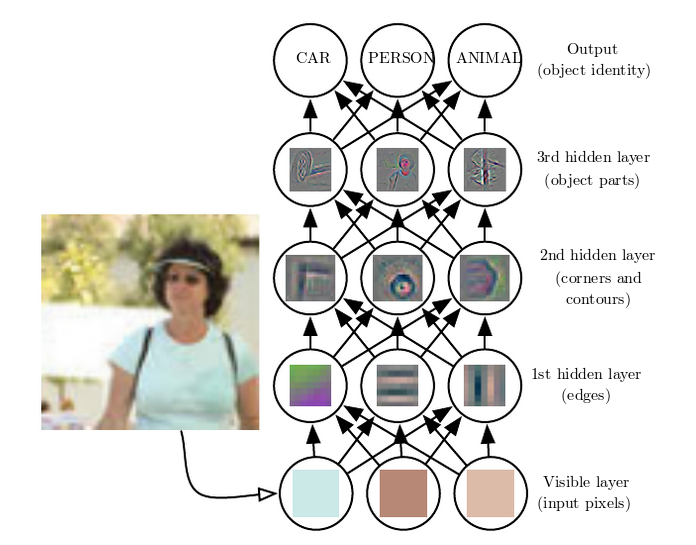
\includegraphics[width=\textwidth]{deep_learning_example}
		\caption{Hình mô phỏng cách hoạt động của mô hình học sâu cho bài toán nhận diện đối tượng trong ảnh.
		Dữ liệu đầu vào là hình ảnh RGB chứa đối tượng cần xác định. Tầng đầu tiên của mô hình là tầng ``input'' tiếp nhận thông tin này dưới dạng ma trấn số. 
		Các tầng tiếp theo ngoại trừ tầng cuối cùng được gọi là tầng ẩn ``hidden layer'' vì đặc trưng học được tại đây con người không quan sát được. 
		Các tầng ẩn học các đặc trưng ngày càng trừu tượng dựa vào đặc trưng ở tầng phía trước. 
		Tầng ẩn đầu tiên học được các đặc trưng về cạnh bằng cách so sánh độ sáng giữa các điểm ảnh gần nhau. 
		Tầng ẩn thứ hai học được các đặc trưng về đường cong bằng cách tổng hợp đặc trưng về cạnh ở tầng trước đó. 
		Tầng ẩn thứ ba học được các đặc trưng về bộ phận của đồ vật như khuôn mặt, bánh xe... dựa vào các đặc trưng về đường cong ở tầng trước. 
		Tầng cuối cùng được gọi là tầng ``output'' có nhiệm vụ tìm kiếm các bộ phận và trả về lớp đối tượng tương ứng. 
		Bằng cách học đặc trưng ngày càng trừu tượng hơn, các mô hình học sâu có khả năng tự động học được các đặc trưng từ đơn giản đến phức tạp; tất cả đều nhằm hỗ trợ cho quá trình phân lớp dữ liệu (hình được chỉnh sửa từ \cite{Goodfellow-et-al-2016-Book})}
		\label{dlex}
	\end{figure}
	
\subsection{Áp dụng học sâu để xấp xỉ hàm giá trị}
	Sức mạnh của các mô hình học sâu hoàn toàn có thể tận dụng vào bài toán học tăng cường.
	Cụ thể với những thuật toán học tăng cường được đề cập ở chương 2, việc xấp xỉ hàm giá trị là rất quan trọng.
	Chính vì vậy, một cách đơn giản nhất, ta có thể sử dụng các mô hình học sâu để xấp xỉ hàm giá trị.
	Một trong những mô hình tiêu biểu của học sâu đó là mạng nơ-ron (Neural networks).
	Việc sử dụng mạng nơ-ron để xấp xỉ hàm giá trị mang lại ba lợi ích quan trọng:
	\begin{itemize}
		\item Mạng nơ-ron có khả năng học được những đặc trưng phức tạp từ dữ liệu thô.
		\item Mạng nơ-ron có thể xấp xỉ hàm giá trị phức tạp.
		\item Mạng nơ-ron có tính tổng quát hoá.
	\end{itemize}
	
	Mạng nơ-ron là một mô hình học sâu nên có thể học được những đặc trưng phức tạp từ dữ liệu thô như đã nói ở phần trên.
	Cụ thể hơn trong bài toán tự động chơi game, ta có thể đưa dữ liệu đầu vào là các ``frame hình'' RGB thẳng vào ``input'' của mạng nơ-ron để tính ra giá trị tương ứng.
	Nhờ vậy, ta không cần phải thiết kế các đặc trưng bằng tay để biễu diễn cho từng trạng thái của game.
	Ngoài ra, do qua trình học đặc trưng là hoàn toàn tự động, thuật toán học tăng cường lúc này có thể áp dụng cho bất kỳ game nào mà không cần phải thay đổi cách rút trích đặc trưng.
	Với một mô hình cố định lúc này, ta có thể học chơi được nhiều game.
	Đây cũng chính là mục đích của bài toán tự động chơi game: xây dựng mô hình có khả năng tự động học chơi \textit{tốt} nhiều game chứ không chỉ chơi \textit{``hoàn hảo''} một game.
	
	Với bài toán tự động chơi game, giá trị của một trạng thái bất kỳ rất khó xác định do một màn game thường rất dài.
	Vì thế, hàm giá trị của bài toán này là một hàm phi tuyến phức tạp và không liên tục.
	Công cụ xấp xỉ hàm giá trị phải có khả năng xấp xỉ những hàm phức tạp như vậy thì thuật toán học tăng cường mới đạt được hiệu quả.
	Với cách nhìn nhận mạng nơ-ron như là một công cụ xấp xỉ hàm, ta có thể thấy mạng nơ-ron rất linh hoạt với khả năng xấp xỉ hàm đích bất kỳ.
	
	Một tính chất quan trọng khác của mạng nơ-ron chính là \textbf{khả năng tổng quát hoá} (Generalization).
	Nhờ đặc điểm này mà quá trình học tăng cường được tăng tốc đáng kể.
	Thay vì phải duyệt qua từng trạng thái (thậm chí phải duyệt nhiều lần) để tính hàm giá trị tại đó, mạng nơ-ron có khả năng ``dự đoán'' giá trị của một trạng thái chưa từng thấy dựa vào những trạng thái đã thấy.
	Như trong bài toán tự động chơi game thì các ``frame hình'' liên tiếp thường rất giống nhau và các trạng thái này thường cũng có giá trị tương đương nhau.
	Vì vậy, khi học xong cách chơi một game nào đó, thuật toán học tăng cường vẫn hoạt động tốt trong quá trình kiểm thử khi gặp những tình huống game chưa từng thấy trong lúc huấn luyện.
	
	Các thuật toán học tăng cường ở chương 2 đều lưu hàm giá trị dưới dạng bảng (lookup table).
	Để sử dụng mạng nơ-ron như một công cụ xấp xỉ hàm, lúc này ta coi hàm giá trị là một hàm có tham số (parameterized function) và đi tìm các tham số này:
	\begin{align}
		\hat{v}(s;\theta) &\approx v_{\pi}(s)\\
		\hat{q}(s,a;\theta) &\approx q_{\pi}(s,a)
		\label{eq_DefVhatQhat}
	\end{align}
	$\theta$ là bộ trọng số của mạng nơ-ron mà ta cần học.
	Để học được bộ trọng số xấp xỉ tốt hàm đích ($v_{\pi}(s)$ hoặc $q_{\pi}(s,a)$), ta cung cấp các mẫu dữ liệu (data sample).
	Mỗi mẫu bao gồm dữ liệu đầu vào của mạng nơ-ron (tức trạng thái $s$ hoặc bộ trạng thái, hành động $s, a$) cùng với giá trị đích mong muốn (tức $v_{\pi}(s)$ hoặc $q_{\pi}(s,a)$).
	Khi ta cung cấp đủ nhiều mẫu dữ liệu cho mạng nơ-ron, các bộ tham số sẽ được thay đổi để mạng xấp xỉ được hàm đích mong muốn.
	Số lượng mẫu dữ liệu càng lớn thì mạng nơ-ron càng ``thấy'' được nhiều giá trị tại nhiều vị trí khác nhau của hàm đích hơn, khi đó mạng nơ-ron càng có khả năng xấp xỉ hàm đích tốt hơn.	
	Để xét xem mạng nơ-ron có xấp xỉ tốt hàm đích hay chưa, ta có thể tính độ ``khác biệt'' của giá trị đích với giá trị xấp xỉ trên cả không gian đầu vào:
	\begin{align}
		J(\theta) &= \mathbb{E}_{s \sim \pi}[(v_{\pi}(s) - \hat{v}(s;\theta))^2]\\
		J(\theta) &= \mathbb{E}_{s,a \sim \pi}[(q_{\pi}(s,a) - \hat{q}(s,a;\theta))^2]
		\label{eq_ExpectedError}
	\end{align}
	Kỳ vọng $\mathbb{E}_{s \sim \pi}$ ý chỉ kỳ vọng với biến ngẫu nhiên là trạng thái $s$ được lấy từ phân bố do chính sách $\pi$ tạo nên.
	Ví dụ như ta cần xấp xỉ hàm giá trị của một chính sách chỉ luôn ``đi qua trái'' thì $s$ sẽ là những trạng thái mà khi đi theo chính sách này, ta có thể gặp được $s$.
	Trong khi đó nếu chính sách đang xét là ``đứng yên'' (không thay đổi trạng thái) thì $s$ chỉ có thể có một trạng thái duy nhất đó là trạng thái bắt đầu.
	Giá trị nằm trong kỳ vọng là độ lỗi bình phương giữa giá trị xấp xỉ và giá trị đích.
	Với hàm lỗi bình phương, có thể thấy khi $J(\theta)$ càng nhỏ thì bộ trọng số $\theta$ giúp cho mạng nơ-ron xấp xỉ hàm đích càng tốt.
	Lý do chính ta chọn độ lỗi bình phương (ví dụ thay vì độ lỗi theo trị tuyệt đối) là vì việc tính toán (như đạo hàm) trên hàm bình phương khá dễ dàng.
	
	Lưu ý là ở đây, hàm lỗi $J(\theta)$ là hàm theo $\theta$; tức là lúc này, ta cố định bộ trọng số $\theta$ để tìm ra ``sai số'' mà bộ trọng số này gây ra.
	Nếu ta có hai bộ trọng số $\theta_1$ và $\theta_2$, ta có thể so sánh khả năng xấp xỉ hàm đích của chúng bằng cách so sánh giá trị $J(\theta_1)$ và $J(\theta)_2$ tương ứng.
	
	Tuy nhiên ta không thể tính độ lỗi trên mọi điểm dữ liệu đầu vào theo công thức (\ref{eq_ExpectedError}) được vì số lượng trạng thái là rất lớn.
	Vậy ta có thể xấp xỉ giá trị $J(\theta)$ bằng cách chỉ xét độ lỗi trên một ``tập huấn luyện'' (hay còn gọi là ``Batch'') các trạng thái mà ta biết được giá trị đích.
	Khi đó, kỳ vọng $\mathbb{E}_{s \sim \pi}$ được thay thế bằng giá trị trung bình độ lỗi trên từng mẫu dữ liệu của ``batch'':
	\begin{align}
		J(\theta) &= \frac{1}{N} \sum_{i = 1}^{N}[(v_{\pi}(s_{i}) - \hat{v}(s_{i};\theta))^2]\\
		J(\theta) &= \frac{1}{N} \sum_{i = 1}^{N}[(q_{\pi}(s_i,a_i) - \hat{q}(s_i,a_i;\theta))^2]
		\label{eq_BatchError}
	\end{align}
	Trong đó:
	\begin{itemize}
		\item N là số mẫu dữ liệu trong ``batch''.
		\item $s_i$, $a_i$ tương ứng là trạng thái và hành động của mẫu dữ liệu thứ $i$ của ``batch''.
	\end{itemize}
	Với một tập huấn luyện bất kỳ (tức một ``batch''), ta mong muốn tìm được bộ trọng số giúp cho mạng nơ-ron xấp xỉ tốt hàm đích trên các mẫu dữ liệu thuộc tập huấn luyện này.
	Một thuật toán đơn giản và hay được sử dụng để tìm bộ trọng số này đó là ``Batch Gradient Descent'' (BGD).
	Để cực tiểu hoá hàm $J(\theta)$, thuật toán BGD thực hiện lặp lại nhiều ``bước đi'' nhỏ để thay đổi bộ trọng số $\theta$ dần dần; mỗi bước đi sẽ giúp cho hàm $J(\theta)$ giảm đi một ít.
	Để chọn ``hướng đi'' (tức cách cập nhật $\theta$) thì BGD sẽ ``nhìn'' xung quanh vị trí hiện tại và đi theo hướng nào giúp giảm $J(\theta)$ nhiều nhất có thể.
	
	
	Tuy nhiên, giá trị đích thực sự mà ta mong muốn là $v_{\pi}(s)$ (hoặc $q_{\pi}(s,a)$) ta không hề biết.
	Các thuật toán học tăng cường chính là kỹ thuật giúp ta có được một ước lượng đơn giản của giá trị đích này.
	

%\begin{itemize}
%	\item Lý do kết hợp học sâu với học tăng cường
%	\item Giới thiệu học sâu
%	\item Áp dụng học sâu để xấp xỉ hàm giá trị
%	\item Giới thiệu mạng ``Convolutional Neural Network''
%\end{itemize}
	
\section{Học tăng cường sâu}
%\begin{itemize}
%	\item Cấu trúc mạng ``Deep Q-Networks'' cho bài toán tự động chơi game
%	\item Kỹ thuật làm tăng tính ổn định cho quá trình học
%	\begin{itemize}
%		\item Học từ dữ liệu trong quá khứ ``Experience replay''
%		\item Cố định hàm giá trị đích ``Fixed Q-targets''
%	\end{itemize}
%\end{itemize}
%	
%\section{Đề xuất phương pháp cải tiến (Nếu có)}
	
	\chapter{Kết quả thực nghiệm}
\ifpdf
\graphicspath{{Chapter4/Chapter4Figs/PNG/}{Chapter4/Chapter4Figs/PDF/}{Chapter4/Chapter4Figs/}}
\else
\graphicspath{{Chapter4/Chapter4Figs/EPS/}{Chapter4/Chapter4Figs/}}
\fi
\begin{quote}
	\textit{Trong chương này, chúng em trình bày kết quả thực nghiệm của bài toán tự động chơi game.
	Đầu tiên, môi trường giả lập của bài toán tự động chơi game cùng với các thiết lập thực nghiệm được giới thiệu.
	Phần tiếp theo, chúng em trình bày về kết quả thực nghiệm của thuật toán ``Q-learning'' để chứng minh tính khả thi của việc kết hợp học tăng cường với học sâu vào bài toán tự động chơi game.
	Kế tiếp, chúng em phân tích mức độ ảnh hưởng của vấn đề ``đánh giá quá cao'' và kết quả của thuật toán ``Double Q-learning''.
	Phần cuối cùng bao gồm một số thực nghiệm chứng minh rằng mô hình mạng nơ-ron xấp xỉ tốt hàm giá trị hành động.}
\end{quote}
 
\section{Giới thiệu Arcade Learning Environment}
Arcade Learning Environment (ALE) là một framework được thiết kế giúp dễ dàng trong việc phát triển những hệ thống có thể tự động chơi bất kỳ những game trên hệ máy Atari 2600.
\subsection{Hệ máy Atari 2600}
\ref{fig:AtariConsole} là hệ máy chơi game Atari 2600 tại gia đình được phát triển và sử dụng phổ biến vào những năm 1970.
Hơn 500 game đã được phát triển cho hệ máy này; một số game vẫn tiếp tục được phát triển cho tới ngày nay. 
Độ phân giải của những game này là $210 \times 160$. 
Mặc dù vậy nhiều game được phát triển cho hệ máy này, nhưng cấu hình phần cứng của chúng khá đơn giản bao gồm một CPU 1.19 Mhz, một bộ nhớ ROM 2-4KB để lưu giữ code của game, và dung lượng RAM của máy cũng chỉ là 128 bytes. 
Đồ họa của các game được cố định ở độ phân giải $160 x 210$, với ảnh màu RGB. 
Người chơi tương tác với game qua một thiết bị được gọi là joystick, có thể thực hiện tối đa 18 hành động.

\subsection{Interface}
ALE được xây dựng trên nền Stella, nó giả lập máy hệ máy Atari 2600. Qua đó cho phép người dùng tương tác với Atari 2600 bằng cách tiếp nhận những di chuyển của joystick, gửi thông tin của game cho người dùng như hình ảnh, điểm số nhận được. 
ALE cũng cung cấp một \textit{lớp sử lý} để chuyển đổi những thông tin trong game theo chuẩn của bài toán học tăng cường như điểm số đạt được, kết thúc game chưa. 
Mặc định, lớp này biểu diễn mỗi trạng thái trong game bằng một mảng 7-bit pixels 2 chiều, và không gian hành động gồm 18 hành động tương ứng với các hành động có thể thực hiện trong joystick. 
Lớp sử lý cung cấp thông tin tập những hành động cụ thể có thể thực hiện trong một game. 
ALE có thể tạo ra 60 frame hình ảnh game trong một giây theo mặc định, và số frame ảnh nhiều nhất trong một giây nó có thể tạo ra 6000 frame. 
Điểm số nhận được tại từng thời điểm được định nghĩa theo từng game khác nhau. 
Một mẫu thực nghiệm có thể được tao ra từ frame đầu tiên của game cho đến khi game kết thúc, ngoài ra lớp sử lý cũng cho phép người người tạo mãu thực nghiệm với số lượng frame cố định.

ALE hơn nữa cũng cung cấp chức năng \textit{sao lưu} và \textit{khôi phục} trạng thái của game. 
Khi lệnh sao lưu được thực thi, ALE lưu lại tất cả các dữ liệu liên quan tại thời điểm đó trong game như nội dung RAM, registers. 
Ngược lại khi lệnh khôi phục được thực thi, nó sẽ khởi tạo lại trạng thái game đã lưu lại trước đó.

\begin{figure}
	\centering
	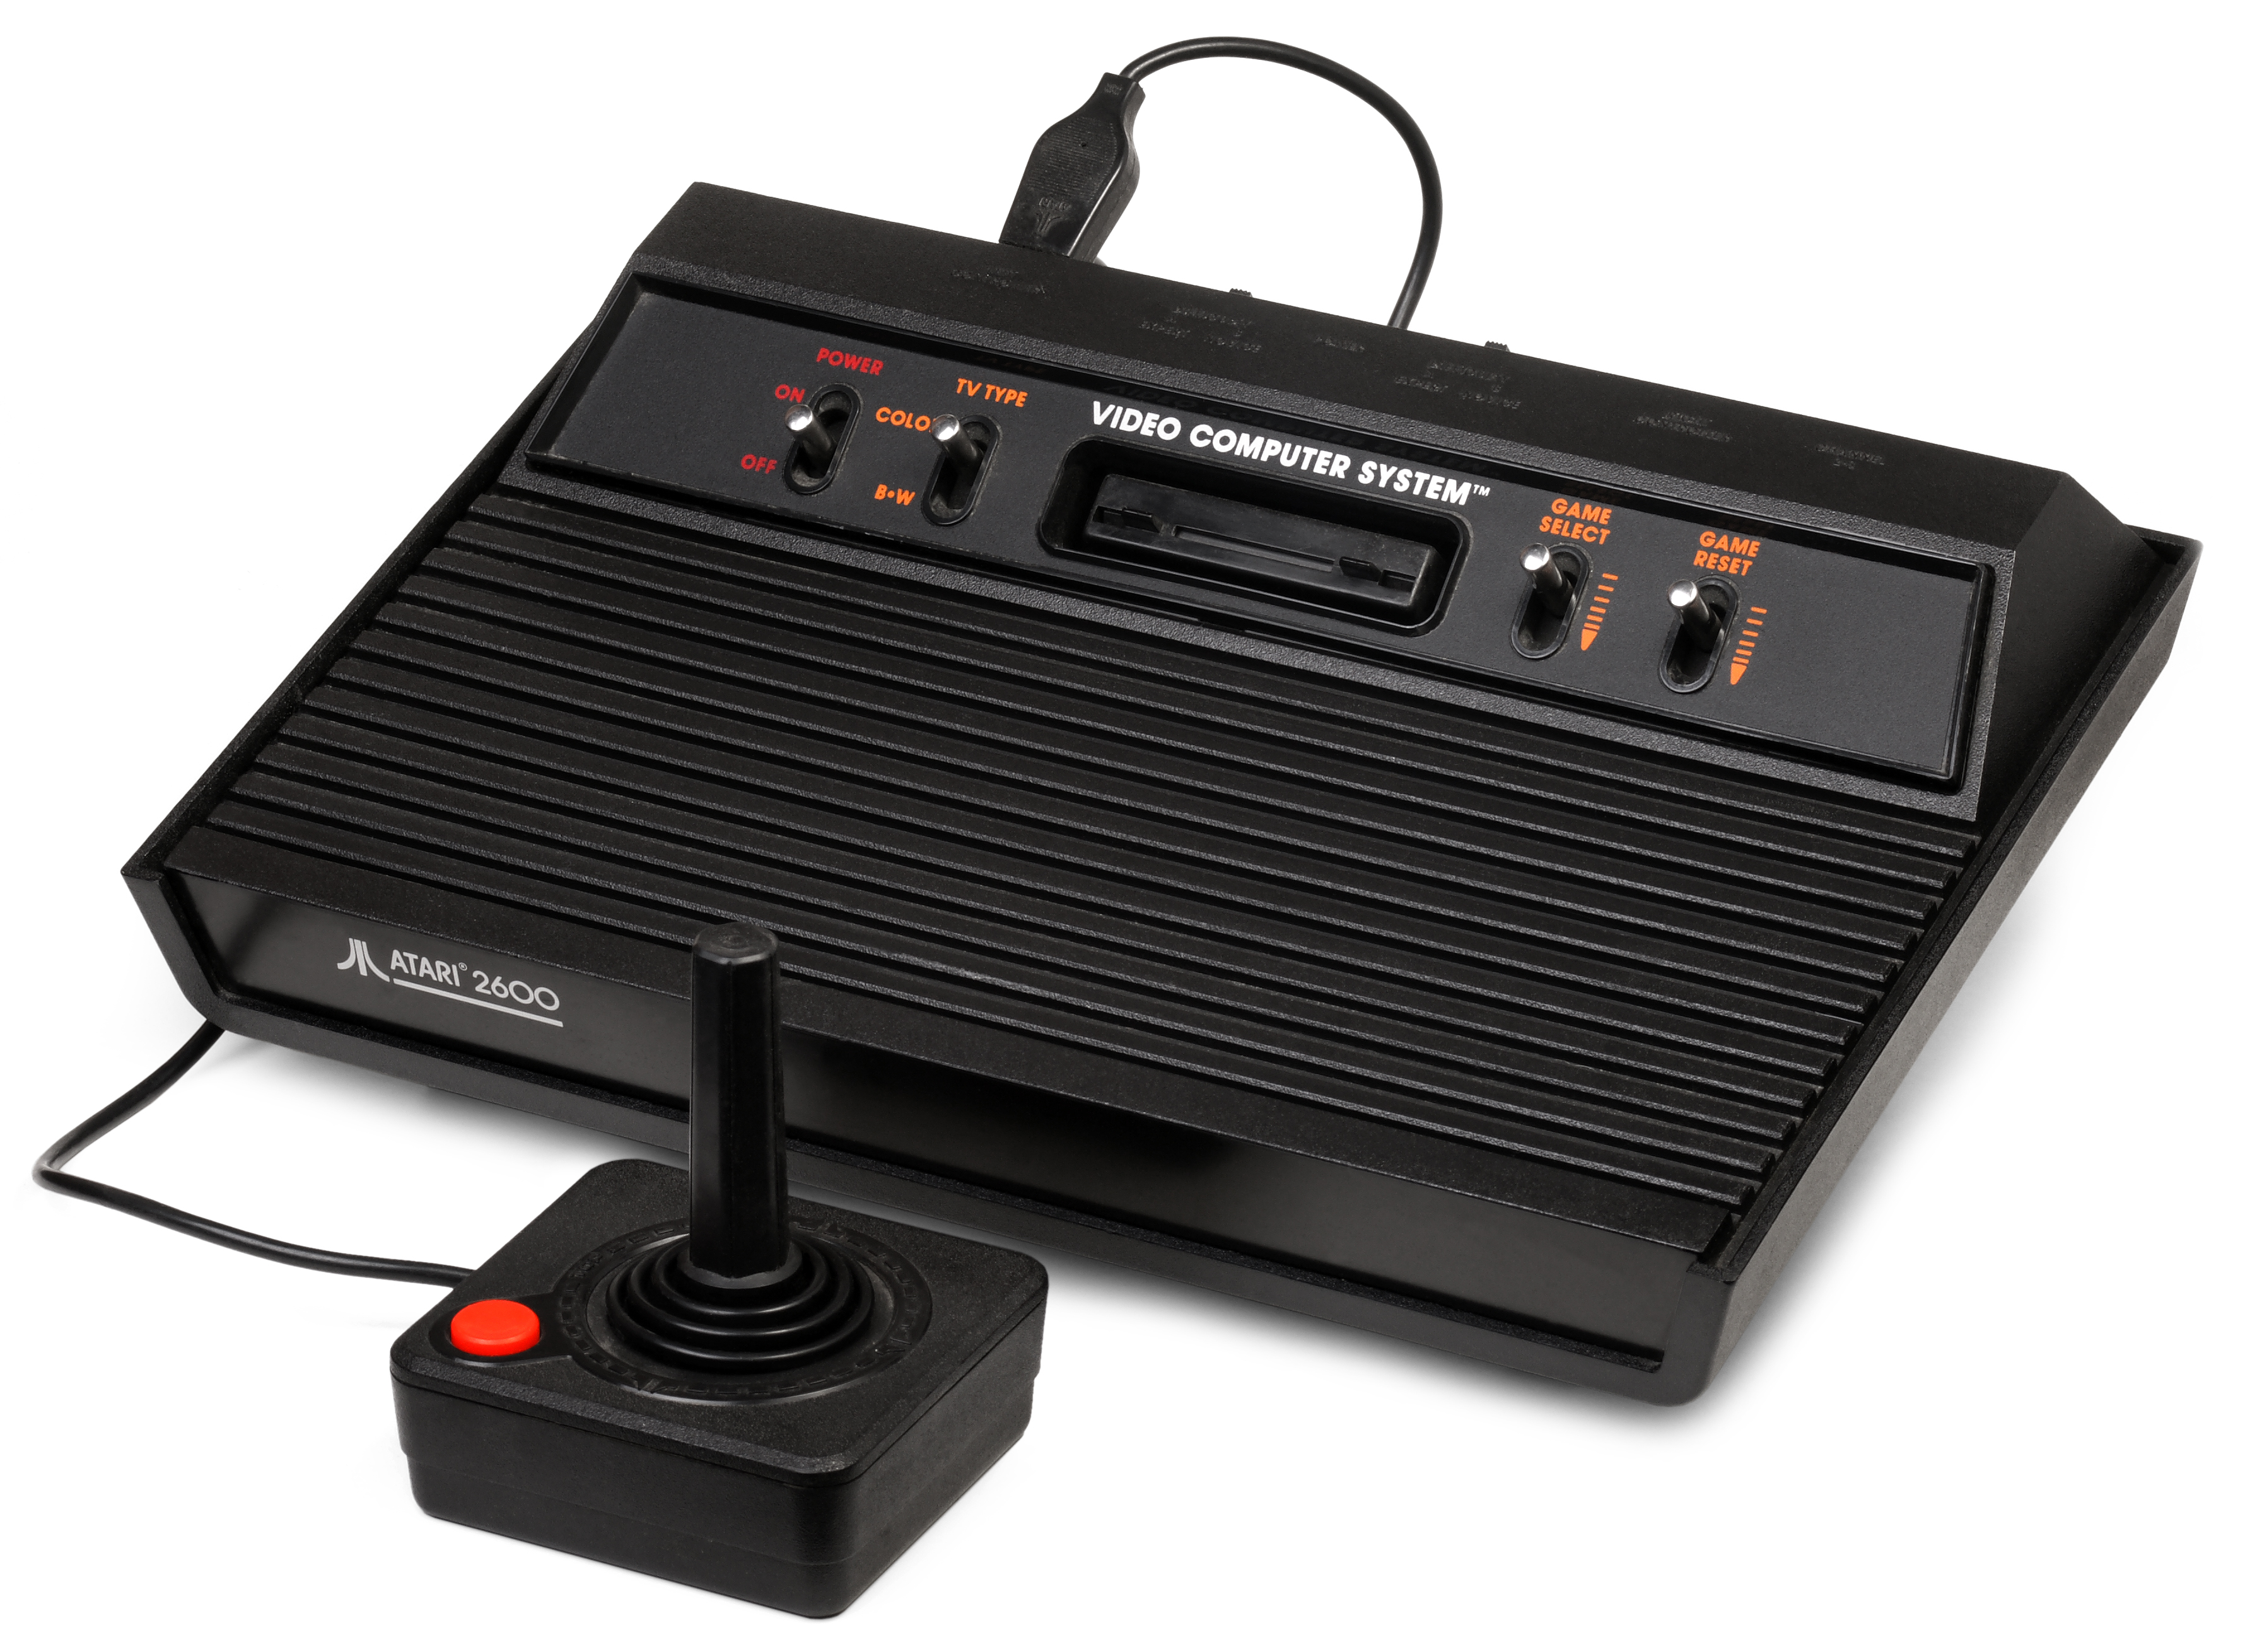
\includegraphics[width=90mm]{Atari2600Console.jpg}
	\caption{Hệ máy chơi game Atari 2600}
	\label{fig:AtariConsole}
\end{figure}

\section{Các thiết lập thực nghiệm}
	Chúng em thực hiện huấn luyện hệ thống trên ba trò chơi: \textit{Assault}, \textit{Breakout} và \textit{Seaquest}.
	Việc thực nghiệm trên ba trò chơi là để chứng minh hướng tiếp cận kết hợp học sâu với học tăng cường có thể áp dụng vào nhiều trò chơi khác nhau.
	\textit{Assault} là trò chơi bắn máy bay truyền thống: hệ thống điều khiển máy bay bay qua trái, phải hoặc bắn tên lửa để hạ máy bay địch.
	\textit{Breakout} là trò chơi ``phá gạch'': hệ thống điều khiển một mái chèo (paddle) qua trái, phải để giữ cho trái banh không rơi xuống dưới; phía trên là những viên gạch bị phá huỷ và cho điểm thưởng khi chạm phải trái banh.
	Cuối cùng là trò chơi \textit{Seaquest} có nội dung tương tự như ``Assault'' nhưng là điểu khiển tàu ngầm theo cả tám hướng xung quanh.
	Tuy các trò chơi này có nội dung tương tự nhau nhưng luật chơi cụ thể lại rất khác biệt và đòi hỏi chiến thuật mang tính ``dài hơi''.
	Ví dụ như màn hình trò chơi \textit{Seaquest} có một thanh không khí thể hiện mức độ không khí còn lại trong tàu ngầm.
	Khi thanh này cạn thì ta cần điều khiển tàu ngầm nổi lên mặt nước để lấy không khí.
	Vì vậy, hệ thống cần học được đặc trưng thể hiện mức không khí còn lại và dựa vào đó để điều khiển tàu ngầm nổi lên mặt nước.
	Ngoài ra, để chơi tốt và đạt nhiều điểm, hệ thống cần học được chiến thuật đợi không khí còn lại ít nhất rồi mới nổi lên mặt nước một lần để tiết kiệm thời gian.
	Ví dụ này cho thấy các trò chơi này đều đòi hỏi các đặc trưng học được phải rất trừu tượng và chiến thuật chơi cũng phải khá phức tạp.
	Hình () thể hiện màn hình một khung ảnh của ba trò chơi trên.
	
	Để giảm bớt tính toán của mô hình, khung ảnh RGB đầu vào được chuyển về ảnh mức xám (grayscale) và được giảm kích thước về $84\times84$.
	Để lưu thông tin về sự di chuyển và tốc độ của các đối tượng trong ảnh, ta ghép bốn khung ảnh liên tiếp nhau lại thành một trạng thái.
	Vậy một trạng thái lúc này sẽ gồm bốn ảnh mức xám $84\times84$ và được đưa trực tiếp vào ``input'' của mạng nơ-ron.
	Ngoài ra, do các khung hình gần nhau thường không thay đổi nhiều, một kỹ thuật đơn giản để tăng tốc độ huấn luyện đó là ta lặp lại một hành động cho $k$ khung hình liên tiếp.
	Nhờ kỹ thuật này, ta có thể huấn luyện nhiều hơn $k$ lần so với khi không áp dụng.
	Trong thực nghiệm này, chúng em chọn $k$ bằng 4 theo đề xuất của (\cite{mnih2013playing}).
	
	Cấu trúc mạng nơ-ron tích chập được dùng để xấp xỉ hàm giá trị là ``Deep Q-Network'' (\cite{mnihdqn2015}).
	Mạng này bao gồm bốn tầng ẩn với ba tầng đầu là tầng tích chập và tầng cuối là tầng ``Fully-connected''.
	Tầng tích chập đầu tiên gồm $32$ bộ lọc với kích thước $8\times8$ và bước dịch chuyển (stride) là $4\times4$.
	Tầng tích chập thứ hai gồm $64$ bộ lọc với kích thước $4\times4$ và bước dịch chuyển là $2\times2$.
	Tầng tích chập cuối cùng gồm $64$ bộ lọc với kích thước $3\times3$ và bước dịch chuyển là $1\times1$.
	Đầu ra của tầng tích chập được đưa vào một tầng ``Fully-connected'' gồm $512$ nơ-ron ẩn để tổng hợp đặc trưng.
	Tầng ``output'' của mạng cũng là một tầng ``Fully-connected'' với số nơ-ron ẩn là số hành động của trò chơi (6 cho ``Assault'', 4 cho ``Breakout'' và 18 cho ``Seaquest'').
	Tầng này sẽ trả về giá trị hành động tương ứng cho trạng thái đầu vào.
	Hàm kích hoạt của tất cả các tầng ẩn là hàm ``Rectified'': $\sigma(x) = \max(0, x)$.
	
	Để huấn luyện mạng nơ-ron này, chúng em áp dụng thuật toán ``RMSprop'' (\cite{tieleman2012lecture}) để tối tiểu hàm lỗi bình phương.
	Đây là một thuật toán cải tiến của SGD với ý tưởng chọn một hệ số học khác nhau cho từng trọng số của mạng nơ-ron.
	Hệ số học của mỗi trọng số sẽ phụ thuộc vào giá trị đạo hàm của hàm lỗi đối với trọng số này ở các bước cập nhật trước.
	Cụ thể hơn, nếu trọng số này được cập nhật ít ở những lần cập nhật trước thì hệ số học sẽ được tăng lên; trọng số được cập nhật nhiều thì sẽ có hệ số học giảm đi.
	Nhờ thuật toán này mà mức độ thay đổi của các trọng số là tương đương nhau.
	
	Chúng em sử dụng ``Python'' (kết hợp với framework ``Theano'' (\cite{2016arXiv160502688short})) làm ngôn ngữ lập trình chính.
	Do việc huấn luyện đòi hỏi sức mạnh tính toán rất lớn nên chúng em thực hiện cài đặt tính toán song song trên GPU để tăng tốc.
	GPU được dùng là NVIDIA GTX 980.
	
	Với các thiết lập thực nghiệm trên, chúng em tiến hành huấn luyện ba trò chơi với hai thuật toán ``Q-learning'' và ``Double Q-learning''.
	Mỗi trò chơi với mỗi thuật toán được huấn luyện $50$ triệu hành động.
	Thời gian huấn luyện là khoảng 50 giờ cho mỗi trò chơi với mỗi thuật toán.
	
\section{Thuật toán ``Q-learning''}
	Để thực nghiệm khả năng học và tự động chơi game, chúng em thực hiện thử nghiệm thuật toán ``Q-learning'' kết hợp với học sâu.
	Chúng em sử dụng chính sách $\epsilon$-greedy để làm chính sách khám phá không gian trạng thái và không gian hành động.
	$\epsilon$-greedy được chọn ở đây là vì chính sách này đơn giản cho việc cài đặt mà vẫn đảm bảo khả năng khám phá không gian cũng như khai thác kiến thức đã học của mô hình.
	Do ban đầu hệ thống chưa có nhiều hiểu biết về môi trường, chúng ta nên khám phá nhiều hơn; sau khi có một số hiểu biết nhất định thì hệ thống lại cần khai thác những hiểu biết đó.
	Ý tưởng này có thể dễ dàng được cài đặt bằng cách giảm dần hệ số $\epsilon$ trong khi đang huấn luyện.
	Với thuật toán ``Q-learning'', chúng em thực hiện giảm dần $\epsilon$ từ $1.0$ về $0.1$ trong $1$ triệu hành động đầu tiên.
	
	Để tiện cho việc quan sát kết quả và thử nghiệm hệ thống, chúng em chia quá trình huấn luyện $50$ triệu hành động ra thành $200$ ``epoch'' (tức mỗi ``epoch'' bao gồm $250000$ hành động).
	Sau mỗi ``epoch'', chúng em kiểm thử bộ trọng số học được trên $30$ màn chơi và lưu lại điểm số trung bình.
	Kết quả điểm số cuối cùng được báo cáo của mỗi trò chơi là giá trị điểm số lớn nhất của $200$ epoch.
	Các thiết lập trên tương đồng với (\cite{mnihdqn2015}) để việc so sánh là công bằng nhất.
	
	Một đặc điểm của bài toán tự động chơi game đó là kết quả điểm thưởng sau từng ``epoch'' thường rất nhiễu.
	Giá trị của các trọng số mạng nơ-ron có thể thay đổi ít sau mỗi ``epoch'' nhưng hàm giá trị tương ứng sẽ thay đổi nhiều.
	Điều này dẫn đến chính sách tương ứng cũng thay đổi nhiều làm cho điểm thưởng nhận được khi chơi game của các chính sách này sẽ rất khác nhau.
	Vì vậy nếu ta chỉ quan sát đồ thị điểm thưởng của quá trình kiểm thử sau mỗi ``epoch'', ta sẽ không biết chắc là hệ thống có đang chơi tốt lên hơn không.
	Một cách khác để quan sát quá trình học được đề xuất bởi (\cite{mnih2013playing}) đó là ta quan sát đồ thị giá trị của một tập trạng thái sau từng ``epoch''.
	Đầu tiên, ta thực hiện chơi game một cách ngẫu nhiên và lưu lại một tập các trạng thái gặp được trong quá trình chơi này (gọi là tập ``hold-out'').
	Trong quá trình huấn luyện, sau mỗi ``epoch'', ta tính trung bình giá trị hành động tốt nhất của các trạng thái trong tập ``hold-out''.
	Một chính sách chơi tốt thì thường sẽ đánh giá các hành động của các trạng thái trong tập ``hold-out'' cao hơn so với các chính sách chơi không tốt.
	Vì vậy, quan sát đồ thị này là một cách đơn giản để theo dõi quá trình học của hệ thống.
	\begin{figure}
		\centering
		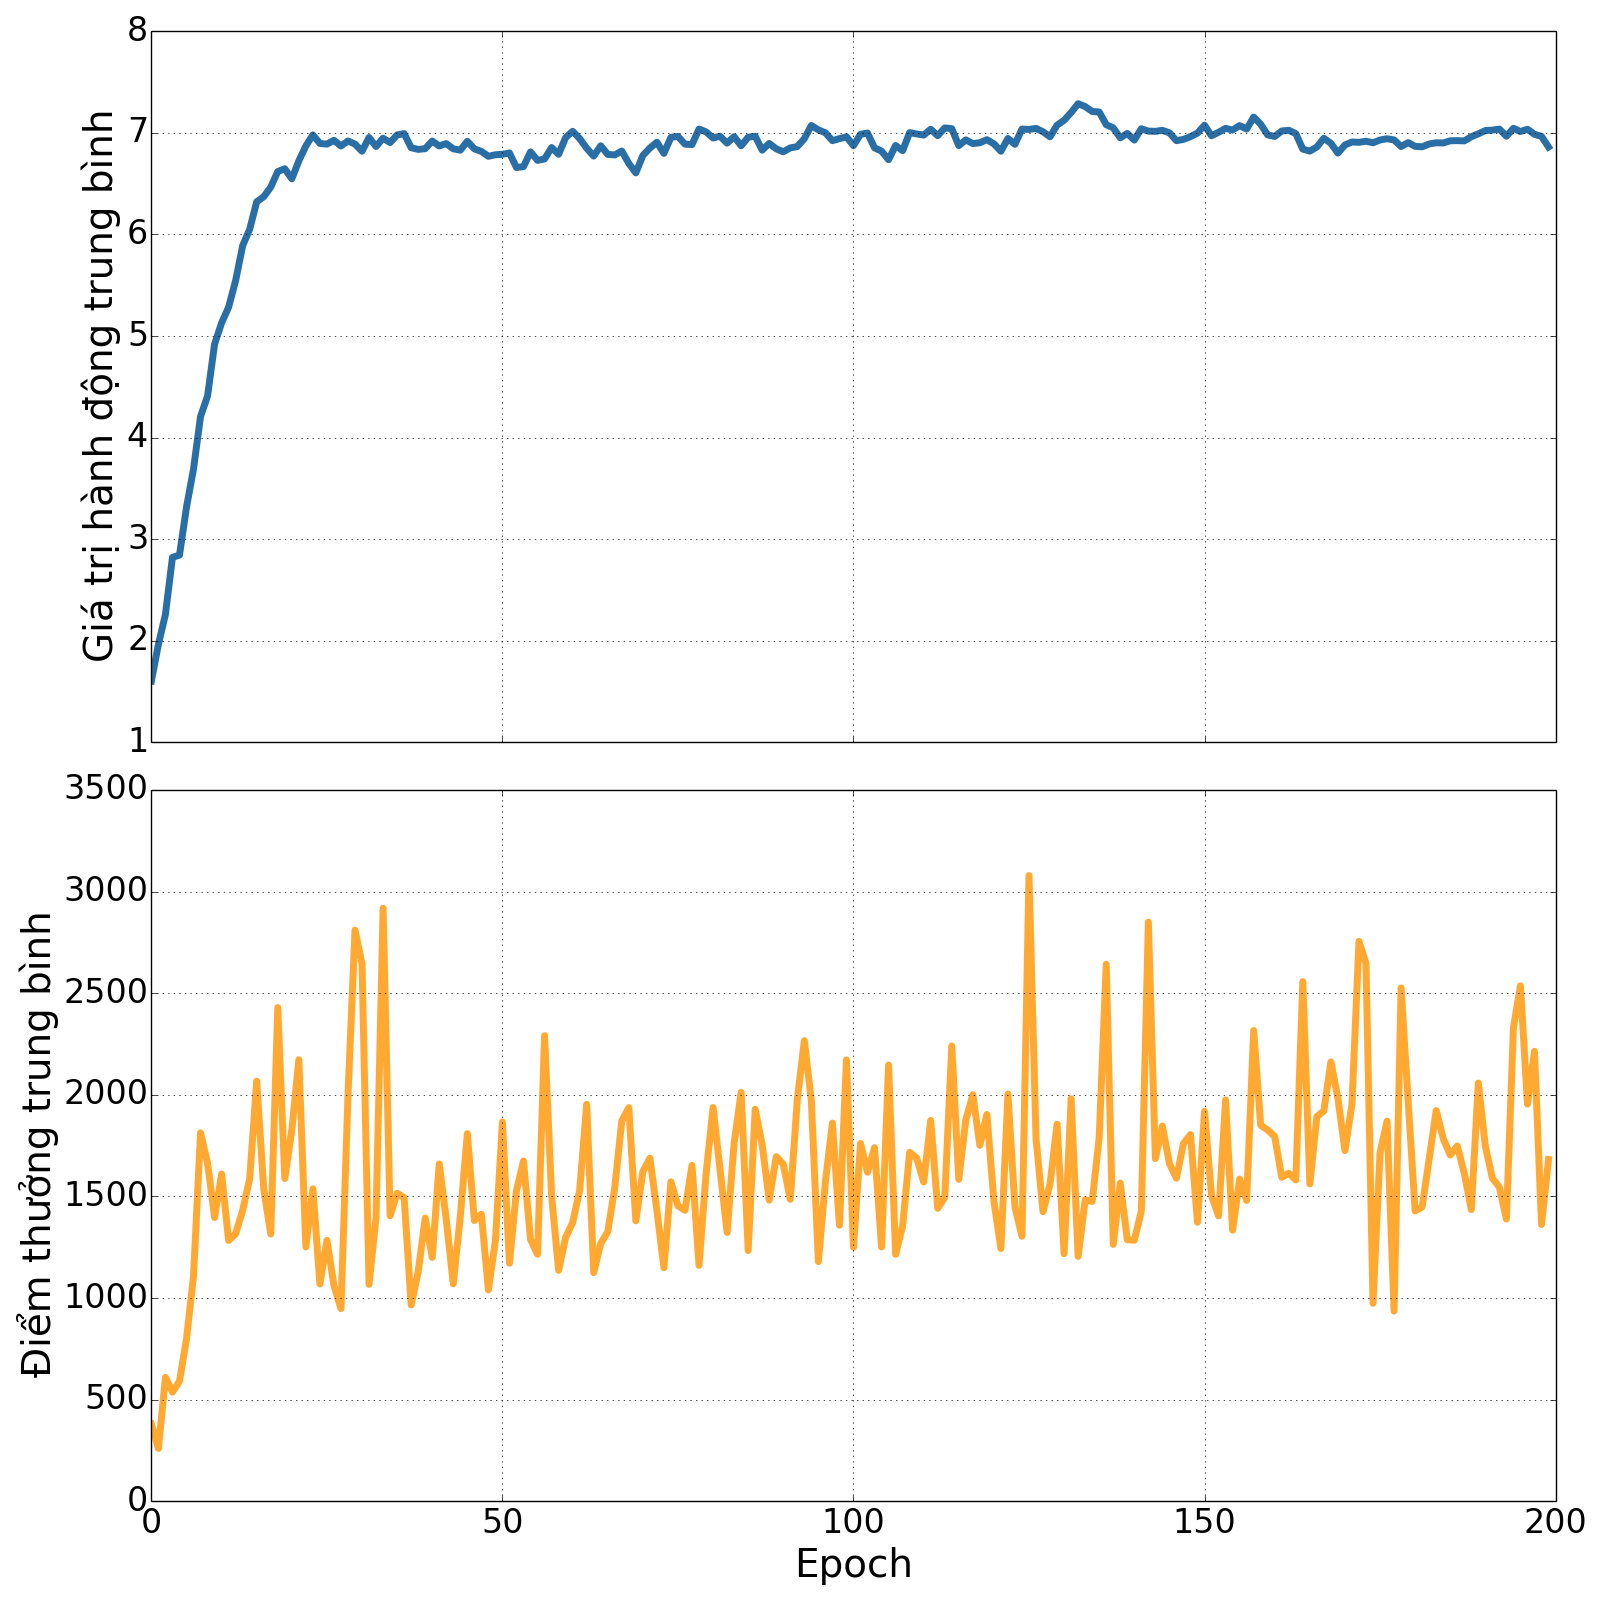
\includegraphics[width=\textwidth]{dqn_assault_values_rewards}
		\caption[Đồ thị giá trị hành động trung bình và điểm thưởng trung bình]{
		Đồ thị kết quả của trò chơi \textit{Assault}. 
		Đồ thị ở trên thể hiện trung bình giá trị hành động trên tập ``hold-out'' theo ``epoch'' huấn luyện; đồ thị ở dưới thể hiện điểm thưởng trung bình theo ``epoch'' huấn luyện.
		Điểm thưởng trung bình thay đổi rất nhiều sau từng ``epoch''.
		Nếu sử dụng đồ thị này để theo dõi quá trình huấn luyện thì ta sẽ không biết là hệ thống có đang học được cách chơi game hay không.
		Trong khi đó, đồ thị giá trị hành động lại ít nhiễu hơn và hội tụ dần đến một mức nhất định.
		Quan sát đồ thị này, ta thấy những ``epoch'' đầu hệ thống học rất nhanh và sau khoảng $50$ ``epoch'' thì giá trị hành động không tăng cao hơn nữa.
		Lúc này, ta có thể dừng việc học sớm.
		Tuy nhiên, một số game có thể cần học lâu hơn.
		Vì vậy, chúng em cố định số ``epoch'' để huấn luyện được nhiều trò chơi mà không phải thay đổi siêu tham số.}
		\label{fig_assault_vr}
	\end{figure}
	
	Hình (\ref{fig_assault_vr}) thể hiện đồ thị điểm số và giá trị trạng thái trên tập ``hold-out'' của trò chơi \textit{Assault}.
	Điểm thưởng kết quả của ba game được báo cáo trong bảng (\ref{table_dqn_results}).
	Cả ba game được thực nghiệm cho kết quả vượt xa kết quả chơi ngẫu nhiên.
	Điều này cho thấy hệ thống thật sự học được cách chơi để đạt được nhiều điểm số dù ban đầu không hề biết quy luật chơi.
	Hai trong số ba game còn cho kết quả hơn cả kết quả do con người chơi.
	Tuy nhiên, bài báo \cite{mnihdqn2015} chỉ cho người chơi học thử khoảng 2 giờ cho mỗi game, ít hơn nhiều so với việc huấn luyện $50$ triệu hành động (tức khoảng 38 ngày chơi) của hệ thống.
	Vì vậy, điểm thưởng nhận được của con người trong bảng (\ref{table_dqn_results}) chỉ mang tính tham khảo.
	Dù chúng em thực hiện cài đặt lại thuật toán được đề xuất bởi bài báo \cite{mnihdqn2015} nhưng kết quả cũng không bằng nhau (cao hơn ở game \textit{Seaquest} và thấp hơn ở hai game còn lại).
	Lý do chính của điều này là vì cách cài đặt khác nhau và chương trình giả lập game Atari khác nhau.
	
	\begin{table}
		\centering
		\caption[Điểm thưởng nhận được của thuật toán ``Q-learning'']{
		Kết quả \textit{Ngẫu nhiên} nhận được bằng cách chơi với chính sách ngẫu nhiên (chọn hành động theo phân bố đều).
		Kết quả \textit{Con người} nhận được bằng cách cho một số người học và chơi các game này.
		\textit{Kết quả gốc} là kết quả thực nghiệm của bài báo \cite{mnihdqn2015}.
		Kết quả \textit{Thực nghiệm} là kết quả do nhóm thực hiện cài đặt lại thuật toán ``Q-learning''.
		Giá trị được in đậm là giá trị lớn nhất của mỗi dòng.}
		\label{table_dqn_results}
		\begin{tabular}{| l | c | c | c | c |}
			\hline
			 & \textit{Ngẫu nhiên}\cite{mnihdqn2015} & \textit{Con người}\cite{mnihdqn2015} & \textit{Kết quả gốc}\cite{mnihdqn2015} & \textit{Thực nghiệm} \\
			\hline \hline
			\textit{Assault} & 222.4 & 742.0 & \textbf{4,280.4} & 3,078.8 \\ 
			\hline
			\textit{Breakout} & 1.7 & 30.5 & \textbf{385.5} & 377.6 \\ 
			\hline
			\textit{Seaquest} & 68.4 & \textbf{42,054.7} & 5,860.6 & 6,340.7 \\ 
			\hline
		\end{tabular}		
	\end{table}

\section{Thuật toán ``Double Q-learning''}
	Chúng em thực hiện cài đặt và thử nghiệm lại thuật toán ``Double Q-learning'' \cite{hasselt2010double}, \cite{van2015deep} để giải quyết vấn đề đánh giá quá cao.
	Các thiết lập thực nghiệm đều giống như khi thực nghiệm thuật toán ``Q-learning''.
	Tuy nhiên, để tương đồng với cài đặt của bài báo \cite{van2015deep}, chúng em giảm hệ số $\epsilon$ từ $1.0$ xuống $0.01$ (thay vì $0.1$ như ở phần thực nghiệm ``Q-learning'') trong $1$ triệu hành động đầu tiên của quá trình huấn luyện.
	
	\begin{table}
		\centering
		\caption[Điểm thưởng nhận được của thuật toán ``Double Q-learning'']{
		Kết quả \textit{Ngẫu nhiên} và \textit{Con người} được trích từ bài báo \cite{van2015deep}.
		Do môi trường giả lập game khác nhau nên chúng em chỉ so sánh ``Double Q-learning'' với phiên bản cài đặt ``Q-learning'' của nhóm thay vì so sánh với phiên bản ``Double Q-learning'' của bài báo \cite{van2015deep}.
		Giá trị được in đậm là giá trị lớn nhất của mỗi dòng.}
		\label{table_double_results}
		\begin{tabular}{| l | c | c | c | c |}
			\hline
			 & \textit{Ngẫu nhiên}\cite{mnihdqn2015} & \textit{Con người}\cite{mnihdqn2015} & \textit{Q-learning} & \textit{Double Q-learning} \\
			\hline \hline
			\textit{Assault} & 222.4 & 742.0 & 3,078.8 & \textbf{4864.6} \\
			\hline
			\textit{Breakout} & 1.7 & 30.5 & 377.6 & \textbf{431.2} \\
			\hline
			\textit{Seaquest} & 68.4 & \textbf{42,054.7} & 6,340.7 & 13,186 \\
			\hline
		\end{tabular}		
	\end{table}
	
	Bảng \ref{table_double_results} cho biết kết quả của thuật toán ``Double Q-learning'' trên ba game.
	Thuật toán ``Double Q-learning'' cho kết quả tốt hơn hẳn điểm số của ``Q-learning'' trên cả ba game và cao hơn gấp đôi ở game \textit{Seaquest}.
	Lý do ``Double Q-learning'' hoạt động tốt như vậy trên game \textit{Seaquest} là vì game này có nhiều hành động (18 so với 4 của \textit{Breakout} và 6 của \textit{Assault}).
	Số lượng hành động càng nhiều thì khả năng bị đánh giá quá cao lại càng tăng.
	Vì vậy, thuật toán ``Q-learning'' bị ảnh hưởng rất lớn bởi vấn đề đánh giá quá cao và thuật toán ``Double Q-learning'' cho kết quả tốt hơn hẳn khi giải quyết được vấn đề này.
	Các kết quả này cho thấy thuật toán ``Double Q-learning'' là một cải tiến rất tốt cho bài toán tự động chơi game.
	
	Để thấy rõ hơn việc hạn chế vấn đề đánh giá quá cao của ``Double Q-learning'', ta có thể coi đồ thị giá trị hành động trung bình trên tập ``hold-out'' và đồ thị điểm thưởng trung bình của cả hai thuật toán ở hình (\ref{fig_double_compare}).
	Thuật toán ``Double Q-learning'' cho kết quả điểm thưởng tốt hơn hẳn ``Q-learning'' vì đánh giá hành động chính xác hơn (không bị vấn đề đánh giá quá cao).
	
	\begin{figure}
		\centering
		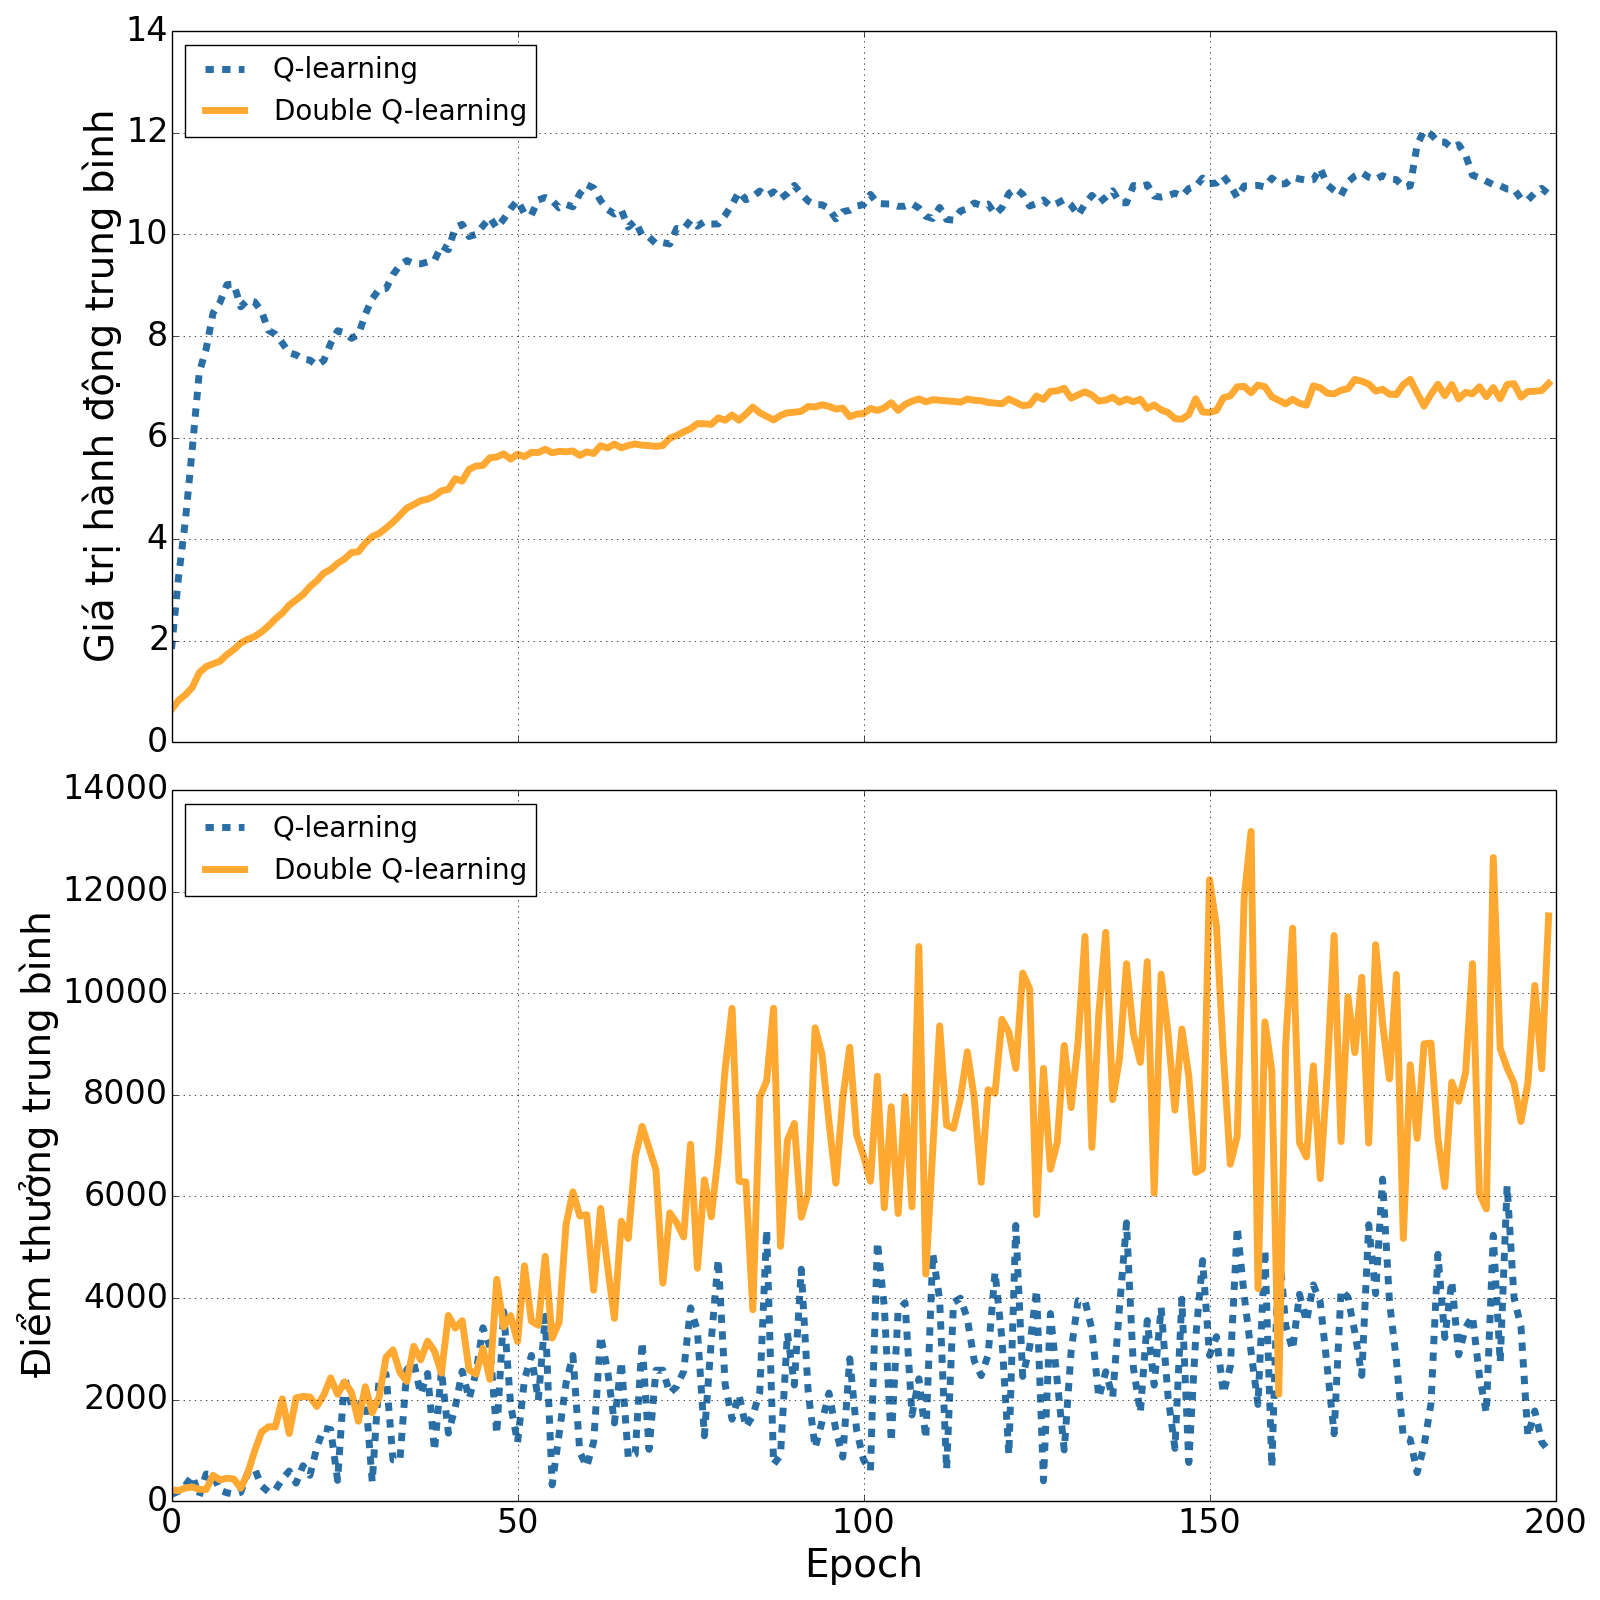
\includegraphics[width=\textwidth]{double_compare}
		\caption[Đồ thị giá trị hành động trung bình và điểm thưởng trung bình của hai thuật toán]{
		Đồ thị kết quả của trò chơi \textit{Seaquest}.
		Hình phía trên là đồ thị giá trị hành động trung bình theo ``epoch''; hình phía dưới là đồ thị điểm thưởng trung bình theo ``epoch''.
		Ở đồ thị phía trên, thuật toán ``Q-learning'' đánh giá rất cao các hành động của trạng thái thuộc tập ``hold-out''.
		Tuy nhiên, khi chơi thử game thì thuật toán ``Q-learning'' lại cho điểm thưởng rất thấp.
		Điều này cho thấy thuật toán ``Q-learning'' gặp vấn đề đánh giá quá cao và vấn đề này ảnh hưởng đến kết quả chơi game của hệ thống.
		Trong khi đó, thuật toán ``Double Q-learning'' tuy đánh giá các hành động của trạng thái thuộc tập ``hold-out'' thấp hơn nhưng khi chơi game thì lại được nhiều điểm thưởng hơn.
		Thuật toán ``Double Q-learning'' đánh giá chính xác hơn giá trị hành động và vì thế, chính sách chơi game cũng tốt hơn.}
		\label{fig_double_compare}
	\end{figure}
		
\section{Phân tích hàm giá trị hành động}
	Để thấy rõ hơn khả năng xấp xỉ hàm giá trị của mạng nơ-ron, ta có thể xem xét giá trị của một số trạng thái trong quá trình chơi game.
	Cụ thể hơn, chúng em thực hiện lưu một số ``frame'' ảnh trong quá trình chơi cùng với giá trị của chúng được tính từ mạng nơ-ron (với thuật toán ``Q-learning'').
	
	Hình \ref{seaquest:frames} và đồ thị \ref{fig_seaquest_frames} thể hiện các ``frame'' ảnh và giá trị của các trạng thái tương ứng.
	Quan sát giá trị tương đối của các trạng thái liên tiếp nhau trong một lần chơi, ta có thể thấy mạng nơ-ron học được một hàm giá trị phức tạp và có ý nghĩa cao.
	Nhờ hàm giá trị được xấp xỉ tốt, chính sách chơi game mới lựa chọn hành động hợp lý để nhận được điểm thưởng cao nhất có thể.
	
	\begin{figure}
		\begin{subfigure}{.5\textwidth}
			\centering
			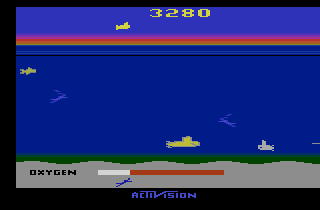
\includegraphics[width=.8\linewidth]{008182}
			\caption{}
			\label{seaquest:frame_1}
		\end{subfigure}%
		\begin{subfigure}{.5\textwidth}
			\centering
			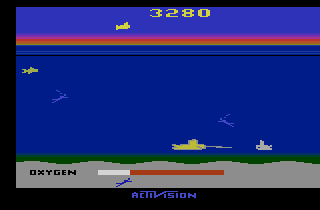
\includegraphics[width=.8\linewidth]{008185}
			\caption{}
			\label{seaquest:frame_2}
		\end{subfigure}\\[2ex]
		\begin{subfigure}{.5\textwidth}
			\centering
			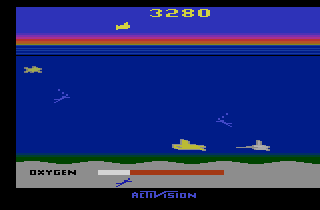
\includegraphics[width=.8\linewidth]{008188}
			\caption{}
			\label{seaquest:frame_3}
		\end{subfigure}%
		\begin{subfigure}{.5\textwidth}
			\centering
			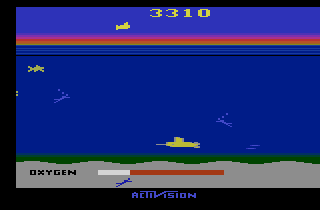
\includegraphics[width=.8\linewidth]{008191}
			\caption{}
			\label{seaquest:frame_4}
		\end{subfigure}%
		\caption[Hình ảnh một số ``frame'' của trò chơi \textit{Seaquest}]{Hình ảnh 4 ``frame'' của trò chơi \textit{Seaquest}.
		Ở ``frame'' đầu tiên (hình \ref{seaquest:frame_1}), tàu ngầm do hệ thống điều khiển ở giữa và tàu ngầm địch ở bên phải.
		Ở ``frame'' kế tiếp (hình \ref{seaquest:frame_2}), hệ thống thực hiện hành động phóng ngư lôi.
		Tiếp đó (hình \ref{seaquest:frame_3}), ngư lôi trúng tàu ngầm địch.
		Cuối cùng (hình \ref{seaquest:frame_4}), tàu ngầm địch bị phá huỷ cho điểm thưởng.
		Các ``frame'' này ứng với các giá trị trong đồ thị ở hình \ref{fig_seaquest_frames}.}
		\label{seaquest:frames}
	\end{figure}
	
	\begin{figure}
		\centering
		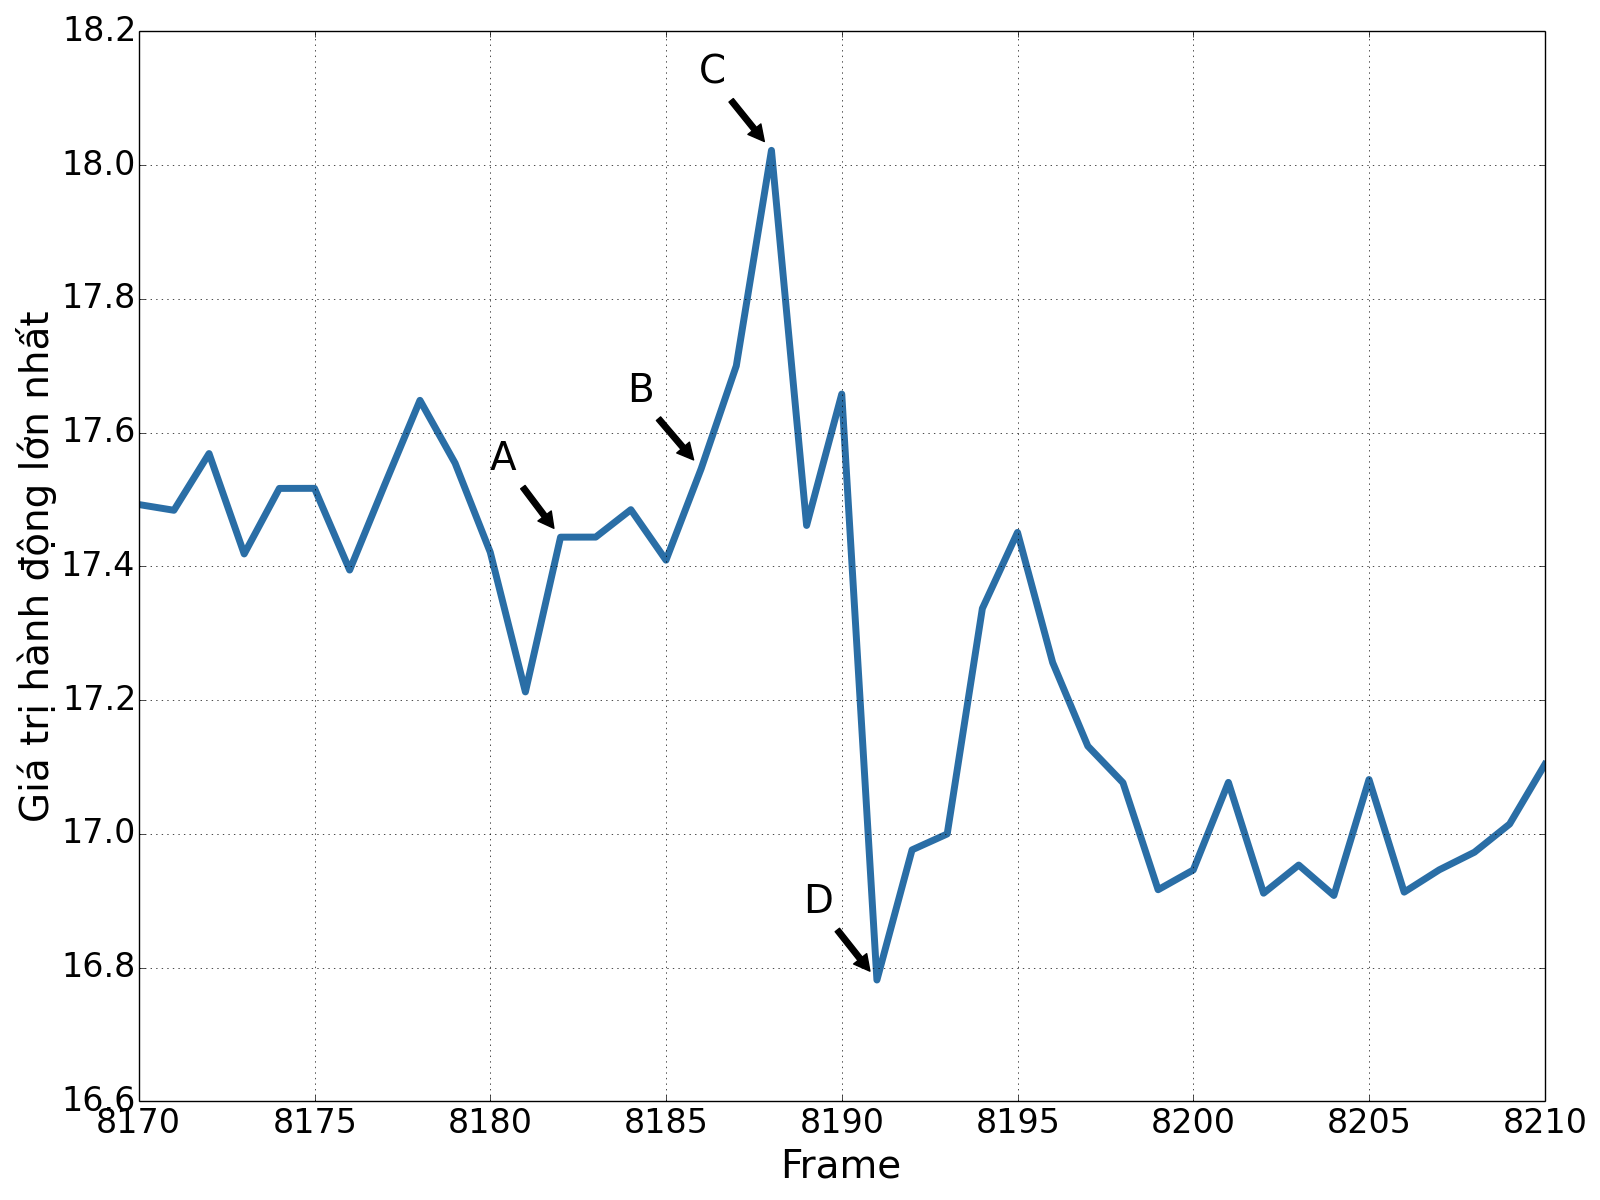
\includegraphics[width=\textwidth]{dqn_seaquest_frames}
		\caption[Đồ thị giá trị hành động của một số trạng thái trong một lần chơi game]{
		Đồ thị thể hiện giá trị hành động lớn nhất tại một số trạng thái; các trạng thái này ứng với các ``frame'' trò chơi \textit{Seaquest}.
		Tại ``frame'' được đánh dấu \textit{A}, giá trị hành động lớn nhất đang ở mức trung bình ứng với việc tàu ngầm của ta chưa thực hiện hành động gì ảnh hưởng đến điểm số.
		Tại ``frame'' \textit{B}, tàu ngầm của ta bắn ngư lôi về phía tàu ngầm địch.
		Mạng nơ-ron khi nhận được ``frame'' ảnh này ``hiểu'' được rằng nếu ngư lôi chạm vào địch thì ta sẽ nhận được điểm thưởng.
		Vì vậy, đồ thị giá trị bắt đầu tăng lên đến ''frame'' \textit{C}.
		Tại ``frame'' \textit{C}, ngư lôi trúng tàu ngầm địch nên việc nhận được điểm là chắc chắn; hàm giá trị biết được điều này nên đồ thị giá trị đạt đỉnh điểm tại đây.
		Sau khi nhận được điểm thưởng và tàu ngầm địch bị phá huỷ, mạng nơ-ron nhận thấy rằng xung quanh không có yếu tố nào có thể giúp tăng điểm số nên đánh giá ``frame'' \textit{D} có giá trị thấp.		
		}
		\label{fig_seaquest_frames}
	\end{figure}

	\chapter{Kết luận và hướng phát triển}


	
\renewcommand{\bibname}{
	\addcontentsline{toc}{chapter}{TÀI LIỆU THAM KHẢO}
	TÀI LIỆU THAM KHẢO
}
\bibliographystyle{Classes/IEEEtranS}
%\bibliographystyle{unsrt}
\bibliography{References/my_bib}
	
	
	%\input{Appendix}
	
\end{document}